\chapter{Building Abstractions with Data}
\label{Chapter 2}

\dictum[
	Hermann Weyl, \booktitle{The Mathematical Way of Thinking}
]{
	We now come to the decisive step of mathematical abstraction:
	we forget about what the symbols stand for.
	… [The mathematician] need not be idle;
	there are many operations which he may carry out with these symbols, without ever having to look at the things they stand for.
}

\vspace{2em}

\lettrine[findent=1pt]{W}{e concentrated in} \cref{Chapter 1} on computational processes and on the role of procedures in program design.
We saw how to use primitive data (numbers) and primitive operations (arithmetic operations), how to combine procedures to form compound procedures through composition, conditionals, and the use of parameters, and how to abstract procedures by using \code{define}.
We saw that a procedure can be regarded as a pattern for the local evolution of a process, and we classified, reasoned about, and performed simple algorithmic analyses of some common patterns for processes as embodied in procedures.
We also saw that higher-order procedures enhance the power of our language by enabling us to manipulate, and thereby to reason in terms of, general methods of computation.
This is much of the essence of programming.

In this chapter we are going to look at more complex data.
All the procedures in \cref{Chapter 1} operate on simple numerical data, and simple data are not sufficient for many of the problems we wish to address using computation.
Programs are typically designed to model complex phenomena, and more often than not one must construct computational objects that have several parts in order to model real-world phenomena that have several aspects.
Thus, whereas our focus in \cref{Chapter 1} was on building abstractions by combining procedures to form compound procedures, we turn in this chapter to another key aspect of any programming language:
the means it provides for building abstractions by combining data objects to form \newterm{compound data}.

Why do we want compound data in a programming language?
For the same reasons that we want compound procedures:
to elevate the conceptual level at which we can design our programs, to increase the modularity of our designs, and to enhance the expressive power of our language.
Just as the ability to define procedures enables us to deal with processes at a higher conceptual level than that of the primitive operations of the language, the ability to construct compound data objects enables us to deal with data at a higher conceptual level than that of the primitive data objects of the language.

Consider the task of designing a system to perform arithmetic with rational numbers.
We could imagine an operation \code{add-rat} that takes two rational numbers and produces their sum.
In terms of simple data, a rational number can be thought of as two integers:
a numerator and a denominator.
Thus, we could design a program in which each rational number would be represented by two integers (a numerator and a denominator) and where \code{add-rat} would be implemented by two procedures (one producing the numerator of the sum and one producing the denominator).
But this would be awkward, because we would then need to explicitly keep track of which numerators corresponded to which denominators.
In a system intended to perform many operations on many rational numbers, such bookkeeping details would clutter the programs substantially, to say nothing of what they would do to our minds.
It would be much better if we could “glue together” a numerator and denominator to form a pair---a \newterm{compound data object}---that our programs could manipulate in a way that would be consistent with regarding a rational number as a single conceptual unit.

The use of compound data also enables us to increase the modularity of our programs.
If we can manipulate rational numbers directly as objects in their own right, then we can separate the part of our program that deals with rational numbers per se from the details of how rational numbers may be represented as pairs of integers.
The general technique of isolating the parts of a program that deal with how data objects are represented from the parts of a program that deal with how data objects are used is a powerful design methodology called \newterm{data abstraction}.
We will see how data abstraction makes programs much easier to design, maintain, and modify.

The use of compound data leads to a real increase in the expressive power of our programming language.
Consider the idea of forming a “linear combination” \( ax + by \).
We might like to write a procedure that would accept \( a \), \( b \), \( x \), and \( y \) as arguments and return the value of \( ax + by \).
This presents no difficulty if the arguments are to be numbers, because we can readily define the procedure
\begin{scheme}
  (define (linear-combination a b x y)
    (+ (* a x) (* b y)))
\end{scheme}
But suppose we are not concerned only with numbers.
Suppose we would like to express, in procedural terms, the idea that one can form linear combinations whenever addition and multiplication are defined---for rational numbers, complex numbers, polynomials, or whatever.
We could express this as a procedure of the form
\begin{scheme}
  (define (linear-combination a b x y)
    (add (mul a x) (mul b y)))
\end{scheme}
where \code{add} and \code{mul} are not the primitive procedures \code{+} and \code{*} but rather more complex things that will perform the appropriate operations for whatever kinds of data we pass in as the arguments \code{a}, \code{b}, \code{x}, and \code{y}.
The key point is that the only thing \code{linear-combination} should need to know about \code{a}, \code{b}, \code{x}, and \code{y} is that the procedures \code{add} and \code{mul} will perform the appropriate manipulations.
From the perspective of the procedure \code{linear-combination}, it is irrelevant what \code{a}, \code{b}, \code{x}, and \code{y} are and even more irrelevant how they might happen to be represented in terms of more primitive data.
This same example shows why it is important that our programming language provide the ability to manipulate compound objects directly:
Without this, there is no way for a procedure such as \code{linear-combination} to pass its arguments along to \code{add} and \code{mul} without having to know their detailed structure.%
\footnote{
	The ability to directly manipulate procedures provides an analogous increase in the expressive power of a programming language.
	For example, in \cref{Section 1.3.1} we introduced the \code{sum} procedure, which takes a procedure \code{term} as an argument and computes the sum of the values of \code{term} over some specified interval.
	In order to define \code{sum}, it is crucial that we be able to speak of a procedure such as \code{term} as an entity in its own right, without regard for how \code{term} might be expressed with more primitive operations.
	Indeed, if we did not have the notion of “a procedure,” it is doubtful that we would ever even think of the possibility of defining an operation such as \code{sum}.
	Moreover, insofar as performing the summation is concerned, the details of how \code{term} may be constructed from more primitive operations are irrelevant.
}

We begin this chapter by implementing the rational-number arithmetic system mentioned above.
This will form the background for our discussion of compound data and data abstraction.
As with compound procedures, the main issue to be addressed is that of abstraction as a technique for coping with complexity, and we will see how data abstraction enables us to erect suitable \newterm{abstraction barriers} between different parts of a program.

We will see that the key to forming compound data is that a programming language should provide some kind of “glue” so that data objects can be combined to form more complex data objects.
There are many possible kinds of glue.
Indeed, we will discover how to form compound data using no special “data” operations at all, only procedures.
This will further blur the distinction between “procedure” and “data,” which was already becoming tenuous toward the end of \cref{Chapter 1}.
We will also explore some conventional techniques for representing sequences and trees.
One key idea in dealing with compound data is the notion of \newterm{closure}---that the glue we use for combining data objects should allow us to combine not only primitive data objects, but compound data objects as well.
Another key idea is that compound data objects can serve as \newterm{conventional interfaces} for combining program modules in mix-and-match ways.
We illustrate some of these ideas by presenting a simple graphics language that exploits closure.

We will then augment the representational power of our language by introducing \newterm{symbolic expressions}---data whose elementary parts can be arbitrary symbols rather than only numbers.
We explore various alternatives for representing sets of objects.
We will find that, just as a given numerical function can be computed by many different computational processes, there are many ways in which a given data structure can be represented in terms of simpler objects, and the choice of representation can have significant impact on the time and space requirements of processes that manipulate the data.
We will investigate these ideas in the context of symbolic differentiation, the representation of sets, and the encoding of information.

Next we will take up the problem of working with data that may be represented differently by different parts of a program.
This leads to the need to implement \newterm{generic operations}, which must handle many different types of data.
Maintaining modularity in the presence of generic operations requires more powerful abstraction barriers than can be erected with simple data abstraction alone.
In particular, we introduce \newterm{data-directed programming} as a technique that allows individual data representations to be designed in isolation and then combined \newterm{additively} (i.e., without modification).
To illustrate the power of this approach to system design, we close the chapter by applying what we have learned to the implementation of a package for performing symbolic arithmetic on polynomials, in which the coefficients of the polynomials can be integers, rational numbers, complex numbers, and even other polynomials.

\section{Introduction to Data Abstraction}
\label{Section 2.1}

In \link{Section 1.1.8}, we noted that a procedure used as an element in
creating a more complex procedure could be regarded not only as a collection of
particular operations but also as a procedural abstraction.  That is, the
details of how the procedure was implemented could be suppressed, and the
particular procedure itself could be replaced by any other procedure with the
same overall behavior.  In other words, we could make an abstraction that would
separate the way the procedure would be used from the details of how the
procedure would be implemented in terms of more primitive procedures.  The
analogous notion for compound data is called \newterm{data abstraction}.  Data
abstraction is a methodology that enables us to isolate how a compound data
object is used from the details of how it is constructed from more primitive
data objects.

The basic idea of data abstraction is to structure the programs that are to use
compound data objects so that they operate on ``abstract data.'' That is, our
programs should use data in such a way as to make no assumptions about the data
that are not strictly necessary for performing the task at hand.  At the same
time, a ``concrete'' data representation is defined independent of the programs
that use the data.  The interface between these two parts of our system will be
a set of procedures, called \newterm{selectors} and \newterm{constructors},
that implement the abstract data in terms of the concrete representation.  To
illustrate this technique, we will consider how to design a set of procedures
for manipulating rational numbers.



\subsection{Example: Arithmetic Operations\\ for Rational Numbers}
\label{Section 2.1.1}

Suppose we want to do arithmetic with rational numbers.  We want to be able to
add, subtract, multiply, and divide them and to test whether two rational
numbers are equal.

Let us begin by assuming that we already have a way of constructing a rational
number from a numerator and a denominator.  We also assume that, given a
rational number, we have a way of extracting (or selecting) its numerator and
its denominator.  Let us further assume that the constructor and selectors are
available as procedures:

\begin{itemize}

\item
\( \hbox{\tt(make-rat}\;\langle{n}\rangle\;\langle{d}\kern0.06em\rangle\hbox{\tt)} \) returns the rational number whose numerator is the integer \( \langle{n}\rangle \) and whose denominator is the integer
\( \langle{d}\kern0.06em\rangle \).

\item
\( \hbox{\tt(numer}\;\;\langle{x}\rangle\hbox{\tt)} \) returns the numerator of the rational number
\( \langle{x}\rangle \).

\item
\( \hbox{\tt(denom}\;\;\langle{x}\rangle\hbox{\tt)} \) returns the denominator of the rational number
\( \langle{x}\rangle \).

\end{itemize}

\noindent
We are using here a powerful strategy of synthesis: \newterm{wishful thinking}.
We haven't yet said how a rational number is represented, or how the procedures
\code{numer}, \code{denom}, and \code{make\-/rat} should be implemented.  Even
so, if we did have these three procedures, we could then add, subtract,
multiply, divide, and test equality by using the following relations:
\begin{comment}

\begin{example}
n_1   n_2   n_1 d_2 + n_2 d_1
--- + --- = -----------------
d_1   d_2        d_1 d_2

n_1   n_2   n_1 d_2 - n_2 d_1
--- - --- = -----------------
d_1   d_2        d_1 d_2

n_1   n_2   n_1 n_2
--- * --- = -------
d_1   d_2   d_1 d_2

n_1 / d_1   n_1 d_2
--------- = -------
n_2 / d_2   d_1 n_2

n_1   n_2
--- = ---  if and only if n_1 d_2 = n_2 d_1
d_1   d_2
\end{example}
\end{comment}
\begin{align*}
  {n_1 \over d_1} + {n_2 \over d_2} 	&= {n_1 d_2 + n_2 d_1 \over d_1 d_2}, \\
  {n_1 \over d_1} - {n_2 \over d_2} 	&= {n_1 d_2 - n_2 d_1 \over d_1 d_2}, \\
  {n_1 \over d_1} \cdot {n_2 \over d_2}	&= {n_1 n_2 \over d_1 d_2}, \\
  {n_1 / d_1} \over {n_2 / d_2} 	&= {n_1 d_2 \over d_1 n_2}, \\
  {n_1 \over d_1} 			&= {n_2 \over d_2} \quad
						{\rm\ if\ and\ only\ if\quad}
						n_1 d_2 = n_2 d_1.
\end{align*}
\noindent
We can express these rules as procedures:

\begin{scheme}
(define (add-rat x y)
  (make-rat (+ (* (numer x) (denom y))
               (* (numer y) (denom x)))
            (* (denom x) (denom y))))
(define (sub-rat x y)
  (make-rat (- (* (numer x) (denom y))
               (* (numer y) (denom x)))
            (* (denom x) (denom y))))
(define (mul-rat x y)
  (make-rat (* (numer x) (numer y))
            (* (denom x) (denom y))))
(define (div-rat x y)
  (make-rat (* (numer x) (denom y))
            (* (denom x) (numer y))))

(define (equal-rat? x y)
  (= (* (numer x) (denom y))
     (* (numer y) (denom x))))
\end{scheme}

Now we have the operations on rational numbers defined in terms of the selector
and constructor procedures \code{numer}, \code{denom}, and \code{make\-/rat}.
But we haven't yet defined these.  What we need is some way to glue together a
numerator and a denominator to form a rational number.

\subsubsection*{Pairs}

To enable us to implement the concrete level of our data abstraction, our
language provides a compound structure called a \newterm{pair}, which can be
constructed with the primitive procedure \code{cons}.  This procedure takes two
arguments and returns a compound data object that contains the two arguments as
parts.  Given a pair, we can extract the parts using the primitive procedures
\code{car} and \code{cdr}.\footnote{The name \code{cons} stands for
``construct.''  The names \code{car} and \code{cdr} derive from the original
implementation of Lisp on the \acronym{IBM 704}.  That machine had an addressing scheme
that allowed one to reference the ``address'' and ``decrement'' parts of a
memory location.  \code{car} stands for ``Contents of Address part of
Register'' and \code{cdr} (pronounced ``could-er'') stands for ``Contents of
Decrement part of Register.''} Thus, we can use \code{cons}, \code{car}, and
\code{cdr} as follows:

\begin{scheme}
(define x (cons 1 2))
(car x)
~\textit{1}~
(cdr x)
~\textit{2}~
\end{scheme}

\noindent
Notice that a pair is a data object that can be given a name and manipulated,
just like a primitive data object.  Moreover, \code{cons} can be used to form
pairs whose elements are pairs, and so on:

\begin{scheme}
(define x (cons 1 2))
(define y (cons 3 4))
(define z (cons x y))
(car (car z))
~\textit{1}~
(car (cdr z))
~\textit{3}~
\end{scheme}

\noindent
In \link{Section 2.2} we will see how this ability to combine pairs means that
pairs can be used as general-purpose building blocks to create all sorts of
complex data structures.  The single compound-data primitive \newterm{pair},
implemented by the procedures \code{cons}, \code{car}, and \code{cdr}, is the
only glue we need.  Data objects constructed from pairs are called
\newterm{list-structured} data.

\enlargethispage{\baselineskip}

\subsubsection*{Representing rational numbers}

Pairs offer a natural way to complete the rational-number system.  Simply
represent a rational number as a pair of two integers: a numerator and a
denominator.  Then \code{make\-/rat}, \code{numer}, and \code{denom} are readily
implemented as follows:\footnote{Another way to define the selectors and
constructor is

\begin{smallscheme}
(define make-rat cons)
(define numer car)
(define denom cdr)
\end{smallscheme}

The first definition associates the name \code{make\-/rat} with the value of the
expression \code{cons}, which is the primitive procedure that constructs pairs.
Thus \code{make\-/rat} and \code{cons} are names for the same primitive
constructor.

Defining selectors and constructors in this way is efficient: Instead of
\code{make\-/rat} \emph{calling} \code{cons}, \code{make\-/rat} \emph{is}
\code{cons}, so there is only one procedure called, not two, when
\code{make\-/rat} is called.  On the other hand, doing this defeats debugging
aids that trace procedure calls or put breakpoints on procedure calls: You may
want to watch \code{make\-/rat} being called, but you certainly don't want to
watch every call to \code{cons}.

We have chosen not to use this style of definition in this book.}

\begin{scheme}
(define (make-rat n d) (cons n d))
(define (numer x) (car x))
(define (denom x) (cdr x))
\end{scheme}

\noindent
Also, in order to display the results of our computations, we can print
rational numbers by printing the numerator, a slash, and the
denominator:\footnote{\code{display} is the Scheme primitive for printing data.
The Scheme primitive \code{newline} starts a new line for printing.  Neither of
these procedures returns a useful value, so in the uses of \code{print\-/rat}
below, we show only what \code{print\-/rat} prints, not what the interpreter
prints as the value returned by \code{print\-/rat}.}

\begin{scheme}
(define (print-rat x)
  (newline)
  (display (numer x))
  (display "/")
  (display (denom x)))
\end{scheme}

\noindent
Now we can try our rational-number procedures:

\begin{scheme}
(define one-half (make-rat 1 2))
(print-rat one-half)
~\textit{1/2}~
(define one-third (make-rat 1 3))
(print-rat (add-rat one-half one-third))
~\textit{5/6}~
(print-rat (mul-rat one-half one-third))
~\textit{1/6}~
(print-rat (add-rat one-third one-third))
~\textit{6/9}~
\end{scheme}

\noindent
As the final example shows, our rational-number implementation does not reduce
rational numbers to lowest terms.  We can remedy this by changing
\code{make\-/rat}. If we have a \code{gcd} procedure like the one in
\link{Section 1.2.5} that produces the greatest common divisor of two integers, we can
use \code{gcd} to reduce the numerator and the denominator to lowest terms
before constructing the pair:

\begin{scheme}
(define (make-rat n d)
  (let ((g (gcd n d)))
    (cons (/ n g) (/ d g))))
\end{scheme}

\noindent
Now we have

\begin{scheme}
(print-rat (add-rat one-third one-third))
~\textit{2/3}~
\end{scheme}

\noindent
as desired.  This modification was accomplished by changing the constructor
\code{make\-/rat} without changing any of the procedures (such as \code{add\-/rat}
and \code{mul\-/rat}) that implement the actual operations.

\begin{quote}
\heading{\phantomsection\label{Exercise 2.1}Exercise 2.1:} Define a better version of
\code{make\-/rat} that handles both positive and negative arguments.
\code{make\-/rat} should normalize the sign so that if the rational number is
positive, both the numerator and denominator are positive, and if the rational
number is negative, only the numerator is negative.
\end{quote}

\subsection{Abstraction Barriers}
\label{Section 2.1.2}

Before continuing with more examples of compound data and data abstraction, let
us consider some of the issues raised by the rational-number example.  We
defined the rational-number operations in terms of a constructor
\code{make\-/rat} and selectors \code{numer} and \code{denom}.  In general, the
underlying idea of data abstraction is to identify for each type of data object
a basic set of operations in terms of which all manipulations of data objects
of that type will be expressed, and then to use only those operations in
manipulating the data.

\begin{figure}[tb]
\phantomsection\label{Figure 2.1}
\centering
\begin{comment}
\begin{quote}
\heading{Figure 2.1:} Data-abstraction barriers in the rational-number package.

\begin{example}
        +------------------------------------+
--------| Programs that use rational numbers |--------
        +------------------------------------+
          Rational numbers in problem domain
            +---------------------------+
------------|   add-rat  sub-rat  ...   |-------------
            +---------------------------+
   Rational numbers as numerators and denominators
              +------------------------+
--------------| make-rat  numer  denom |--------------
              +------------------------+
              Rational numbers as pairs
                  +----------------+
------------------| cons  car  cdr |------------------
                  +----------------+
            However pairs are implemented
\end{example}
\end{quote}
\end{comment}
\includesvg[width=91mm]{fig/chap2/Fig2.1c.svg}
\begin{quote}
\heading{Figure 2.1:} Data-abstraction barriers in the rational-number package.
\end{quote}
\end{figure}

We can envision the structure of the rational-number system as shown in
\link{Figure 2.1}.  The horizontal lines represent \newterm{abstraction
barriers} that isolate different ``levels'' of the system.  At each level, the
barrier separates the programs (above) that use the data abstraction from the
programs (below) that implement the data abstraction.  Programs that use
rational numbers manipulate them solely in terms of the procedures supplied
``for public use'' by the rational-number package: \code{add\-/rat},
\code{sub\-/rat}, \code{mul\-/rat}, \code{div\-/rat}, and \code{equal\-/rat?}. These,
in turn, are implemented solely in terms of the constructor and selectors
\code{make\-/rat}, \code{numer}, and \code{denom}, which themselves are
implemented in terms of pairs.  The details of how pairs are implemented are
irrelevant to the rest of the rational-number package so long as pairs can be
manipulated by the use of \code{cons}, \code{car}, and \code{cdr}.  In effect,
procedures at each level are the interfaces that define the abstraction
barriers and connect the different levels.

This simple idea has many advantages.  One advantage is that it makes programs
much easier to maintain and to modify.  Any complex data structure can be
represented in a variety of ways with the primitive data structures provided by
a programming language.  Of course, the choice of representation influences the
programs that operate on it; thus, if the representation were to be changed at
some later time, all such programs might have to be modified accordingly.  This
task could be time-consuming and expensive in the case of large programs unless
the dependence on the representation were to be confined by design to a very
few program modules.

For example, an alternate way to address the problem of reducing rational
numbers to lowest terms is to perform the reduction whenever we access the
parts of a rational number, rather than when we construct it.  This leads to
different constructor and selector procedures:

\begin{scheme}
(define (make-rat n d) (cons n d))
(define (numer x)
  (let ((g (gcd (car x) (cdr x))))
    (/ (car x) g)))
(define (denom x)
  (let ((g (gcd (car x) (cdr x))))
    (/ (cdr x) g)))
\end{scheme}

\noindent
The difference between this implementation and the previous one lies in when we
compute the \code{gcd}.  If in our typical use of rational numbers we access
the numerators and denominators of the same rational numbers many times, it
would be preferable to compute the \code{gcd} when the rational numbers are
constructed.  If not, we may be better off waiting until access time to compute
the \code{gcd}.  In any case, when we change from one representation to the
other, the procedures \code{add\-/rat}, \code{sub\-/rat}, and so on do not have to
be modified at all.

Constraining the dependence on the representation to a few interface procedures
helps us design programs as well as modify them, because it allows us to
maintain the flexibility to consider alternate implementations.  To continue
with our simple example, suppose we are designing a rational-number package and
we can't decide initially whether to perform the \code{gcd} at construction
time or at selection time.  The data-abstraction methodology gives us a way to
defer that decision without losing the ability to make progress on the rest of
the system.

\begin{quote}
\heading{\phantomsection\label{Exercise 2.2}Exercise 2.2:} Consider the problem of
representing line segments in a plane.  Each segment is represented as a pair
of points: a starting point and an ending point.  Define a constructor
\code{make\-/segment} and selectors \code{start\-/segment} and \code{end\-/segment}
that define the representation of segments in terms of points.  Furthermore, a
point can be represented as a pair of numbers: the \( x \) coordinate and the
\( y \) coordinate.  Accordingly, specify a constructor \code{make\-/point} and
selectors \code{x\-/point} and \code{y\-/point} that define this representation.
Finally, using your selectors and constructors, define a procedure
\code{midpoint\-/segment} that takes a line segment as argument and returns its
midpoint (the point whose coordinates are the average of the coordinates of the
endpoints).  To try your procedures, you'll need a way to print points:

\begin{scheme}
(define (print-point p)
  (newline)
  (display "(")
  (display (x-point p))
  (display ",")
  (display (y-point p))
  (display ")"))
\end{scheme}
\end{quote}

\begin{quote}
\heading{\phantomsection\label{Exercise 2.3}Exercise 2.3:} Implement a representation for
rectangles in a plane.  (Hint: You may want to make use of \link{Exercise 2.2}.)
In terms of your constructors and selectors, create procedures that compute the
perimeter and the area of a given rectangle.  Now implement a different
representation for rectangles.  Can you design your system with suitable
abstraction barriers, so that the same perimeter and area procedures will work
using either representation?
\end{quote}

\subsection{What Is Meant by Data?}
\label{Section 2.1.3}

We began the rational-number implementation in \link{Section 2.1.1} by
implementing the rational-number operations \code{add\-/rat}, \code{sub\-/rat}, and
so on in terms of three unspecified procedures: \code{make\-/rat}, \code{numer},
and \code{denom}.  At that point, we could think of the operations as being
defined in terms of data objects---numerators, denominators, and rational
numbers---whose behavior was specified by the latter three procedures.

But exactly what is meant by \newterm{data}?  It is not enough to say
``whatever is implemented by the given selectors and constructors.''  Clearly,
not every arbitrary set of three procedures can serve as an appropriate basis
for the rational-number implementation.  We need to guarantee that, if we
construct a rational number \code{x} from a pair of integers \code{n} and
\code{d}, then extracting the \code{numer} and the \code{denom} of \code{x} and
dividing them should yield the same result as dividing \code{n} by \code{d}.
In other words, \code{make\-/rat}, \code{numer}, and \code{denom} must satisfy
the condition that, for any integer \code{n} and any non-zero integer \code{d},
if \code{x} is \code{(make\-/rat n d)}, then
\begin{comment}

\begin{example}
(numer x)    n
--------- = ---
(denom x)    d
\end{example}

\end{comment}

$$ {\hbox{\tt(numer x)} \over \hbox{\tt(denom x)}} = {{\tt n} \over {\tt d}}\,.  $$

In fact, this is the only condition \code{make\-/rat}, \code{numer}, and
\code{denom} must fulfill in order to form a suitable basis for a
rational-number representation.  In general, we can think of data as defined by
some collection of selectors and constructors, together with specified
conditions that these procedures must fulfill in order to be a valid
representation.\footnote{Surprisingly, this idea is very difficult to formulate
rigorously. There are two approaches to giving such a formulation.  One,
pioneered by C. A. R. \link{Hoare (1972)}, is known as the method of \newterm{abstract
models}.  It formalizes the ``procedures plus conditions'' specification as
outlined in the rational-number example above.  Note that the condition on the
rational-number representation was stated in terms of facts about integers
(equality and division).  In general, abstract models define new kinds of data
objects in terms of previously defined types of data objects.  Assertions about
data objects can therefore be checked by reducing them to assertions about
previously defined data objects.  Another approach, introduced by Zilles at
\acronym{MIT}, by Goguen, Thatcher, Wagner, and Wright at \acronym{IBM}
(see \link{Thatcher et al. 1978}),
and by Guttag at Toronto (see \link{Guttag 1977}), is called
\newterm{algebraic specification}.  It regards the ``procedures'' as elements
of an abstract algebraic system whose behavior is specified by axioms that
correspond to our ``conditions,'' and uses the techniques of abstract algebra
to check assertions about data objects.  Both methods are surveyed in the paper
by \link{Liskov and Zilles (1975)}.}

This point of view can serve to define not only ``high-level'' data objects,
such as rational numbers, but lower-level objects as well.  Consider the notion
of a pair, which we used in order to define our rational numbers.  We never
actually said what a pair was, only that the language supplied procedures
\code{cons}, \code{car}, and \code{cdr} for operating on pairs.  But the only
thing we need to know about these three operations is that if we glue two
objects together using \code{cons} we can retrieve the objects using \code{car}
and \code{cdr}.  That is, the operations satisfy the condition that, for any
objects \code{x} and \code{y}, if \code{z} is \code{(cons x y)} then \code{(car
z)} is \code{x} and \code{(cdr z)} is \code{y}.  Indeed, we mentioned that
these three procedures are included as primitives in our language.  However,
any triple of procedures that satisfies the above condition can be used as the
basis for implementing pairs.  This point is illustrated strikingly by the fact
that we could implement \code{cons}, \code{car}, and \code{cdr} without using
any data structures at all but only using procedures.  Here are the
definitions:

\begin{scheme}
(define (cons x y)
  (define (dispatch m)
    (cond ((= m 0) x)
          ((= m 1) y)
          (else (error "Argument not 0 or 1: CONS" m))))
  dispatch)
(define (car z) (z 0))
(define (cdr z) (z 1))
\end{scheme}

\noindent
This use of procedures corresponds to nothing like our intuitive notion of what
data should be.  Nevertheless, all we need to do to show that this is a valid
way to represent pairs is to verify that these procedures satisfy the condition
given above.

The subtle point to notice is that the value returned by \code{(cons x y)} is a
procedure---namely the internally defined procedure \code{dispatch}, which
takes one argument and returns either \code{x} or \code{y} depending on whether
the argument is 0 or 1.  Correspondingly, \code{(car z)} is defined to apply
\code{z} to 0.  Hence, if \code{z} is the procedure formed by \code{(cons x
y)}, then \code{z} applied to 0 will yield \code{x}. Thus, we have shown that
\code{(car (cons x y))} yields \code{x}, as desired.  Similarly, \code{(cdr
(cons x y))} applies the procedure returned by \code{(cons x y)} to 1, which
returns \code{y}.  Therefore, this procedural implementation of pairs is a
valid implementation, and if we access pairs using only \code{cons},
\code{car}, and \code{cdr} we cannot distinguish this implementation from one
that uses ``real'' data structures.

The point of exhibiting the procedural representation of pairs is not that our
language works this way (Scheme, and Lisp systems in general, implement pairs
directly, for efficiency reasons) but that it could work this way.  The
procedural representation, although obscure, is a perfectly adequate way to
represent pairs, since it fulfills the only conditions that pairs need to
fulfill.  This example also demonstrates that the ability to manipulate
procedures as objects automatically provides the ability to represent compound
data.  This may seem a curiosity now, but procedural representations of data
will play a central role in our programming repertoire.  This style of
programming is often called \newterm{message passing}, and we will be using it
as a basic tool in \link{Chapter 3} when we address the issues of modeling and
simulation.

\begin{quote}
\heading{\phantomsection\label{Exercise 2.4}Exercise 2.4:} Here is an alternative procedural
representation of pairs.  For this representation, verify that \code{(car (cons
x y))} yields \code{x} for any objects \code{x} and \code{y}.

\begin{scheme}
(define (cons x y)
  (lambda (m) (m x y)))
(define (car z)
  (z (lambda (p q) p)))
\end{scheme}

What is the corresponding definition of \code{cdr}? (Hint: To verify that this
works, make use of the substitution model of \link{Section 1.1.5}.)
\end{quote}

\begin{quote}
\heading{\phantomsection\label{Exercise 2.5}Exercise 2.5:} Show that we can represent pairs of
nonnegative integers using only numbers and arithmetic operations if we
represent the pair \( a \) and \( b \) as the integer that is the product \( 2^a 3^b \).
Give the corresponding definitions of the procedures \code{cons},
\code{car}, and \code{cdr}.
\end{quote}

\begin{quote}
\heading{\phantomsection\label{Exercise 2.6}Exercise 2.6:} In case representing pairs as
procedures wasn't mind-boggling enough, consider that, in a language that can
manipulate procedures, we can get by without numbers (at least insofar as
nonnegative integers are concerned) by implementing 0 and the operation of
adding 1 as

\begin{scheme}
(define zero (lambda (f) (lambda (x) x)))
(define (add-1 n)
  (lambda (f) (lambda (x) (f ((n f) x)))))
\end{scheme}

This representation is known as \newterm{Church numerals}, after its inventor,
Alonzo Church, the logician who invented the λ-calculus.

Define \code{one} and \code{two} directly (not in terms of \code{zero} and
\code{add\-/1}).  (Hint: Use substitution to evaluate \code{(add\-/1 zero)}).  Give
a direct definition of the addition procedure \code{+} (not in terms of
repeated application of \code{add\-/1}).
\end{quote}

\subsection{Extended Exercise: Interval Arithmetic}
\label{Section 2.1.4}

Alyssa P. Hacker is designing a system to help people solve engineering
problems.  One feature she wants to provide in her system is the ability to
manipulate inexact quantities (such as measured parameters of physical devices)
with known precision, so that when computations are done with such approximate
quantities the results will be numbers of known precision.

Electrical engineers will be using Alyssa's system to compute electrical
quantities.  It is sometimes necessary for them to compute the value of a
parallel equivalent resistance \( R_p \) of two resistors \( R_1 \), \( R_2 \)
using the formula
\begin{comment}

\begin{example}
            1
R_p = -------------
      1/R_1 + 1/R_2
\end{example}

\end{comment}

$$ R_p = {1 \over 1 / R_1 + 1 / R_2}.  $$

Resistance values are usually known only up to some tolerance guaranteed by the
manufacturer of the resistor.  For example, if you buy a resistor labeled ``6.8
ohms with 10\% tolerance'' you can only be sure that the resistor has a
resistance between \( 6.8 - 0.68 = 6.12 \) and \( 6.8 + 0.68 = 7.48 \) ohms.  Thus, if you
have a 6.8-ohm 10\% resistor in parallel with a 4.7-ohm 5\% resistor, the
resistance of the combination can range from about 2.58 ohms (if the two
resistors are at the lower bounds) to about 2.97 ohms (if the two resistors are
at the upper bounds).

Alyssa's idea is to implement ``interval arithmetic'' as a set of arithmetic
operations for combining ``intervals'' (objects that represent the range of
possible values of an inexact quantity).  The result of adding, subtracting,
multiplying, or dividing two intervals is itself an interval, representing the
range of the result.

Alyssa postulates the existence of an abstract object called an ``interval''
that has two endpoints: a lower bound and an upper bound.  She also presumes
that, given the endpoints of an interval, she can construct the interval using
the data constructor \code{make\-/interval}.  Alyssa first writes a procedure for
adding two intervals.  She reasons that the minimum value the sum could be is
the sum of the two lower bounds and the maximum value it could be is the sum of
the two upper bounds:

\begin{scheme}
(define (add-interval x y)
  (make-interval (+ (lower-bound x) (lower-bound y))
                 (+ (upper-bound x) (upper-bound y))))
\end{scheme}

\noindent
Alyssa also works out the product of two intervals by finding the minimum and
the maximum of the products of the bounds and using them as the bounds of the
resulting interval.  (\code{min} and \code{max} are primitives that find the
minimum or maximum of any number of arguments.)

\begin{scheme}
(define (mul-interval x y)
  (let ((p1 (* (lower-bound x) (lower-bound y)))
        (p2 (* (lower-bound x) (upper-bound y)))
        (p3 (* (upper-bound x) (lower-bound y)))
        (p4 (* (upper-bound x) (upper-bound y))))
    (make-interval (min p1 p2 p3 p4)
                   (max p1 p2 p3 p4))))
\end{scheme}

\noindent
To divide two intervals, Alyssa multiplies the first by the reciprocal of the
second.  Note that the bounds of the reciprocal interval are the reciprocal of
the upper bound and the reciprocal of the lower bound, in that order.

\begin{scheme}
(define (div-interval x y)
  (mul-interval
   x
   (make-interval (/ 1.0 (upper-bound y))
                  (/ 1.0 (lower-bound y)))))
\end{scheme}

\begin{quote}
\heading{\phantomsection\label{Exercise 2.7}Exercise 2.7:} Alyssa's program is incomplete
because she has not specified the implementation of the interval abstraction.
Here is a definition of the interval constructor:

\begin{scheme}
(define (make-interval a b) (cons a b))
\end{scheme}

Define selectors \code{upper\-/bound} and \code{lower\-/bound} to complete the
implementation.
\end{quote}

\begin{quote}
\heading{\phantomsection\label{Exercise 2.8}Exercise 2.8:} Using reasoning analogous to
Alyssa's, describe how the difference of two intervals may be computed.  Define
a corresponding subtraction procedure, called \code{sub\-/interval}.
\end{quote}

\begin{quote}
\heading{\phantomsection\label{Exercise 2.9}Exercise 2.9:} The \newterm{width} of an interval
is half of the difference between its upper and lower bounds.  The width is a
measure of the uncertainty of the number specified by the interval.  For some
arithmetic operations the width of the result of combining two intervals is a
function only of the widths of the argument intervals, whereas for others the
width of the combination is not a function of the widths of the argument
intervals.  Show that the width of the sum (or difference) of two intervals is
a function only of the widths of the intervals being added (or subtracted).
Give examples to show that this is not true for multiplication or division.
\end{quote}

\begin{quote}
\heading{\phantomsection\label{Exercise 2.10}Exercise 2.10:} Ben Bitdiddle, an expert systems
programmer, looks over Alyssa's shoulder and comments that it is not clear what
it means to divide by an interval that spans zero.  Modify Alyssa's code to
check for this condition and to signal an error if it occurs.
\end{quote}

\begin{quote}
\heading{\phantomsection\label{Exercise 2.11}Exercise 2.11:} In passing, Ben also cryptically
comments: ``By testing the signs of the endpoints of the intervals, it is
possible to break \code{mul\-/interval} into nine cases, only one of which
requires more than two multiplications.''  Rewrite this procedure using Ben's
suggestion.

After debugging her program, Alyssa shows it to a potential user, who complains
that her program solves the wrong problem.  He wants a program that can deal
with numbers represented as a center value and an additive tolerance; for
example, he wants to work with intervals such as \( 3.5 \pm 0.15 \) rather than
[3.35, 3.65].  Alyssa returns to her desk and fixes this problem by supplying
an alternate constructor and alternate selectors:

\begin{scheme}
(define (make-center-width c w)
  (make-interval (- c w) (+ c w)))
(define (center i)
  (/ (+ (lower-bound i) (upper-bound i)) 2))
(define (width i)
  (/ (- (upper-bound i) (lower-bound i)) 2))
\end{scheme}

Unfortunately, most of Alyssa's users are engineers.  Real engineering
situations usually involve measurements with only a small uncertainty, measured
as the ratio of the width of the interval to the midpoint of the interval.
Engineers usually specify percentage tolerances on the parameters of devices,
as in the resistor specifications given earlier.
\end{quote}

\begin{quote}
\heading{\phantomsection\label{Exercise 2.12}Exercise 2.12:} Define a constructor
\code{make\-/center\-/percent} that takes a center and a percentage tolerance and
produces the desired interval.  You must also define a selector \code{percent}
that produces the percentage tolerance for a given interval.  The \code{center}
selector is the same as the one shown above.
\end{quote}

\begin{quote}
\heading{\phantomsection\label{Exercise 2.13}Exercise 2.13:} Show that under the assumption of
small percentage tolerances there is a simple formula for the approximate
percentage tolerance of the product of two intervals in terms of the tolerances
of the factors.  You may simplify the problem by assuming that all numbers are
positive.

After considerable work, Alyssa P. Hacker delivers her finished system.
Several years later, after she has forgotten all about it, she gets a frenzied
call from an irate user, Lem E. Tweakit.  It seems that Lem has noticed that
the formula for parallel resistors can be written in two algebraically
equivalent ways:
\begin{comment}

\begin{example}
 R_1 R_2
---------
R_1 + R_2
\end{example}

\end{comment}

$$ R_1 R_2 \over R_1 + R_2 $$

\noindent
and
\begin{comment}

\begin{example}
      1
-------------
1/R_1 + 1/R_2
\end{example}

\end{comment}

$$ {1 \over 1 / R_1 + 1 / R_2}. $$

He has written the following two programs, each of which computes the
parallel-resistors formula differently:

\begin{scheme}
(define (par1 r1 r2)
  (div-interval (mul-interval r1 r2)
                (add-interval r1 r2)))
\end{scheme}

\begin{scheme}
(define (par2 r1 r2)
  (let ((one (make-interval 1 1)))
    (div-interval
     one (add-interval (div-interval one r1)
                       (div-interval one r2)))))
\end{scheme}
\vspace{0.3em}

Lem complains that Alyssa's program gives different answers for the two ways of
computing. This is a serious complaint.
\end{quote}

\begin{quote}
\heading{\phantomsection\label{Exercise 2.14}Exercise 2.14:} Demonstrate that Lem is right.
Investigate the behavior of the system on a variety of arithmetic
expressions. Make some intervals \( A \) and \( B \), and use them in computing the
expressions \( A / A \) and \( A / B \).  You will get the most insight by
using intervals whose width is a small percentage of the center value. Examine
the results of the computation in center-percent form (see \link{Exercise 2.12}).
\end{quote}

\begin{quote}
\heading{\phantomsection\label{Exercise 2.15}Exercise 2.15:} Eva Lu Ator, another user, has
also noticed the different intervals computed by different but algebraically
equivalent expressions. She says that a formula to compute with intervals using
Alyssa's system will produce tighter error bounds if it can be written in such
a form that no variable that represents an uncertain number is repeated.  Thus,
she says, \code{par2} is a ``better'' program for parallel resistances than
\code{par1}.  Is she right?  Why?
\end{quote}

\begin{quote}
\heading{\phantomsection\label{Exercise 2.16}Exercise 2.16:} Explain, in general, why
equivalent algebraic expressions may lead to different answers.  Can you devise
an interval-arithmetic package that does not have this shortcoming, or is this
task impossible?  (Warning: This problem is very difficult.)
\end{quote}

\section{Hierarchical Data and the Closure Property}
\label{Section 2.2}

As we have seen, pairs provide a primitive “glue” that we can use to construct compound data objects.
\link{Figure 2.2} shows a standard way to visualize a pair---in this case, the pair formed by \code{(cons 1 2)}.
In this representation, which is called \newterm{box-and-pointer notation}, each object is shown as a \newterm{pointer} to a box.
The box for a primitive object contains a representation of the object.
For example, the box for a number contains a numeral.
The box for a pair is actually a double box, the left part containing (a pointer to) the \code{car} of the pair and the right part containing the \code{cdr}.

We have already seen that \code{cons} can be used to combine not only numbers but pairs as well.
(You made use of this fact, or should have, in doing \link{Exercise 2.2} and \link{Exercise 2.3}.)
As a consequence, pairs provide a universal building block from which we can construct all sorts of data structures.
\link{Figure 2.3} shows two ways to use pairs to combine the numbers \( 1 \), \( 2 \), \( 3 \), and \( 4 \).

\begin{figure}[tb]
	\centering
	\includesvg[width=34mm]{fig/chap2/Fig2.2c.svg}
	\caption{
		Box-and-pointer representation of \code{(cons 1 2)}.
	}
	\label{Figure 2.2}
\end{figure}

\begin{figure}[tb]
	\centering
	\includesvg[width=96mm]{fig/chap2/Fig2.3c.svg}
	\caption{
		Two ways to combine 1, 2, 3, and 4 using pairs.
	}
	\label{Figure 2.3}
\end{figure}

The ability to create pairs whose elements are pairs is the essence of list structure’s importance as a representational tool.
We refer to this ability as the \newterm{closure property} of \code{cons}.
In general, an operation for combining data objects satisfies the closure property if the results of combining things with that operation can themselves be combined using the same operation.%
\footnote{
	The use of the word “closure” here comes from abstract algebra, where a set of elements is said to be closed under an operation if applying the operation to elements in the set produces an element that is again an element of the set.
	The Lisp community also (unfortunately) uses the word “closure” to describe a totally unrelated concept:
	A closure is an implementation technique for representing procedures with free variables.
	We do not use the word “closure” in this second sense in this book.
}
Closure is the key to power in any means of combination because it permits us to create \newterm{hierarchical} structures---structures made up of parts, which themselves are made up of parts, and so on.

From the outset of \link{Chapter 1}, we’ve made essential use of closure in dealing with procedures, because all but the very simplest programs rely on the fact that the elements of a combination can themselves be combinations.
In this section, we take up the consequences of closure for compound data.
We describe some conventional techniques for using pairs to represent sequences and trees, and we exhibit a graphics language that illustrates closure in a vivid way.%
\footnote{
	The notion that a means of combination should satisfy closure is a straightforward idea.
	Unfortunately, the data combiners provided in many popular programming languages do not satisfy closure, or make closure cumbersome to exploit.
	In Fortran or Basic, one typically combines data elements by assembling them into arrays---but one cannot form arrays whose elements are themselves arrays.
	Pascal and C admit structures whose elements are structures.
	However, this requires that the programmer manipulate pointers explicitly, and adhere to the restriction that each field of a structure can contain only elements of a prespecified form.
	Unlike Lisp with its pairs, these languages have no built-in general-purpose glue that makes it easy to manipulate compound data in a uniform way.
	This limitation lies behind Alan Perlis’s comment in his foreword to this book:
	“In Pascal the plethora of declarable data structures induces a specialization within functions that inhibits and penalizes casual cooperation.
	It is better to have 100 functions operate on one data structure than to have 10 functions operate on 10 data structures.”
}



\subsection{Representing Sequences}
\label{Section 2.2.1}

One of the useful structures we can build with pairs is a \newterm{sequence}---an ordered collection of data objects.
There are, of course, many ways to represent sequences in terms of pairs.
One particularly straightforward representation is illustrated in \link{Figure 2.4}, where the sequence 1, 2, 3, 4 is represented as a chain of pairs.
The \code{car} of each pair is the corresponding item in the chain, and the \code{cdr} of the pair is the next pair in the chain.
The \code{cdr} of the final pair signals the end of the sequence by pointing to a distinguished value that is not a pair, represented in box-and-pointer diagrams as a diagonal line and in programs as the value of the variable \code{nil}.

\begin{figure}[tb]
	\centering
	\includesvg[width=76mm]{fig/chap2/Fig2.4c.svg}
	\caption{
		The sequence 1, 2, 3, 4 represented as a chain of pairs.
	}
	\label{Figure 2.4}
\end{figure}
The entire sequence is constructed by nested \code{cons} operations:
\begin{scheme}
  (cons 1
        (cons 2
              (cons 3
                    (cons 4 nil))))
\end{scheme}

Such a sequence of pairs, formed by nested \code{cons}es, is called a \newterm{list}, and Scheme provides a primitive called \code{list} to help in constructing lists.%
\footnote{
	In this book, we use \newterm{list} to mean a chain of pairs terminated by the end-of-list marker.
 In contrast, the term \newterm{list structure} refers to any data structure made out of pairs, not just to lists.
}
The above sequence could be produced by \code{(list 1 2 3 4)}.
In general,
\begin{scheme}
  (list ⟨~\var{a}\ind{1}~⟩ ⟨~\var{a}\ind{2}~⟩ … ⟨~\var{a}\ind{n}~⟩)
\end{scheme}
is equivalent to
\begin{scheme}
  (cons ⟨~\var{a}\ind{1}~⟩ (cons ⟨~\var{a}\ind{2}~⟩ (cons … (cons ⟨~\var{a}\ind{n}~⟩ nil) …)))
\end{scheme}
Lisp systems conventionally print lists by printing the sequence of elements, enclosed in parentheses.
Thus, the data object in \link{Figure 2.4} is printed as \code{(1 2 3 4)}:
\begin{scheme}
  (define one-through-four (list 1 2 3 4))

  one-through-four
  ~\outprint{(1 2 3 4)}~
\end{scheme}
Be careful not to confuse the expression \code{(list 1 2 3 4)} with the list \code{(1 2 3 4)}, which is the result obtained when the expression is evaluated.
Attempting to evaluate the expression \code{(1 2 3 4)} will signal an error when the interpreter tries to apply the procedure \code{1} to arguments \code{2}, \code{3}, and \code{4}.

We can think of \code{car} as selecting the first item in the list, and of \code{cdr} as selecting the sublist consisting of all but the first item.
Nested applications of \code{car} and \code{cdr} can be used to extract the second, third, and subsequent items in the list.%
\footnote{
	Since nested applications of \code{car} and \code{cdr} are cumbersome to write, Lisp dialects provide abbreviations for them---for instance,
	\begin{smallscheme}
	  (cadr ⟨~\var{arg}~⟩) = (car (cdr ⟨~\var{arg}~⟩))
	\end{smallscheme}
	The names of all such procedures start with \code{c} and end with \code{r}.
	Each \code{a} between them stands for a \code{car} operation and each \code{d} for a \code{cdr} operation, to be applied in the same order in which they appear in the name.
	The names \code{car} and \code{cdr} persist because simple combinations like \code{cadr} are pronounceable.
}
The constructor \code{cons} makes a list like the original one, but with an additional item at the beginning.
\begin{scheme}
  (car one-through-four)
  ~\outprint{1}~

  (cdr one-through-four)
  ~\outprint{(2 3 4)}~

  (car (cdr one-through-four))
  ~\outprint{2}~

  (cons 10 one-through-four)
  ~\outprint{(10 1 2 3 4)}~

  (cons 5 one-through-four)
  ~\outprint{(5 1 2 3 4)}~
\end{scheme}
The value of \code{nil}, used to terminate the chain of pairs, can be thought of as a sequence of no elements, the \newterm{empty list}.
The word \newterm{nil} is a contraction of the Latin word \emph{nihil}, which means “nothing.”%
\footnote{
	It’s remarkable how much energy in the standardization of Lisp dialects has been dissipated in arguments that are literally over nothing:
	Should \code{nil} be an ordinary name?
	Should the value of \code{nil} be a symbol?
	Should it be a list?
	Should it be a pair?
	In Scheme, \code{nil} is an ordinary name, which we use in this section as a variable whose value is the end-of-list marker (just as \code{true} is an ordinary variable that has a true value).
	Other dialects of Lisp, including Common Lisp, treat \code{nil} as a special symbol.
	The authors of this book, who have endured too many language standardization brawls, would like to avoid the entire issue.
	Once we have introduced quotation in \link{Section 2.3}, we will denote the empty list as \code{'()} and dispense with the variable \code{nil} entirely.
}



\subsubsection*{List operations}

The use of pairs to represent sequences of elements as lists is accompanied by conventional programming techniques for manipulating lists by successively “\code{cdr}ing down” the lists.
For example, the procedure \code{list-ref} takes as arguments a list and a number \( n \) and returns the \( n \)\nth{th} item of the list.
It is customary to number the elements of the list beginning with \( 0 \).
The method for computing \code{list-ref} is the following:
\begin{itemize}

	\item
		For \( n = 0 \), \code{list-ref} should return the \code{car} of the list.

	\item
		Otherwise, \code{list-ref} should return the \( (n - 1) \)\nth{th} item of the \code{cdr} of the list.

\end{itemize}
\begin{scheme}
  (define (list-ref items n)
    (if (= n 0)
        (car items)
        (list-ref (cdr items) (- n 1))))

  (define squares (list 1 4 9 16 25))

  (list-ref squares 3)
  ~\outprint{16}~
\end{scheme}

Often we \code{cdr} down the whole list.
To aid in this, Scheme includes a  primitive predicate \code{null?}, which tests whether its argument is the empty list.
The procedure \code{length}, which returns the number of items in a list, illustrates this typical pattern of use:
\begin{scheme}
  (define (length items)
    (if (null? items)
        0
        (+ 1 (length (cdr items)))))

  (define odds (list 1 3 5 7))

  (length odds)
  ~\outprint{4}~
\end{scheme}
The \code{length} procedure implements a simple recursive plan.
The reduction  step is:
\begin{itemize}

	\item
		The \code{length} of any list is 1 plus the \code{length} of the \code{cdr} of
	the list.

\end{itemize}
This is applied successively until we reach the base case:
\begin{itemize}

	\item
		The \code{length} of the empty list is 0.

\end{itemize}
We could also compute \code{length} in an iterative style:
\begin{scheme}
  (define (length items)
    (define (length-iter a count)
      (if (null? a)
          count
          (length-iter (cdr a) (+ 1 count))))
    (length-iter items 0))
\end{scheme}

Another conventional programming technique is to “\code{cons} up” an answer list while \code{cdr}ing down a list, as in the procedure \code{append}, which takes two lists as arguments and combines their elements to make a new list:
\begin{scheme}
  (append squares odds)
  ~\outprint{(1 4 9 16 25 1 3 5 7)}~

  (append odds squares)
  ~\outprint{(1 3 5 7 1 4 9 16 25)}~
\end{scheme}
\code{append} is also implemented using a recursive plan.
To \code{append} lists \code{list1} and \code{list2}, do the following:
\begin{itemize}

	\item
		If \code{list1} is the empty list, then the result is just \code{list2}.

	\item
	Otherwise, \code{append} the \code{cdr} of \code{list1} and \code{list2}, and \code{cons} the \code{car} of \code{list1} onto the result:

\end{itemize}
\begin{scheme}
  (define (append list1 list2)
    (if (null? list1)
        list2
        (cons (car list1) (append (cdr list1) list2))))
\end{scheme}



\begin{exercise}
	\label{Exercise 2.17}
	Define a procedure \code{last-pair} that returns the list that contains only the last element of a given (nonempty) list:
	\begin{scheme}
	  (last-pair (list 23 72 149 34))
	  ~\outprint{(34)}~
	\end{scheme}
\end{exercise}



\begin{exercise}
	\label{Exercise 2.18}
	Define a procedure \code{reverse} that takes a list as argument and returns a list of the same elements in reverse order:
	\begin{scheme}
	  (reverse (list 1 4 9 16 25))
	  ~\outprint{(25 16 9 4 1)}~
	\end{scheme}
\end{exercise}



\begin{exercise}
	\label{Exercise 2.19}
	Consider the change-counting program of \link{Section 1.2.2}.
	It would be nice to be able to easily change the currency used by the program, so that we could compute the number of ways to change a British pound, for example.
	As the program is written, the knowledge of the currency is distributed partly into the procedure \code{first-denomination} and partly into the procedure \code{count-change} (which knows that there are five kinds of U.S. coins).
	It would be nicer to be able to supply a list of coins to be used for making change.

	We want to rewrite the procedure \code{cc} so that its second argument is a list of the values of the coins to use rather than an integer specifying which coins to use.
	We could then have lists that defined each kind of currency:
	\begin{scheme}
	  (define us-coins (list 50 25 10 5 1))

	  (define uk-coins (list 100 50 20 10 5 2 1 0.5))
	\end{scheme}
	We could then call \code{cc} as follows:
	\begin{scheme}
	  (cc 100 us-coins)
	  ~\outprint{292}~
	\end{scheme}
	To do this will require changing the program \code{cc} somewhat.
	It will still have the same form, but it will access its second argument differently, as follows:
	\begin{scheme}
	  (define (cc amount coin-values)
	    (cond ((= amount 0) 1)
	          ((or (< amount 0) (no-more? coin-values)) 0)
	          (else
	           (+ (cc amount
	                  (except-first-denomination
	                   coin-values))
	              (cc (- amount
	                     (first-denomination
	                      coin-values))
	                  coin-values)))))
	\end{scheme}
	Define the procedures \code{first-denomination}, \code{except-first-denomination}, and \code{no-more?} in terms of primitive operations on list structures.
	Does the order of the list \code{coin-values} affect the answer produced by \code{cc}?
	Why or why not?
\end{exercise}



\begin{exercise}
	\label{Exercise 2.20}
	The procedures \code{+}, \code{*}, and \code{list} take arbitrary numbers of arguments.
	One way to define such procedures is to use \code{define} with \newterm{dotted-tail notation}.
	In a procedure definition, a parameter list that has a dot before the last parameter name indicates that, when the procedure is called, the initial parameters (if any) will have as values the initial arguments, as usual, but the final parameter’s value will be a \newterm{list} of any remaining arguments.
	For instance, given the definition
	\begin{scheme}
	  (define (f x y . z) ⟨~\var{body}~⟩)
	\end{scheme}
	the procedure \code{f} can be called with two or more arguments.
	If we evaluate
	\begin{scheme}
	  (f 1 2 3 4 5 6)
	\end{scheme}
	then in the body of \code{f}, \code{x} will be \( 1 \), \code{y} will be \( 2 \), and \code{z} will be the list \code{(3 4 5 6)}.
	Given the definition
	\begin{scheme}
	  (define (g . w) ⟨~\var{body}~⟩)
	\end{scheme}
	the procedure \code{g} can be called with zero or more arguments.
	If we evaluate
	\begin{scheme}
	  (g 1 2 3 4 5 6)
	\end{scheme}
	then in the body of \code{g}, \code{w} will be the list \code{(1 2 3 4 5 6)}.%
	\footnote{
		To define \code{f} and \code{g} using \code{lambda} we would write
		\begin{smallscheme}
		  (define f (lambda (x y . z) ⟨~\var{body}~⟩))

		  (define g (lambda w ⟨~\var{body}~⟩))
		\end{smallscheme}
	}

	Use this notation to write a procedure \code{same-parity} that takes one or more integers and returns a list of all the arguments that have the same even-odd parity as the first argument.
	For example,
	\begin{scheme}
	  (same-parity 1 2 3 4 5 6 7)
	  ~\outprint{(1 3 5 7)}~

	  (same-parity 2 3 4 5 6 7)
	  ~\outprint{(2 4 6)}~
	\end{scheme}
\end{exercise}



\subsubsection*{Mapping over lists}

One extremely useful operation is to apply some transformation to each element in a list and generate the list of results.
For instance, the following procedure scales each number in a list by a given factor:
\begin{scheme}
  (define (scale-list items factor)
    (if (null? items)
        nil
        (cons (* (car items) factor)
              (scale-list (cdr items)
                          factor))))

  (scale-list (list 1 2 3 4 5) 10)
  ~\outprint{(10 20 30 40 50)}~
\end{scheme}

We can abstract this general idea and capture it as a common pattern expressed as a higher-order procedure, just as in \link{Section 1.3}.
The higher-order procedure here is called \code{map}.
\code{map} takes as arguments a procedure of one argument and a list, and returns a list of the results produced by applying the procedure to each element in the list%
\footnote{
	\label{Footnote 12} Scheme standardly provides a \code{map} procedure that is more general than the one described here.
	This more general \code{map} takes a procedure of \( n \) arguments, together with \( n \) lists, and applies the procedure to all the first elements of the lists, all the second elements of the lists, and so on, returning a list of the results.
	For example:
\begin{smallscheme}
  (map + (list 1 2 3) (list 40 50 60) (list 700 800 900))
  ~\outprint{(741 852 963)}~

  (map (lambda (x y) (+ x (* 2 y)))
       (list 1 2 3)
       (list 4 5 6))
  ~\outprint{(9 12 15)}~
\end{smallscheme}
}
\begin{scheme}
  (define (map proc items)
    (if (null? items)
        nil
        (cons (proc (car items))
              (map proc (cdr items)))))
  (map abs (list -10 2.5 -11.6 17))
  ~\outprint{(10 2.5 11.6 17)}~

  (map (lambda (x) (* x x)) (list 1 2 3 4))
  ~\outprint{(1 4 9 16)}~
\end{scheme}
Now we can give a new definition of \code{scale-list} in terms of \code{map}:
\begin{scheme}
  (define (scale-list items factor)
    (map (lambda (x) (* x factor))
         items))
\end{scheme}
\code{map} is an important construct, not only because it captures a common pattern, but because it establishes a higher level of abstraction in dealing with lists.
In the original definition of \code{scale-list}, the recursive structure of the program draws attention to the element-by-element processing of the list.
Defining \code{scale-list} in terms of \code{map} suppresses that level of detail and emphasizes that scaling transforms a list of elements to a list of results.
The difference between the two definitions is not that the computer is performing a different process (it isn’t) but that we think about the process differently.
In effect, \code{map} helps establish an abstraction barrier that isolates the implementation of procedures that transform lists from the details of how the elements of the list are extracted and combined.
Like the barriers shown in \link{Figure 2.1}, this abstraction gives us the flexibility to change the low-level details of how sequences are implemented, while preserving the conceptual framework of operations that transform sequences to sequences.
\link{Section 2.2.3} expands on this use of sequences as a framework for organizing programs.



\begin{exercise}
	\label{Exercise 2.21}
	The procedure \code{square-list} takes a list of numbers as argument and returns a list of the squares of those numbers.
	\begin{scheme}
	  (square-list (list 1 2 3 4))
	  ~\outprint{(1 4 9 16)}~
	\end{scheme}
	Here are two different definitions of \code{square-list}.
	Complete both of them by filling in the missing expressions:
	\begin{scheme}
	  (define (square-list items)
	    (if (null? items)
	        nil
	        (cons ⟨??⟩ ⟨??⟩)))

	  (define (square-list items)
	    (map ⟨??⟩ ⟨??⟩))
	\end{scheme}
\end{exercise}



\begin{exercise}
	\label{Exercise 2.22}
	Louis Reasoner tries to rewrite the first \code{square-list} procedure of \link{Exercise 2.21} so that it evolves an iterative process:
	\begin{scheme}
	  (define (square-list items)
	    (define (iter things answer)
	      (if (null? things)
	          answer
	          (iter (cdr things)
	                (cons (square (car things))
	                      answer))))
	    (iter items nil))
	\end{scheme}
	Unfortunately, defining \code{square-list} this way produces the answer list in the reverse order of the one desired.
	Why?

	Louis then tries to fix his bug by interchanging the arguments to \code{cons}:
	\begin{scheme}
	  (define (square-list items)
	    (define (iter things answer)
	      (if (null? things)
	          answer
	          (iter (cdr things)
	                (cons answer
	                      (square (car things))))))
	    (iter items nil))
	\end{scheme}
	This doesn’t work either.
	Explain.
\end{exercise}



\begin{exercise}
	\label{Exercise 2.23}
	The procedure \code{for-each} is similar to \code{map}.
	It takes as arguments a procedure and a list of elements.
	However, rather than forming a list of the results, \code{for-each} just applies the procedure to each of the elements in turn, from left to right.
	The values returned by applying the procedure to the elements are not used at all---\code{for-each} is used with procedures that perform an action, such as printing.
	For example,
	\begin{scheme}
	  (for-each (lambda (x)
	              (newline)
	              (display x))
	            (list 57 321 88))
	  ~\outprint{57}~
	  ~\outprint{321}~
	  ~\outprint{88}~
	\end{scheme}
	The value returned by the call to \code{for-each} (not illustrated above) can be something arbitrary, such as true.
	Give an implementation of \code{for-each}.
\end{exercise}



\subsection{Hierarchical Structures}
\label{Section 2.2.2}

The representation of sequences in terms of lists generalizes naturally to represent sequences whose elements may themselves be sequences.
For example, we can regard the object \code{((1 2) 3 4)} constructed by
\begin{scheme}
  (cons (list 1 2) (list 3 4))
\end{scheme}
as a list of three items, the first of which is itself a list, \code{(1 2)}.
Indeed, this is suggested by the form in which the result is printed by the interpreter.
\link{Figure 2.5} shows the representation of this structure in terms of pairs.

\begin{figure}[tb]
	\centering
	\includesvg[width=91mm]{fig/chap2/Fig2.5c.svg}
	\caption{
		Structure formed by \code{(cons (list 1 2) (list 3 4))}.
	}
	\label{Figure 2.5}
\end{figure}

Another way to think of sequences whose elements are sequences is as \newterm{trees}.
The elements of the sequence are the branches of the tree, and elements that are themselves sequences are subtrees.
\link{Figure 2.6} shows the structure in \link{Figure 2.5} viewed as a tree.


\begin{figure}[tb]
	\label{Figure 2.6}
	\centering
	\includesvg[width=22mm]{fig/chap2/Fig2.6a.svg}
	\caption{
		The list structure in \link{Figure 2.5} viewed as a tree.
	}
\end{figure}
Recursion is a natural tool for dealing with tree structures, since we can often reduce operations on trees to operations on their branches, which reduce in turn to operations on the branches of the branches, and so on, until we reach the leaves of the tree.
As an example, compare the \code{length} procedure of \link{Section 2.2.1} with the \code{count-leaves} procedure, which returns the total number of leaves of a tree:
\begin{scheme}
  (define x (cons (list 1 2) (list 3 4)))

  (length x)
  ~\outprint{3}~

  (count-leaves x)
  ~\outprint{4}~

  (list x x)
  ~\outprint{(((1 2) 3 4) ((1 2) 3 4))}~

  (length (list x x))
  ~\outprint{2}~

  (count-leaves (list x x))
  ~\outprint{8}~
\end{scheme}

To implement \code{count-leaves}, recall the recursive plan for computing
\code{length}:
\begin{itemize}

	\item
		\code{length} of a list \code{x} is 1 plus \code{length} of the \code{cdr} of \code{x}.

	\item
		\code{length} of the empty list is 0.

\end{itemize}
\code{count-leaves} is similar.  The value for the empty list is the same:
\begin{itemize}

	\item
		\code{count-leaves} of the empty list is 0.

\end{itemize}
But in the reduction step, where we strip off the \code{car} of the list, we must take into account that the \code{car} may itself be a tree whose leaves we need to count.
Thus, the appropriate reduction step is
\begin{itemize}

	\item
		\code{count-leaves} of a tree \code{x} is \code{count-leaves} of the \code{car}  of \code{x} plus \code{count-leaves} of the \code{cdr} of \code{x}.

\end{itemize}
Finally, by taking \code{car}s we reach actual leaves, so we need another base
case:
\begin{itemize}

	\item
		\code{count-leaves} of a leaf is 1.

\end{itemize}
To aid in writing recursive procedures on trees, Scheme provides the primitive predicate \code{pair?}, which tests whether its argument is a pair.
Here is the complete procedure:%
\footnote{
	The order of the first two clauses in the \code{cond} matters, since the empty list satisfies \code{null?} and also is not a pair.
}
\begin{scheme}
  (define (count-leaves x)
    (cond ((null? x) 0)
          ((not (pair? x)) 1)
          (else (+ (count-leaves (car x))
                   (count-leaves (cdr x))))))
\end{scheme}



\begin{exercise}
	\label{Exercise 2.24}
	Suppose we evaluate the expression \code{(list 1 (list 2 (list 3 4)))}.
	Give the result printed by the interpreter, the corresponding box-and-pointer structure, and the interpretation of this as a tree (as in \link{Figure 2.6}).
\end{exercise}



\begin{exercise}
	\label{Exercise 2.25}
	Give combinations of \code{car}s and \code{cdr}s that will pick 7 from each of the following lists:
	\begin{scheme}
	  (1 3 (5 7) 9)

	  ((7))

	  (1 (2 (3 (4 (5 (6 7))))))
	\end{scheme}
\end{exercise}



\begin{exercise}
	\label{Exercise 2.26}
	Suppose we define \code{x} and \code{y} to be two lists:
	\begin{scheme}
	  (define x (list 1 2 3))

	  (define y (list 4 5 6))
	\end{scheme}
	What result is printed by the interpreter in response to evaluating each of the
	following expressions:
	\begin{scheme}
	  (append x y)

	  (cons x y)

	  (list x y)
	\end{scheme}
\end{exercise}



\begin{exercise}
	\label{Exercise 2.27}
	Modify your \code{reverse} procedure of \link{Exercise 2.18} to produce a \code{deep-reverse} procedure that takes a list as argument and returns as its value the list with its elements reversed and with all sublists deep-reversed as well.
	For example,
	\begin{scheme}
	  (define x (list (list 1 2) (list 3 4)))

	  x
	  ~\outprint{((1 2) (3 4))}~

	  (reverse x)
	  ~\outprint{((3 4) (1 2))}~

	  (deep-reverse x)
	  ~\outprint{((4 3) (2 1))}~
	\end{scheme}
\end{exercise}



\begin{exercise}
	\label{Exercise 2.28}
	Write a procedure \code{fringe} that takes as argument a tree (represented as a list) and returns a list whose elements are all the leaves of the tree arranged in left-to-right order.
	For example,
	\begin{scheme}
	  (define x (list (list 1 2) (list 3 4)))

	  (fringe x)
	  ~\outprint{(1 2 3 4)}~

	  (fringe (list x x))
	  ~\outprint{(1 2 3 4 1 2 3 4)}~
	\end{scheme}
\end{exercise}



\begin{exercise}
	\label{Exercise 2.29}
	A binary mobile consists of two branches, a left branch and a right branch.
	Each branch is a rod of a certain length, from which hangs either a weight or another binary mobile.
	We can represent a binary mobile using compound data by constructing it from two branches (for example, using \code{list}):
	\begin{scheme}
	  (define (make-mobile left right)
	    (list left right))
	\end{scheme}
	A branch is constructed from a \code{length} (which must be a number) together with a \code{structure}, which may be either a number (representing a simple weight) or another mobile:
	\begin{scheme}
	  (define (make-branch length structure)
	    (list length structure))
	\end{scheme}
	\begin{enumerate}[label = \alph*., leftmargin = *]

		\item
			Write the corresponding selectors \code{left-branch} and \code{right-branch}, which return the branches of a mobile, and \code{branch-length} and \code{branch-structure}, which return the components of a branch.

		\item
			Using your selectors, define a procedure \code{total-weight} that returns the total weight of a mobile.

		\item
			A mobile is said to be \newterm{balanced} if the torque applied by its top-left branch is equal to that applied by its top-right branch (that is, if the length of the left rod multiplied by the weight hanging from that rod is equal to the corresponding product for the right side) and if each of the submobiles hanging off its branches is balanced.
			Design a predicate that tests whether a binary mobile is balanced.

		\item
			Suppose we change the representation of mobiles so that the constructors are
			\begin{scheme}
			  (define (make-mobile left right) (cons left right))

			  (define (make-branch length structure)
			    (cons length structure))
			\end{scheme}
			How much do you need to change your programs to convert to the new representation?

	\end{enumerate}
\end{exercise}



\subsubsection*{Mapping over trees}

Just as \code{map} is a powerful abstraction for dealing with sequences, \code{map} together with recursion is a powerful abstraction for dealing with trees.
For instance, the \code{scale-tree} procedure, analogous to \code{scale-list} of \link{Section 2.2.1}, takes as arguments a numeric factor and a tree whose leaves are numbers.
It returns a tree of the same shape, where each number is multiplied by the factor.
The recursive plan for \code{scale-tree} is similar to the one for \code{count-leaves}:
\begin{scheme}
  (define (scale-tree tree factor)
    (cond ((null? tree) nil)
          ((not (pair? tree)) (* tree factor))
          (else (cons (scale-tree (car tree) factor)
                      (scale-tree (cdr tree) factor)))))

  (scale-tree (list 1 (list 2 (list 3 4) 5) (list 6 7)) 10)
  ~\outprint{(10 (20 (30 40) 50) (60 70))}~
\end{scheme}

Another way to implement \code{scale-tree} is to regard the tree as a sequence of sub-trees and use \code{map}.
We map over the sequence, scaling each sub-tree in turn, and return the list of results.
In the base case, where the tree is a leaf, we simply multiply by the factor:
\begin{scheme}
  (define (scale-tree tree factor)
    (map (lambda (sub-tree)
           (if (pair? sub-tree)
               (scale-tree sub-tree factor)
               (* sub-tree factor)))
         tree))
\end{scheme}
Many tree operations can be implemented by similar combinations of sequence
operations and recursion.



\begin{exercise}
	\label{Exercise 2.30}
	Define a procedure \code{square-tree} analogous to the \code{square-list} procedure of \link{Exercise 2.21}.
	That is, \code{square-tree} should behave as follows:
	\begin{scheme}
	  (square-tree
	   (list 1
	         (list 2 (list 3 4) 5)
	         (list 6 7)))
	  ~\outprint{(1 (4 (9 16) 25) (36 49))}~
	\end{scheme}
	Define \code{square-tree} both directly (i.e., without using any higher-order procedures) and also by using \code{map} and recursion.
\end{exercise}



\begin{exercise}
	\label{Exercise 2.31}
	Abstract your answer to \link{Exercise 2.30} to produce a procedure \code{tree-map} with the property that \code{square-tree} could be defined as
	\begin{scheme}
	  (define (square-tree tree) (tree-map square tree))
	\end{scheme}
\end{exercise}



\begin{exercise}
	\label{Exercise 2.32}
	We can represent a set as a list of distinct elements, and we can represent the set of all subsets of the set as a list of lists.
	For example, if the set is \code{(1 2 3)}, then the set of all subsets is \code{(() (3) (2) (2 3) (1) (1 3) (1 2) (1 2 3))}.
	Complete the following definition of a procedure that generates the set of subsets of a set and give a clear explanation of why it works:
	\begin{scheme}
	  (define (subsets s)
	    (if (null? s)
	        (list nil)
	        (let ((rest (subsets (cdr s))))
	          (append rest (map ⟨??⟩ rest)))))
	\end{scheme}
\end{exercise}



\subsection{Sequences as Conventional Interfaces}
\label{Section 2.2.3}

In working with compound data, we’ve stressed how data abstraction permits us to design programs without becoming enmeshed in the details of data representations, and how abstraction preserves for us the flexibility to experiment with alternative representations.
In this section, we introduce another powerful design principle for working with data structures---the use of \newterm{conventional interfaces}.

In \link{Section 1.3} we saw how program abstractions, implemented as higher-order procedures, can capture common patterns in programs that deal with numerical data.
Our ability to formulate analogous operations for working with compound data depends crucially on the style in which we manipulate our data structures.
Consider, for example, the following procedure, analogous to the \code{count-leaves} procedure of \link{Section 2.2.2}, which takes a tree as argument and computes the sum of the squares of the leaves that are odd:
\begin{scheme}
  (define (sum-odd-squares tree)
    (cond ((null? tree) 0)
          ((not (pair? tree))
           (if (odd? tree) (square tree) 0))
          (else (+ (sum-odd-squares (car tree))
                   (sum-odd-squares (cdr tree))))))
\end{scheme}
On the surface, this procedure is very different from the following one, which constructs a list of all the even Fibonacci numbers \( \Fib(k) \), where \( k \) is less than or equal to a given integer \( n \):
\begin{scheme}
  (define (even-fibs n)
    (define (next k)
      (if (> k n)
          nil
          (let ((f (fib k)))
            (if (even? f)
                (cons f (next (+ k 1)))
                (next (+ k 1))))))
    (next 0))
\end{scheme}

Despite the fact that these two procedures are structurally very different, a more abstract description of the two computations reveals a great deal of similarity.
The first program
\begin{itemize}

	\item
		enumerates the leaves of a tree;

	\item
		filters them, selecting the odd ones;

	\item
		squares each of the selected ones; and

	\item
		accumulates the results using \code{+}, starting with \( 0 \).

\end{itemize}
The second program
\begin{itemize}

	\item
		enumerates the integers from \( 0 \) to \( n \);

	\item
		computes the Fibonacci number for each integer;

	\item
		filters them, selecting the even ones; and

	\item
		accumulates the results using \code{cons}, starting with the empty list.

\end{itemize}

A signal-processing engineer would find it natural to conceptualize these processes in terms of signals flowing through a cascade of stages, each of which implements part of the program plan, as shown in \link{Figure 2.7}.
In \code{sum-odd-squares}, we begin with an \newterm{enumerator}, which generates a “signal” consisting of the leaves of a given tree.
This signal is passed through a \newterm{filter}, which eliminates all but the odd elements.
The resulting signal is in turn passed through a \newterm{map}, which is a “transducer” that applies the \code{square} procedure to each element.
The output of the map is then fed to an \newterm{accumulator}, which combines the elements using \code{+}, starting from an initial \( 0 \).
The plan for \code{even-fibs} is analogous.

\begin{figure}[tb]
	\centering
	\includesvg[width=111mm]{fig/chap2/Fig2.7d.svg}
	\caption{
		The signal-flow plans for the procedures \code{sum-odd-squares} (top) and \code{even-fibs} (bottom) reveal the commonality between the two programs.
	}
	\label{Figure 2.7}
\end{figure}

Unfortunately, the two procedure definitions above fail to exhibit this signal-flow structure.
For instance, if we examine the \code{sum-odd-squares} procedure, we find that the enumeration is implemented partly by the \code{null?} and \code{pair?} tests and partly by the tree-recursive structure of the procedure.
Similarly, the accumulation is found partly in the tests and partly in the addition used in the recursion.
In general, there are no distinct parts of either procedure that correspond to the elements in the signal-flow description.
Our two procedures decompose the computations in a different way, spreading the enumeration over the program and mingling it with the map, the filter, and the accumulation.
If we could organize our programs to make the signal-flow structure manifest in the procedures we write, this would increase the conceptual clarity of the resulting code.



\subsubsection*{Sequence Operations}

The key to organizing programs so as to more clearly reflect the signal-flow structure is to concentrate on the “signals” that flow from one stage in the process to the next.
If we represent these signals as lists, then we can use list operations to implement the processing at each of the stages.
For instance, we can implement the mapping stages of the signal-flow diagrams using the \code{map} procedure from \link{Section 2.2.1}:
\begin{scheme}
  (map square (list 1 2 3 4 5))
  ~\outprint{(1 4 9 16 25)}~
\end{scheme}

Filtering a sequence to select only those elements that satisfy a given predicate is accomplished by
\begin{scheme}
  (define (filter predicate sequence)
    (cond ((null? sequence) nil)
          ((predicate (car sequence))
           (cons (car sequence)
                 (filter predicate (cdr sequence))))
          (else (filter predicate (cdr sequence)))))
\end{scheme}
For example,
\begin{scheme}
  (filter odd? (list 1 2 3 4 5))
  ~\outprint{(1 3 5)}~
\end{scheme}

Accumulations can be implemented by
\begin{scheme}
  (define (accumulate op initial sequence)
    (if (null? sequence)
        initial
        (op (car sequence)
            (accumulate op initial (cdr sequence)))))

  (accumulate + 0 (list 1 2 3 4 5))
  ~\outprint{15}~

  (accumulate * 1 (list 1 2 3 4 5))
  ~\outprint{120}~

  (accumulate cons nil (list 1 2 3 4 5))
  ~\outprint{(1 2 3 4 5)}~
\end{scheme}

All that remains to implement signal-flow diagrams is to enumerate the sequence of elements to be processed.
For \code{even-fibs}, we need to generate the sequence of integers in a given range, which we can do as follows:
\begin{scheme}
  (define (enumerate-interval low high)
    (if (> low high)
        nil
        (cons low (enumerate-interval (+ low 1) high))))

  (enumerate-interval 2 7)
  ~\outprint{(2 3 4 5 6 7)}~
\end{scheme}
To enumerate the leaves of a tree, we can use%
\footnote{
	This is, in fact, precisely the \code{fringe} procedure from \link{Exercise 2.28}.
	Here we’ve renamed it to emphasize that it is part of a family of general sequence-manipulation procedures.
}
\begin{scheme}
  (define (enumerate-tree tree)
    (cond ((null? tree) nil)
          ((not (pair? tree)) (list tree))
          (else (append (enumerate-tree (car tree))
                        (enumerate-tree (cdr tree))))))

  (enumerate-tree (list 1 (list 2 (list 3 4)) 5))
  ~\outprint{(1 2 3 4 5)}~
\end{scheme}

Now we can reformulate \code{sum-odd-squares} and \code{even-fibs} as in the signal-flow diagrams.
For \code{sum-odd-squares}, we enumerate the sequence of leaves of the tree, filter this to keep only the odd numbers in the sequence, square each element, and sum the results:
\begin{scheme}
  (define (sum-odd-squares tree)
    (accumulate
     + 0 (map square (filter odd? (enumerate-tree tree)))))
\end{scheme}
For \code{even-fibs}, we enumerate the integers from \( 0 \) to \( n \), generate the Fibonacci number for each of these integers, filter the resulting sequence to keep only the even elements, and accumulate the results into a list:
\begin{scheme}
  (define (even-fibs n)
    (accumulate
     cons
     nil
     (filter even? (map fib (enumerate-interval 0 n)))))
\end{scheme}

The value of expressing programs as sequence operations is that this helps us make program designs that are modular, that is, designs that are constructed by combining relatively independent pieces.
We can encourage modular design by providing a library of standard components together with a conventional interface for connecting the components in flexible ways.

Modular construction is a powerful strategy for controlling complexity in engineering design.
In real signal-processing applications, for example, designers regularly build systems by cascading elements selected from standardized families of filters and transducers.
Similarly, sequence operations provide a library of standard program elements that we can mix and match.
For instance, we can reuse pieces from the \code{sum-odd-squares} and \code{even-fibs} procedures in a program that constructs a list of the squares of the first \( n + 1 \) Fibonacci numbers:
\begin{scheme}
  (define (list-fib-squares n)
    (accumulate
     cons
     nil
     (map square (map fib (enumerate-interval 0 n)))))

  (list-fib-squares 10)
  ~\outprint{(0 1 1 4 9 25 64 169 441 1156 3025)}~
\end{scheme}
We can rearrange the pieces and use them in computing the product of the squares of the odd
integers in a sequence:
\begin{scheme}
  (define (product-of-squares-of-odd-elements sequence)
    (accumulate * 1 (map square (filter odd? sequence))))

  (product-of-squares-of-odd-elements (list 1 2 3 4 5))
  ~\outprint{225}~
\end{scheme}

We can also formulate conventional data-processing applications in terms of sequence operations.
Suppose we have a sequence of personnel records and we want to find the salary of the highest-paid programmer.
Assume that we have a selector \code{salary} that returns the salary of a record, and a predicate \code{programmer?} that tests if a record is for a programmer.
Then we can write
\begin{scheme}
  (define (salary-of-highest-paid-programmer records)
    (accumulate max 0 (map salary (filter programmer? records))))
\end{scheme}
These examples give just a hint of the vast range of operations that can be expressed as sequence operations.%
\footnote{
	Richard \link{Waters (1979)} developed a  program that automatically analyzes traditional Fortran programs, viewing them in terms of maps, filters, and accumulations.
	He found that fully 90 percent of the code in the Fortran Scientific Subroutine Package fits neatly into this paradigm.
	One of the reasons for the success of Lisp as a programming language is that lists provide a standard medium for expressing ordered collections so that they can be manipulated using higher-order operations.
	The programming language APL owes much of its power and appeal to a similar choice.
	In APL all data are represented as arrays, and there is a universal and convenient set of generic operators for all sorts of array operations.
}

Sequences, implemented here as lists, serve as a conventional interface that permits us to combine processing modules.
Additionally, when we uniformly represent structures as sequences, we have localized the data-structure dependencies in our programs to a small number of sequence operations.
By changing these, we can experiment with alternative representations of sequences, while leaving the overall design of our programs intact.
We will exploit this capability in \link{Section 3.5}, when we generalize the sequence-processing paradigm to admit infinite sequences.



\begin{exercise}
	\label{Exercise 2.33}
	Fill in the missing expressions to complete the following definitions of some basic list-manipulation operations as accumulations:
	\begin{scheme}
	  (define (map p sequence)
	    (accumulate (lambda (x y) ⟨??⟩) nil sequence))

	  (define (append seq1 seq2)
	    (accumulate cons ⟨??⟩ ⟨??⟩))

	  (define (length sequence)
	    (accumulate ⟨??⟩ 0 sequence))
	\end{scheme}
\end{exercise}



\begin{exercise}
	\label{Exercise 2.34}
	Evaluating a polynomial in \( x \) at a given value of \( x \) can be formulated as an accumulation.
	We evaluate the polynomial
	\[
		a_n x^n + a_{n-1} x^{n-1} + \dotsb + a_1 x + a_0
	\]
	using a well-known algorithm called \newterm{Horner’s rule}, which structures
	the computation as
	\[
		( \dotsm (a_n x + a_{n-1}) x + \dotsb + a_1) x + a_0 \,.
	\]
	In other words, we start with \( a_n \), multiply by \( x \), add
	\( a_{n-1} \), multiply by \( x \), and so on, until we reach
	\( a_0 \).%
	\footnote{
		According to \link{Knuth 1981}, this rule was formulated by W.~G.~Horner early in the nineteenth century, but the method was actually used by Newton over a hundred years earlier.
		Horner’s rule evaluates the polynomial using fewer additions and multiplications than does the straightforward method of first computing \( a_n x^n \), then adding \( a_{n-1} x^{n-1} \), and so on.
		In fact, it is possible to prove that any algorithm for evaluating arbitrary polynomials must use at least as many additions and multiplications as does Horner’s rule, and thus Horner’s rule is an optimal algorithm for polynomial evaluation.
		This was proved (for the number of additions) by A.~M.~Ostrowski in a 1954 paper that essentially founded the modern study of optimal algorithms.
		The analogous statement for multiplications was proved by V.~Y.~Pan in 1966.
		The book by \link{Borodin and Munro (1975)} provides an overview of these and other results about optimal algorithms.
	}
	Fill in the following template to produce a procedure that evaluates a polynomial using Horner’s rule.
	Assume that the coefficients of the polynomial are arranged in a sequence, from \( a_0 \) through \( a_n \).
	\begin{scheme}
	  (define (horner-eval x coefficient-sequence)
	    (accumulate (lambda (this-coeff higher-terms) ⟨??⟩)
	                0
	                coefficient-sequence))
	\end{scheme}
	For example, to compute \( 1 + 3x + 5x^3 + x^5 \) at \( x = 2 \) you would evaluate
	\begin{scheme}
	  (horner-eval 2 (list 1 3 0 5 0 1))
	\end{scheme}
\end{exercise}



\begin{exercise}
	\label{Exercise 2.35}
	Redefine \code{count-leaves} from \link{Section 2.2.2} as an accumulation:
	\begin{scheme}
	  (define (count-leaves t)
	    (accumulate ⟨??⟩ ⟨??⟩ (map ⟨??⟩ ⟨??⟩)))
	\end{scheme}
\end{exercise}



\begin{exercise}
	\label{Exercise 2.36}
	The procedure \code{accumulate-n} is similar to \code{accumulate} except that it takes as its third argument a sequence of sequences, which are all assumed to have the same number of elements.
	It applies the designated accumulation procedure to combine all the first elements of the sequences, all the second elements of the sequences, and so on, and returns a sequence of the results.
	For instance, if \code{s} is a sequence containing four sequences, \code{((1 2 3) (4 5 6) (7 8 9) (10 11 12)),} then the value of \code{(accumulate-n + 0 s)} should be the sequence \code{(22 26 30)}.
	Fill in the missing expressions in the following definition of \code{accumulate-n}:
	\begin{scheme}
	  (define (accumulate-n op init seqs)
	    (if (null? (car seqs))
	        nil
	        (cons (accumulate op init ⟨??⟩)
	              (accumulate-n op init ⟨??⟩))))
	\end{scheme}
\end{exercise}



\begin{exercise}
	\label{Exercise 2.37}
	Suppose we represent vectors \( v = (v_i) \) as sequences of numbers, and matrices \( m = (m_{ij}) \) as sequences of vectors (the rows of the matrix).
	For example, the matrix
	\[
	\begin{bmatrix}
		1 & 2 & 3 & 4 \\
		4 & 5 & 6 & 6 \\
		6 & 7 & 8 & 9
	\end{bmatrix}
	\]
	is represented as the sequence \code{((1 2 3 4) (4 5 6 6) (6 7 8 9))}.
	With this representation, we can use sequence operations to concisely express the basic matrix and vector operations.
	These operations (which are described in any book on matrix algebra) are the following:
	\begin{center}
	\begin{tabular}{ll}
		\code{(dot-product v w)}
		&
		returns the sum $∑_i v_i w_i$;
		\\
		\code{(matrix-*-vector m v)}
		&
		returns the vector $t$, where $t_i = ∑_j m_{ij} v_j$;
		\\
		\code{(matrix-*-matrix m n)}
		&
		returns the matrix $p$ where $p_{ij} = ∑_k m_{ik} n_{kj}$
		\\
		\code{(transpose m)}
		&
		returns the matrix $n$, where $n_{ij} = m_{ji}$
	\end{tabular}
	\end{center}
	We can define the dot product as%
	\footnote{
		This definition uses the extended version of \code{map} described in \link{Footnote 12}.
	}
	\begin{scheme}
	  (define (dot-product v w)
	    (accumulate + 0 (map * v w)))
	\end{scheme}
	Fill in the missing expressions in the following procedures for computing the other matrix operations.
	(The procedure \code{accumulate-n} is defined in \link{Exercise 2.36}.)
	\begin{scheme}
	  (define (matrix-*-vector m v)
	    (map ⟨??⟩ m))

	  (define (transpose mat)
	    (accumulate-n ⟨??⟩ ⟨??⟩ mat))

	  (define (matrix-*-matrix m n)
	    (let ((cols (transpose n)))
	      (map ⟨??⟩ m)))
	\end{scheme}
\end{exercise}



\begin{exercise}
	\label{Exercise 2.38}
	The \code{accumulate} procedure is also known as \code{fold-right}, because it combines the first element of the sequence with the result of combining all the elements to the right.
	There is also a \code{fold-left}, which is similar to \code{fold-right}, except that it combines elements working in the opposite direction:
	\begin{scheme}
	  (define (fold-left op initial sequence)
	    (define (iter result rest)
	      (if (null? rest)
	          result
	          (iter (op result (car rest))
	                (cdr rest))))
	    (iter initial sequence))
	\end{scheme}
	What are the values of
	\begin{scheme}
	  (fold-right / 1 (list 1 2 3))

	  (fold-left / 1 (list 1 2 3))

	  (fold-right list nil (list 1 2 3))

	  (fold-left list nil (list 1 2 3))
	\end{scheme}
	Give a property that \code{op} should satisfy to guarantee that \code{fold-right} and \code{fold-left} will produce the same values for any sequence.
\end{exercise}



\begin{exercise}
	\label{Exercise 2.39}
	Complete the following definitions of \code{reverse} (\link{Exercise 2.18}) in terms of \code{fold-right} and \code{fold-left} from \link{Exercise 2.38}:
	\begin{scheme}
	  (define (reverse sequence)
	    (fold-right (lambda (x y) ⟨??⟩) nil sequence))

	  (define (reverse sequence)
	    (fold-left (lambda (x y) ⟨??⟩) nil sequence))
	\end{scheme}
\end{exercise}



\subsubsection*{Nested Mappings}

We can extend the sequence paradigm to include many computations that are commonly expressed using nested loops.%
\footnote{
	This approach to nested mappings was shown to us by David Turner, whose languages KRC and Miranda provide elegant formalisms for dealing with these constructs.
	The examples in this section (see also \link{Exercise 2.42}) are adapted from \link{Turner 1981}.
	In \link{Section 3.5.3}, we’ll see how this approach generalizes to infinite sequences.
}
Consider this problem:
Given a positive integer \( n \), find all ordered pairs of distinct positive integers \( i \) and \( j \), where \( 1 ≤ j < i ≤ n \), such that \( i + j \) is prime.
For example, if \( n \) is \( 6 \), then the pairs are the following:

\begin{center}
	\begin{tabular}
	{>{$}c<{$}>{$}c<{$}>{$}c<{$}>{$}c<{$}>{$}c<{$}>{$}c<{$}>{$}c<{$}>{$}c<{$}}
		\toprule
		  i   & 2 & 3 & 4 & 4 & 5 & 6 &  6 \\
		  j   & 1 & 2 & 1 & 3 & 2 & 1 &  5 \\
		\midrule
		i + j & 3 & 5 & 5 & 7 & 7 & 7 & 11 \\
		\bottomrule
	\end{tabular}
\end{center}

A natural way to organize this computation is to generate the sequence of all ordered pairs of positive integers less than or equal to \( n \), filter to select those pairs whose sum is prime, and then, for each pair \( (i, j) \) that passes through the filter, produce the triple \( (i, j, i + j) \).

Here is a way to generate the sequence of pairs:
For each integer \( i ≤ n \), enumerate the integers \( j < i \), and for each such \( i \) and \( j \) generate the pair \( (i, j) \).
In terms of sequence operations, we map along the sequence \code{(enumerate-interval 1 n)}.
For each \( i \) in this sequence, we map along the sequence \code{(enumerate-interval 1 (- i 1))}.
For each \( j \) in this latter sequence, we generate the pair \code{(list i j)}.
This gives us a sequence of pairs for each \( i \).
Combining all the sequences for all the \( i \) (by accumulating with \code{append}) produces the required sequence of pairs:%
\footnote{
	We’re representing a pair here as a list of two elements rather than as a Lisp pair.
	Thus, the “pair” \( (i, j) \) is represented as \code{(list i j)}, not \code{(cons i j)}.
}
\begin{scheme}
  (accumulate
   append nil (map (lambda (i)
                     (map (lambda (j) (list i j))
                          (enumerate-interval 1 (- i 1))))
                   (enumerate-interval 1 n)))
\end{scheme}
The combination of mapping and accumulating with \code{append} is so common in this sort of program that we will isolate it as a separate procedure:
\begin{scheme}
  (define (flatmap proc seq)
    (accumulate append nil (map proc seq)))
\end{scheme}
Now filter this sequence of pairs to find those whose sum is prime.
The filter  predicate is called for each element of the sequence;
its argument is a pair and it must extract the integers from the pair.
Thus, the predicate to apply to each element in the sequence is
\begin{scheme}
  (define (prime-sum? pair)
    (prime? (+ (car pair) (cadr pair))))
\end{scheme}
Finally, generate the sequence of results by mapping over the filtered pairs
using the following procedure, which constructs a triple consisting of the two
elements of the pair along with their sum:
\begin{scheme}
  (define (make-pair-sum pair)
    (list (car pair) (cadr pair) (+ (car pair) (cadr pair))))
\end{scheme}
Combining all these steps yields the complete procedure:
\begin{smallscheme}
  (define (prime-sum-pairs n)
    (map make-pair-sum
         (filter prime-sum? (flatmap
                             (lambda (i)
                               (map (lambda (j) (list i j))
                                    (enumerate-interval 1 (- i 1))))
                             (enumerate-interval 1 n)))))
\end{smallscheme}

Nested mappings are also useful for sequences other than those that enumerate intervals.
Suppose we wish to generate all the permutations of a set \( S \);
that is, all the ways of ordering the items in the set.
For instance, the permutations of \( \{1, 2, 3\} \) are \( \{1, 2, 3\} \), \( \{1, 3, 2\} \), \( \{2, 1, 3\} \), \( \{2, 3, 1\} \), \( \{3, 1, 2\} \), and \( \{3, 2, 1\} \).
Here is a plan for generating the permutations of \( S \):
For each item \( x \) in \( S \), recursively generate the sequence of permutations of \( S - x \),%
\footnote{
	The set \( S - x \) is the set of all elements of \( S \), excluding \( x \).
}
and adjoin \( x \) to the front of each one.
This yields, for each \( x \) in \( S \), the sequence of permutations of \( S \) that begin with \( x \).
Combining these sequences for all \( x \) gives all the permutations of \( S \):%
\footnote{
	Semicolons in Scheme code are used to introduce \newterm{comments}.
	Everything from the semicolon to the end of the line is ignored by the interpreter.
	In this book we don’t use many comments;
	we try to make our programs self-documenting by using descriptive names.
}
\begin{scheme}
  (define (permutations s)
    (if (null? s)              ~\textrm{; empty set?}~
        (list nil)             ~\textrm{; sequence containing empty set}~
        (flatmap (lambda (x)
                   (map (lambda (p) (cons x p))
                        (permutations (remove x s))))
                 s)))
\end{scheme}
Notice how this strategy reduces the problem of generating permutations of \( S \) to the problem of generating the permutations of sets with fewer elements than \( S \).
In the terminal case, we work our way down to the empty list, which represents a set of no elements.
For this, we generate \code{(list nil)}, which is a sequence with one item, namely the set with no elements.
The \code{remove} procedure used in \code{permutations} returns all the items in a given sequence except for a given item.
This can be expressed as a simple filter:
\begin{scheme}
  (define (remove item sequence)
    (filter (lambda (x) (not (= x item)))
            sequence))
\end{scheme}



\begin{exercise}
	\label{Exercise 2.40}
	Define a procedure \code{unique-pairs} that, given an integer \( n \), generates the sequence of pairs \( (i, j) \) with \( 1 ≤ j < i ≤ n \).
	Use \code{unique-pairs} to simplify the definition of \code{prime-sum-pairs} given above.
\end{exercise}



\begin{exercise}
	\label{Exercise 2.41}
	Write a procedure to find all ordered triples of distinct positive integers \( i \), \( j \), and \( k \) less than or equal to a given integer \( n \) that sum to a given integer \( s \).
\end{exercise}



\begin{exercise}
	\label{Exercise 2.42}
	The “eight-queens puzzle” asks how to place eight queens on a chessboard so that no queen is in check from any other (i.e., no two queens are in the same row, column, or diagonal).
	One possible solution is shown in \link{Figure 2.8}.
	One way to solve the puzzle is to work across the board, placing a queen in each column.
	Once we have placed \( k - 1 \) queens, we must place the \( k \)\nth{th} queen in a position where it does not check any of the queens already on the board.
	We can formulate this approach recursively:
	Assume that we have already generated the sequence of all possible ways to place \( k - 1 \) queens in the first \( k - 1 \) columns of the board.
	For each of these ways, generate an extended set of positions by placing a queen in each row of the \( k \)\nth{th} column.
	Now filter these, keeping only the positions for which the queen in the \( k \)\nth{th} column is safe with respect to the other queens.
	This produces the sequence of all ways to place \( k \) queens in the first \( k \) columns.
	By continuing this process, we will produce not only one solution, but all solutions to the puzzle.

	\begin{figure}[tb]
		\centering
		\includesvg[width=48mm]{fig/chap2/Fig2.8c.svg}
		\caption{
			A solution to the eight-queens puzzle.
		}
		\label{Figure 2.8}
	\end{figure}

	We implement this solution as a procedure \code{queens}, which returns a sequence of all solutions to the problem of placing \( n \) queens on an \( n × n \) chessboard.
	\code{queens} has an internal procedure \code{queen-cols} that returns the sequence of all ways to place queens in the first \( k \) columns of the board.
	\begin{scheme}
	  (define (queens board-size)
	    (define (queen-cols k)
	      (if (= k 0)
	          (list empty-board)
	          (filter
	           (lambda (positions) (safe? k positions))
	           (flatmap
	            (lambda (rest-of-queens)
	              (map (lambda (new-row)
	                     (adjoin-position
	                      new-row k rest-of-queens))
	                   (enumerate-interval 1 board-size)))
	            (queen-cols (- k 1))))))
	    (queen-cols board-size))
	\end{scheme}

	In this procedure \code{rest-of-queens} is a way to place \( k - 1 \) queens in the first \( k - 1 \) columns, and \code{new-row} is a proposed row in which to place the queen for the \( k \)\nth{th} column.
	Complete the program by implementing the representation for sets of board positions, including the procedure \code{adjoin-position}, which adjoins a new row-column position to a set of positions, and \code{empty-board}, which represents an empty set of positions.
	You must also write the procedure \code{safe?}, which determines for a set of positions, whether the queen in the \( k \)\nth{th} column is safe with respect to the others.
	(Note that we need only check whether the new queen is safe---the other queens are already guaranteed safe with respect to each other.)
\end{exercise}



\begin{exercise}
	\label{Exercise 2.43}
	Louis Reasoner is having a terrible time doing \link{Exercise 2.42}.
	His \code{queens} procedure seems to work, but it runs extremely slowly.
	(Louis never does manage to wait long enough for it to solve even the \( 6 × 6 \) case.)
	When Louis asks Eva Lu Ator for help, she points out that he has interchanged the order of the nested mappings in the \code{flatmap}, writing it as
	\begin{scheme}
	  (flatmap
	   (lambda (new-row)
	     (map (lambda (rest-of-queens)
	            (adjoin-position new-row k rest-of-queens))
	          (queen-cols (- k 1))))
	   (enumerate-interval 1 board-size))
	\end{scheme}
	Explain why this interchange makes the program run slowly.
	Estimate how long it will take Louis’s program to solve the eight-queens puzzle, assuming that the program in \link{Exercise 2.42} solves the puzzle in time \( T \).
\end{exercise}



\subsection{Example: A Picture Language}
\label{Section 2.2.4}

This section presents a simple language for drawing pictures that illustrates the power of data abstraction and closure, and also exploits higher-order procedures in an essential way.
The language is designed to make it easy to experiment with patterns such as the ones in \link{Figure 2.9}, which are composed of repeated elements that are shifted and scaled.%
\footnote{
	The picture language is based on the language Peter Henderson created to construct images like M.~C.~Escher’s “Square Limit” woodcut (see \link{Henderson 1982}).
	The woodcut incorporates a repeated scaled pattern, similar to the arrangements drawn using the \code{square-limit} procedure in this section.
}
In this language, the data objects being combined are represented as procedures rather than as list structure.
Just as \code{cons}, which satisfies the closure property, allowed us to easily build arbitrarily complicated list structure, the operations in this language, which also satisfy the closure property, allow us to easily build arbitrarily complicated patterns.



\subsubsection*{The picture language}

When we began our study of programming in \link{Section 1.1}, we emphasized the importance of describing a language by focusing on the language’s primitives, its means of combination, and its means of abstraction.
We’ll follow that framework here.

\begin{figure}[tb]
	\centering
	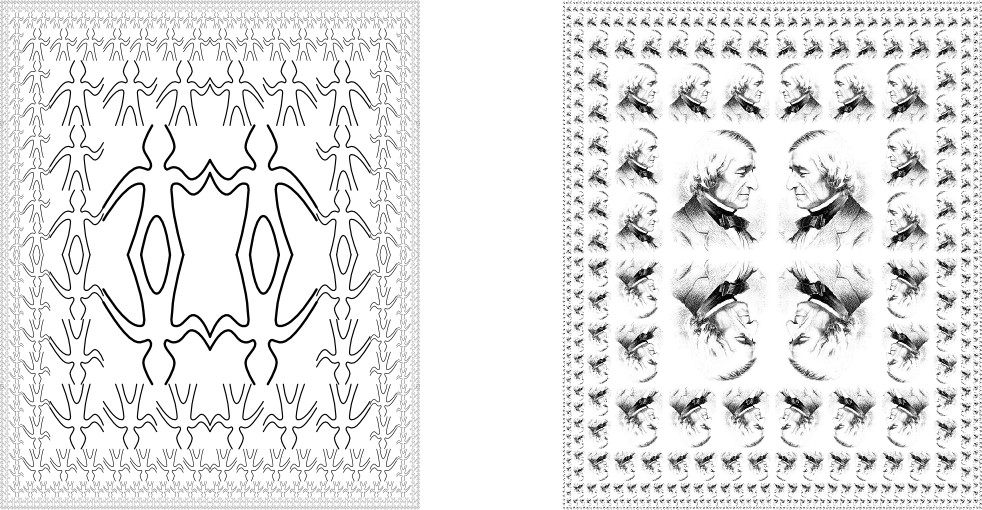
\includegraphics[width=111mm]{fig/chap2/Fig2.9-bigger.png}
	\caption{
		Designs generated with the picture language.
	}
	\label{Figure 2.9}
\end{figure}

\begin{figure}[tb]
	\centering
	\includesvg[width=50mm]{fig/chap2/Fig2.10.svg}
	\caption{
		Images produced by the \code{wave} painter, with respect to four different frames.
		The frames, shown with dotted lines, are not part of the images.
	}
	\label{Figure 2.10}
\end{figure}

Part of the elegance of this picture language is that there is only one kind of element, called a \newterm{painter}.
A painter draws an image that is shifted and scaled to fit within a designated parallelogram-shaped frame.
For example, there’s a primitive painter we’ll call \code{wave} that makes a crude line drawing, as shown in \link{Figure 2.10}.
The actual shape of the drawing depends on the frame---all four images in figure 2.10 are produced by the same \code{wave} painter, but with respect to four different frames.
Painters can be more elaborate than this:
The primitive painter called \code{rogers} paints a picture of \acronym{MIT}’s founder, William Barton Rogers, as shown in \link{Figure 2.11}.%
\footnote{
	William Barton Rogers (1804--1882) was the founder and first president of \acronym{MIT}.
	A geologist and talented teacher, he taught at William and Mary College and at the University of Virginia.
	In 1859 he moved to Boston, where he had more time for research, worked on a plan for establishing a “polytechnic institute,” and served as Massachusetts’s first State Inspector of Gas Meters.

	When \acronym{MIT} was established in 1861, Rogers was elected its first president.
	Rogers espoused an ideal of “useful learning” that was different from the university education of the time, with its overemphasis on the classics, which, as he wrote, “stand in the way of the broader, higher and more practical instruction and discipline of the natural and social sciences.”
	This education was likewise to be different from narrow trade-school education.
	In Rogers’s words:

	\begin{quote}
		The world-enforced distinction between the practical and the scientific worker
		is utterly futile, and the whole experience of modern times has demonstrated
		its utter worthlessness.
	\end{quote}

	Rogers served as president of \acronym{MIT} until 1870, when he resigned due to ill health.
	In 1878 the second president of \acronym{MIT}, John Runkle, resigned under the pressure of a financial crisis brought on by the Panic of 1873 and strain of fighting off attempts by Harvard to take over \acronym{MIT}.
	Rogers returned to hold the office of president until 1881.

	Rogers collapsed and died while addressing \acronym{MIT}’s graduating class at the commencement exercises of 1882.
	Runkle quoted Rogers’s last words in a memorial address delivered that same year:

	\begin{quote}
		“As I stand here today and see what the Institute is, … I call to mind the beginnings of science.
		I remember one hundred and fifty years ago Stephen Hales published a pamphlet on the subject of illuminating gas, in which he stated that his researches had demonstrated that 128 grains of bituminous coal -- ” “Bituminous coal,” these were his last words on earth.
		Here he bent forward, as if consulting some notes on the table before him, then slowly regaining an erect position, threw up his hands, and was translated from the scene of his earthly labors and triumphs to “the tomorrow of death,” where the mysteries of life are solved, and the disembodied spirit finds unending satisfaction in contemplating the new and still unfathomable mysteries of the infinite future.
	\end{quote}

	In the words of Francis A. Walker (\acronym{MIT}’s third president):

	\begin{quote}
		All his life he had borne himself most faithfully and heroically, and he died  as so good a knight would surely have wished, in harness, at his post, and in the very part and act of public duty.
	\end{quote}
}
The four images in figure 2.11 are drawn with respect to the same four frames as the \code{wave} images in figure 2.10.

\begin{figure}[tb]
	\centering
	\includesvg[width=48mm]{fig/chap2/Fig2.11.svg}
	\caption{
		Images of William Barton Rogers, founder and first president of \acronym{MIT}, painted with respect to the same four frames as in \link{Figure 2.10} (original image from Wikimedia Commons).
	}
	\label{Figure 2.11}
\end{figure}

To combine images, we use various operations that construct new painters from given painters.
For example, the \code{beside} operation takes two painters and produces a new, compound painter that draws the first painter’s image in the left half of the frame and the second painter’s image in the right half of the frame.
Similarly, \code{below} takes two painters and produces a compound painter that draws the first painter’s image below the second painter’s image.
Some operations transform a single painter to produce a new painter.
For example, \code{flip-vert} takes a painter and produces a painter that draws its image upside-down, and \code{flip-horiz} produces a painter that draws the original painter’s image left-to-right reversed.

\link{Figure 2.12} shows the drawing of a painter called
\code{wave4} that is built up in two stages starting from \code{wave}:
\begin{scheme}
  (define wave2 (beside wave (flip-vert wave)))
  (define wave4 (below wave2 wave2))
\end{scheme}
\begin{figure}[tb]
	\centering
	\includesvg[width=50mm]{fig/chap2/Fig2.12.svg}
	\caption{
		Creating a complex figure, starting from the \code{wave} painter of \link{Figure 2.10}.
	}
	\label{Figure 2.12}
\end{figure}
In building up a complex image in this manner we are exploiting the fact that painters are closed under the language’s means of combination.
The \code{beside} or \code{below} of two painters is itself a painter;
therefore, we can use it as an element in making more complex painters.
As with building up list structure using \code{cons}, the closure of our data under the means of combination is crucial to the ability to create complex structures while using only a few operations.

Once we can combine painters, we would like to be able to abstract typical  patterns of combining painters.
We will implement the painter operations as Scheme procedures.
This means that we don’t need a special abstraction mechanism in the picture language:
Since the means of combination are ordinary Scheme procedures, we automatically have the capability to do anything with painter operations that we can do with procedures.
For example, we can abstract the pattern in \code{wave4} as 
\begin{scheme}
  (define (flipped-pairs painter)
    (let ((painter2 (beside painter (flip-vert painter))))
      (below painter2 painter2)))
\end{scheme}
and define \code{wave4} as an instance of this pattern:
\begin{scheme}
  (define wave4 (flipped-pairs wave))
\end{scheme}

\begin{figure}[tb]
	\centering
	\includesvg[width=111mm]{fig/chap2/Fig2.13a.svg}
	\caption{
		Recursive plans for \code{right-split} and \code{corner-split}.
	}
	\label{Figure 2.13}
\end{figure}

We can also define recursive operations.  Here’s one that makes painters split
and branch towards the right as shown in \link{Figure 2.13}
and \link{Figure 2.14}:
\begin{scheme}
  (define (right-split painter n)
    (if (= n 0)
        painter
        (let ((smaller (right-split painter (- n 1))))
          (beside painter (below smaller smaller)))))
\end{scheme}
We can produce balanced patterns by branching upwards as well as towards the right (see exercise \link{Exercise 2.44} and figures \link{Figure 2.13} and \link{Figure 2.14}):
\begin{scheme}
  (define (corner-split painter n)
    (if (= n 0)
        painter
        (let ((up (up-split painter (- n 1)))
              (right (right-split painter (- n 1))))
          (let ((top-left (beside up up))
                (bottom-right (below right right))
                (corner (corner-split painter (- n 1))))
            (beside (below painter top-left)
                    (below bottom-right corner))))))
\end{scheme}

By placing four copies of a \code{corner-split} appropriately, we obtain a pattern called \code{square-limit}, whose application to \code{wave} and \code{rogers} is shown in \link{Figure 2.9}:
\begin{scheme}
  (define (square-limit painter n)
    (let ((quarter (corner-split painter n)))
      (let ((half (beside (flip-horiz quarter) quarter)))
        (below (flip-vert half) half))))
\end{scheme}



\begin{exercise}
	\label{Exercise 2.44}
	Define the procedure \code{up-split} used by \code{corner-split}.
	It is similar to \code{right-split}, except that it switches the roles of \code{below} and \code{beside}.
\end{exercise}



\begin{figure}[tbp]
	\centering
	\includesvg[width=91mm]{fig/chap2/Fig2.14b.svg}
	\caption{
		The recursive operations \code{right-split} and \code{corner-split} applied to the painters \code{wave} and \code{rogers}.
		Combining four \code{corner-split} figures produces symmetric \code{square-limit} designs as shown in \link{Figure 2.9}.
	}
	\label{Figure 2.14}
\end{figure}



\subsubsection*{Higher-order operations}

In addition to abstracting patterns of combining painters, we can work at a higher level, abstracting patterns of combining painter operations.
That is, we can view the painter operations as elements to manipulate and can write means of combination for these elements---procedures that take painter operations as arguments and create new painter operations.

For example, \code{flipped-pairs} and \code{square-limit} each arrange four copies of a painter’s image in a square pattern;
they differ only in how they orient the copies.
One way to abstract this pattern of painter combination is with the following procedure, which takes four one-argument painter operations and produces a painter operation that transforms a given painter with those four operations and arranges the results in a square.
\code{tl}, \code{tr}, \code{bl}, and \code{br} are the transformations to apply to the top left copy, the top right copy, the bottom left copy, and the bottom right copy, respectively.
\begin{scheme}
  (define (square-of-four tl tr bl br)
    (lambda (painter)
      (let ((top (beside (tl painter) (tr painter)))
            (bottom (beside (bl painter) (br painter))))
        (below bottom top))))
\end{scheme}
Then \code{flipped-pairs} can be defined in terms of \code{square-of-four} as
follows:%
\footnote{
	Equivalently, we could write
	\begin{smallscheme}
	  (define flipped-pairs
	    (square-of-four identity flip-vert identity flip-vert))
	\end{smallscheme}
}
\begin{scheme}
  (define (flipped-pairs painter)
    (let ((combine4 (square-of-four identity flip-vert
                                    identity flip-vert)))
      (combine4 painter)))
\end{scheme}
and \code{square-limit} can be expressed as%
\footnote{
	\code{rotate180} rotates a painter by \( 180 \) degrees (see \link{Exercise 2.50}).
	Instead of \code{rotate180} we could say \code{(compose flip-vert flip-horiz)}, using the \code{compose} procedure from \link{Exercise 1.42}.
}
\begin{scheme}
  (define (square-limit painter n)
    (let ((combine4 (square-of-four flip-horiz identity
                                    rotate180 flip-vert)))
      (combine4 (corner-split painter n))))
\end{scheme}



\begin{exercise}
	\label{Exercise 2.45}
	\code{right-split} and \code{up-split} can be expressed as instances of a general splitting operation.
	Define a procedure \code{split} with the property that evaluating
	\begin{scheme}
	  (define right-split (split beside below))
	  (define up-split (split below beside))
	\end{scheme}
	produces procedures \code{right-split} and \code{up-split} with the same behaviors as the ones already defined.
\end{exercise}



\subsubsection*{Frames}

Before we can show how to implement painters and their means of combination, we must first consider frames.
A frame can be described by three vectors---an origin vector and two edge vectors.
The origin vector specifies the offset of the frame’s origin from some absolute origin in the plane, and the edge vectors specify the offsets of the frame’s corners from its origin.
If the edges are perpendicular, the frame will be rectangular.
Otherwise the frame will be a more general parallelogram.

\link{Figure 2.15} shows a frame and its associated vectors.
In accordance with data abstraction, we need not be specific yet about how frames are represented, other than to say that there is a constructor \code{make-frame}, which takes three vectors and produces a frame, and three corresponding selectors \code{origin-frame}, \code{edge1-frame}, and \code{edge2-frame} (see \link{Exercise 2.47}).

\begin{figure}[tb]
	\centering
	\includesvg[width=51mm]{fig/chap2/Fig2.15a.svg}
	\caption{
		A frame is described by three vectors --- an origin and two edges.
	}
	\label{Figure 2.15}
\end{figure}

We will use coordinates in the unit square \( (0 ≤ x, y ≤ 1) \) to specify images.
With each frame, we associate a \newterm{frame coordinate map}, which will be used to shift and scale images to fit the frame.
The map transforms the unit square into the frame by mapping the vector \( v = (x, y) \) to the vector sum
\[
	\operatorname{Origin}(\mathrm{Frame})
	+ x ⋅ \operatorname{Edge}_1(\mathrm{Frame})
	+ y ⋅ \operatorname{Edge}_2(\mathrm{Frame}) \,.
\]
For example, \( (0, 0) \) is mapped to the origin of the frame, \( (1, 1) \) to the vertex  diagonally opposite the origin, and \( (0.5, 0.5) \) to the center of the frame.
We can create a frame’s coordinate map with the following procedure:%
\footnote{
	\code{frame-coord-map} uses the vector operations described in \link{Exercise 2.46} below, which we assume have been implemented using some representation for vectors.
	Because of data abstraction, it doesn’t matter what this vector representation is, so long as the vector operations behave correctly.
}
\begin{scheme}
  (define (frame-coord-map frame)
    (lambda (v)
      (add-vect
       (origin-frame frame)
       (add-vect (scale-vect (xcor-vect v) (edge1-frame frame))
                 (scale-vect (ycor-vect v) (edge2-frame frame))))))
\end{scheme}
Observe that applying \code{frame-coord-map} to a frame returns a procedure that, given a vector, returns a vector.
If the argument vector is in the unit square, the result vector will be in the frame.
For example,
\begin{scheme}
  ((frame-coord-map a-frame) (make-vect 0 0))
\end{scheme}
returns the same vector as
\begin{scheme}
  (origin-frame a-frame)
\end{scheme}



\begin{exercise}
	\label{Exercise 2.46}
	A two-dimensional vector \( v \) running from the origin to a point can be represented as a pair consisting of an \( x \)-coordinate and a \( y \)-coordinate.
	Implement a data abstraction for vectors by giving a constructor \code{make-vect} and corresponding selectors \code{xcor-vect} and \code{ycor-vect}.
	In terms of your selectors and constructor, implement procedures \code{add-vect}, \code{sub-vect}, and \code{scale-vect} that perform the operations vector addition, vector subtraction, and multiplying a vector by a scalar:
	\begin{align*}
		(x_1, y_1) + (x_2, y_2) &= (x_1 + x_2, y_1 + y_2) \,, \\
		(x_1, y_1) - (x_2, y_2) &= (x_1 - x_2, y_1 - y_2) \,, \\
		s ⋅ (x, y)              &= (s x, s y) \,.
	\end{align*}
\end{exercise}



\begin{exercise}
	\label{Exercise 2.47}
	Here are two possible constructors for frames:
	\begin{scheme}
	  (define (make-frame origin edge1 edge2)
	    (list origin edge1 edge2))

	  (define (make-frame origin edge1 edge2)
	    (cons origin (cons edge1 edge2)))
	\end{scheme}
	For each constructor supply the appropriate selectors to produce an implementation for frames.
\end{exercise}



\subsubsection*{Painters}

A painter is represented as a procedure that, given a frame as argument, draws a particular image shifted and scaled to fit the frame.
That is to say, if \code{p} is a painter and \code{f} is a frame, then we produce \code{p}’s image in \code{f} by calling \code{p} with \code{f} as argument.

The details of how primitive painters are implemented depend on the particular characteristics of the graphics system and the type of image to be drawn.
For instance, suppose we have a procedure \code{draw-line} that draws a line on the screen between two specified points.
Then we can create painters for line drawings, such as the \code{wave} painter in \link{Figure 2.10}, from lists of line segments as follows:%
\footnote{
	\code{segments->painter} uses the representation for line segments described in \link{Exercise 2.48} below.
	It also uses the \code{for-each} procedure described in \link{Exercise 2.23}.
}
\begin{scheme}
  (define (segments->painter segment-list)
    (lambda (frame)
      (for-each
       (lambda (segment)
         (draw-line
          ((frame-coord-map frame)
           (start-segment segment))
          ((frame-coord-map frame)
           (end-segment segment))))
       segment-list)))
\end{scheme}
The segments are given using coordinates with respect to the unit square.
For each segment in the list, the painter transforms the segment endpoints with the frame coordinate map and draws a line between the transformed points.

Representing painters as procedures erects a powerful abstraction barrier in the picture language.
We can create and intermix all sorts of primitive painters, based on a variety of graphics capabilities.
The details of their implementation do not matter.
Any procedure can serve as a painter, provided that it takes a frame as argument and draws something scaled to fit the frame.%
\footnote{
	For example, the \code{rogers} painter of \link{Figure 2.11} was constructed from a gray-level image.
	For each point in a given frame, the \code{rogers} painter determines the point in the image that is mapped to it under the frame coordinate map, and shades it accordingly.
	By allowing different types of painters, we are capitalizing on the abstract data idea discussed in \link{Section 2.1.3}, where we argued that a rational-number representation could be anything at all that satisfies an appropriate condition.
	Here we’re using the fact that a painter can be implemented in any way at all, so long as it draws something in the designated frame.
	\link{Section 2.1.3} also showed how pairs could be implemented as procedures.
	Painters are our second example of a procedural representation for data.
}



\begin{exercise}
	\label{Exercise 2.48}
	A directed line segment in the plane can be represented as a pair of vectors---the vector running from the origin to the start-point of the segment, and the vector running from the origin to the end-point of the segment.
	Use your vector representation from \link{Exercise 2.46} to define a representation for segments with a constructor \code{make-segment} and selectors \code{start-segment} and \code{end-segment}.
\end{exercise}



\begin{exercise}
	\label{Exercise 2.49}
	Use \code{segments->painter} to define the following primitive painters:
	\begin{enumerate}[label = \alph*., leftmargin = *]

		\item
			The painter that draws the outline of the designated frame.

		\item
			The painter that draws an “X” by connecting opposite corners of the frame.

		\item
			The painter that draws a diamond shape by connecting the midpoints of the sides of the frame.

		\item
			The \code{wave} painter.

	\end{enumerate}
\end{exercise}



\subsubsection*{Transforming and combining painters}

An operation on painters (such as \code{flip-vert} or \code{beside}) works by creating a painter that invokes the original painters with respect to frames derived from the argument frame.
Thus, for example, \code{flip-vert} doesn’t have to know how a painter works in order to flip it---it just has to know how to turn a frame upside down:
The flipped painter just uses the original painter, but in the inverted frame.

Painter operations are based on the procedure \code{transform-painter}, which takes as arguments a painter and information on how to transform a frame and produces a new painter.
The transformed painter, when called on a frame, transforms the frame and calls the original painter on the transformed frame.
The arguments to \code{transform-painter} are points (represented as vectors) that specify the corners of the new frame:
When mapped into the frame, the first point specifies the new frame’s origin and the other two specify the ends of its edge vectors.
Thus, arguments within the unit square specify a frame contained within the original frame.
\begin{scheme}
  (define (transform-painter painter origin corner1 corner2)
    (lambda (frame)
      (let ((m (frame-coord-map frame)))
        (let ((new-origin (m origin)))
          (painter (make-frame
                    new-origin
                    (sub-vect (m corner1) new-origin)
                    (sub-vect (m corner2) new-origin)))))))
\end{scheme}

Here’s how to flip painter images vertically:
\begin{scheme}
  (define (flip-vert painter)
    (transform-painter painter
                       (make-vect 0.0 1.0)   ~\textrm{; new \code{origin}}~
                       (make-vect 1.0 1.0)   ~\textrm{; new end of \code{edge1}}~
                       (make-vect 0.0 0.0))) ~\textrm{; new end of \code{edge2}}~
\end{scheme}
Using \code{transform-painter}, we can easily define new transformations.
For example, we can define a painter that shrinks its image to the upper-right quarter of the frame it is given:
\begin{scheme}
  (define (shrink-to-upper-right painter)
    (transform-painter
     painter (make-vect 0.5 0.5)
     (make-vect 1.0 0.5) (make-vect 0.5 1.0)))
\end{scheme}
Other transformations rotate images counterclockwise by 90 degrees%
\footnote{
	\code{rotate90} is a pure rotation only for square frames, because it also stretches and shrinks the image to fit into the rotated frame.
}
\begin{scheme}
  (define (rotate90 painter)
    (transform-painter painter
                       (make-vect 1.0 0.0)
                       (make-vect 1.0 1.0)
                       (make-vect 0.0 0.0)))
\end{scheme}
or squash images towards the center of the frame:%
\footnote{
	The diamond-shaped images in \link{Figure 2.10} and \link{Figure 2.11} were created with \code{squash-inwards} applied to \code{wave} and \code{rogers}.
}
\begin{scheme}
  (define (squash-inwards painter)
    (transform-painter painter
                       (make-vect 0.0 0.0)
                       (make-vect 0.65 0.35)
                       (make-vect 0.35 0.65)))
\end{scheme}

Frame transformation is also the key to defining means of combining two or more painters.
The \code{beside} procedure, for example, takes two painters, transforms them to paint in the left and right halves of an argument frame respectively, and produces a new, compound painter.
When the compound painter is given a frame, it calls the first transformed painter to paint in the left half of the frame and calls the second transformed painter to paint in the right half of the frame:
\begin{scheme}
  (define (beside painter1 painter2)
    (let ((split-point (make-vect 0.5 0.0)))
      (let ((paint-left
             (transform-painter
              painter1
              (make-vect 0.0 0.0)
              split-point
              (make-vect 0.0 1.0)))
            (paint-right
             (transform-painter
              painter2
              split-point
              (make-vect 1.0 0.0)
              (make-vect 0.5 1.0))))
        (lambda (frame)
          (paint-left frame)
          (paint-right frame)))))
\end{scheme}

Observe how the painter data abstraction, and in particular the representation of painters as procedures, makes \code{beside} easy to implement.
The \code{beside} procedure need not know anything about the details of the component painters other than that each painter will draw something in its designated frame.

\begin{exercise}
\label{Exercise 2.50}
Define the transformation \code{flip-horiz}, which flips painters horizontally, and transformations that rotate painters counterclockwise by \( 180 \) degrees and \( 270 \) degrees.
\end{exercise}



\begin{exercise}
\label{Exercise 2.51}
Define the \code{below} operation for painters.
\code{below} takes two painters as arguments.
The resulting painter, given a frame, draws with the first painter in the bottom of the frame and with the second painter in the top.
Define \code{below} in two different ways---first by writing a procedure that is analogous to the \code{beside} procedure given above, and again in terms of \code{beside} and suitable rotation operations (from \link{Exercise 2.50}).
\end{exercise}



\subsubsection*{Levels of language for robust design}

The picture language exercises some of the critical ideas we’ve introduced about abstraction with procedures and data.
The fundamental data abstractions, painters, are implemented using procedural representations, which enables the language to handle different basic drawing capabilities in a uniform way.
The means of combination satisfy the closure property, which permits us to easily build up complex designs.
Finally, all the tools for abstracting procedures are available to us for abstracting means of combination for painters.

We have also obtained a glimpse of another crucial idea about languages and program design.
This is the approach of \newterm{stratified design}, the notion that a complex system should be structured as a sequence of levels that are described using a sequence of languages.
Each level is constructed by combining parts that are regarded as primitive at that level, and the parts constructed at each level are used as primitives at the next level.
The language used at each level of a stratified design has primitives, means of combination, and means of abstraction appropriate to that level of detail.

Stratified design pervades the engineering of complex systems.
For example, in computer engineering, resistors and transistors are combined (and described using a language of analog circuits) to produce parts such as and-gates and or-gates, which form the primitives of a language for digital-circuit design.%
\footnote{
	\link{Section 3.3.4} describes one such language.
}
These parts are combined to build processors, bus structures, and memory systems, which are in turn combined to form computers, using languages appropriate to computer architecture.
Computers are combined to form distributed systems, using languages appropriate for describing network interconnections, and so on.

As a tiny example of stratification, our picture language uses primitive elements (primitive painters) that are created using a language that specifies points and lines to provide the lists of line segments for \code{segments->painter}, or the shading details for a painter like \code{rogers}.
The bulk of our description of the picture language focused on combining these primitives, using geometric combiners such as \code{beside} and \code{below}.
We also worked at a higher level, regarding \code{beside} and \code{below} as primitives to be manipulated in a language whose operations, such as \code{square-of-four}, capture common patterns of combining geometric combiners.

Stratified design helps make programs \newterm{robust}, that is, it makes it likely that small changes in a specification will require correspondingly small changes in the program.
For instance, suppose we wanted to change the image based on \code{wave} shown in \link{Figure 2.9}.
We could work at the lowest level to change the detailed appearance of the \code{wave} element;
we could work at the middle level to change the way \code{corner-split} replicates the \code{wave};
we could work at the highest level to change how \code{square-limit} arranges the four copies of the corner.
In general, each level of a stratified design provides a different vocabulary for expressing the characteristics of the system, and a different kind of ability to change it.



\begin{exercise}
	\label{Exercise 2.52}
	Make changes to the square limit of \code{wave} shown in \link{Figure 2.9} by working at each of the levels described above.
	In particular:
	\begin{enumerate}[label = \alph*., leftmargin = *]

		\item
			Add some segments to the primitive \code{wave} painter of \link{Exercise 2.49} (to add a smile, for example).

		\item
			Change the pattern constructed by \code{corner-split} (for example, by using only one copy of the \code{up-split} and \code{right-split} images instead of two).

		\item
			Modify the version of \code{square-limit} that uses \code{square-of-four} so as to assemble the corners in a different pattern.
			(For example, you might make the big Mr.~Rogers look outward from each corner of the square.)

	\end{enumerate}
\end{exercise}

\section{Symbolic Data}
\label{Section 2.3}

All the compound data objects we have used so far were constructed ultimately from numbers.
In this section we extend the representational capability of our language by introducing the ability to work with arbitrary symbols as data.



\subsection{Quotation}
\label{Section 2.3.1}

If we can form compound data using symbols, we can have lists such as
\begin{scheme}
  (a b c d)
  (23 45 17)
  ((Norah 12) (Molly 9) (Anna 7) (Lauren 6) (Charlotte 4))
\end{scheme}
Lists containing symbols can look just like the expressions of our  language:

\begin{scheme}
  (* (+ 23 45)
     (+ x 9))

  (define (fact n)
    (if (= n 1) 1 (* n (fact (- n 1)))))
\end{scheme}

In order to manipulate symbols we need a new element in our language:
the ability to \newterm{quote} a data object.
Suppose we want to construct the list \code{(a b)}.
We can’t accomplish this with \code{(list a b)}, because this expression constructs a list of the \newterm{values} of \code{a} and \code{b} rather than the symbols themselves.
This issue is well known in the context of natural languages, where words and sentences may be regarded either as semantic entities or as character strings (syntactic entities).
The common practice in natural languages is to use quotation marks to indicate that a word or a sentence is to be treated literally as a string of characters.
For instance, the first letter of “John”  is clearly  “J.”
If we tell somebody “say your name aloud,” we expect to hear that person’s name.
However, if we tell somebody “say ‘your name’ aloud,” we expect to hear the words “your name.”
Note that we are forced to nest quotation marks to describe what somebody else might say.%
\footnote{
	Allowing quotation in a language wreaks havoc with the ability to reason about the language in simple terms, because it destroys the notion that equals can be substituted for equals.
	For example, three is one plus two, but the word “three” is not the phrase “one plus two.”
	Quotation is powerful because it gives us a way to build expressions that manipulate other expressions (as we will see when we write an interpreter in \link{Chapter 4}).
	But allowing statements in a language that talk about other statements in that language makes it very difficult to maintain any coherent principle of what “equals can be substituted for equals” should mean.
	For example, if we know that the evening star is the morning star, then from the statement “the evening star is Venus” we can deduce “the morning star is Venus.”
	However, given that  “John knows that the evening star is Venus” we cannot infer that “John knows that the morning star is Venus.”
}

We can follow this same practice to identify lists and symbols that are to be treated as data objects rather than as expressions to be evaluated.
However, our format for quoting differs from that of natural languages in that we place a quotation mark (traditionally, the single quote symbol \code{'}) only at the beginning of the object to be quoted.
We can get away with this in Scheme syntax because we rely on blanks and parentheses to delimit objects.
Thus, the meaning of the single quote character is to quote the next object.%
\footnote{
	The single quote is different from the double quote we have been using to enclose character strings to be printed.
	Whereas the single quote can be used to denote lists or symbols, the double quote is used only with character strings.
	In this book, the only use for character strings is as items to be printed.
}

Now we can distinguish between symbols and their values:

\begin{scheme}
  (define a 1)

  (define b 2)

  (list a b)
  ~\outprint{(1 2)}~

  (list 'a 'b)
  ~\outprint{(a b)}~

  (list 'a b)
  ~\outprint{(a 2)}~
\end{scheme}

Quotation also allows us to type in compound objects, using the conventional printed representation for lists:%
\footnote{
	Strictly, our use of the quotation mark violates the general rule that all compound expressions in our language should be delimited by parentheses and look like lists.
	We can recover this consistency by introducing a special form \code{quote}, which serves the same purpose as the quotation mark.
	Thus, we would type \code{(quote a)} instead of \code{'a}, and we would type \code{(quote (a b c))} instead of \code{'(a b c)}.
	This is precisely how the interpreter works.
	The quotation mark is just a single-character abbreviation for wrapping the next complete expression with \code{quote} to form \code{(quote ⟨\var{expression}⟩)}.
	This is important because it maintains the principle that any expression seen by the interpreter can be manipulated as a data object.
	For instance, we could construct the expression \code{(car '(a b c))}, which is the same as \code{(car (quote (a b c)))}, by evaluating \code{(list 'car (list 'quote '(a b c)))}.
}
\begin{scheme}
  (car '(a b c))
  ~\outprint{a}~

  (cdr '(a b c))
  ~\outprint{(b c)}~
\end{scheme}
In keeping with this, we can obtain the empty list by evaluating \code{'()}, and thus dispense with the variable \code{nil}.

One additional primitive used in manipulating symbols is \code{eq?}, which takes two symbols as arguments and tests whether they are the same.%
\footnote{
	We can consider two symbols to be “the same” if they consist of the same characters in the same order.
	Such a definition skirts a deep issue that we are not yet ready to address:
	the meaning of “sameness” in a programming language.
	We will return to this in \link{Chapter 3} (\link{Section 3.1.3}).
}
Using \code{eq?}, we can implement a useful procedure called \code{memq}.
This takes two arguments, a symbol and a list.
If the symbol is not contained in the list (i.e., is not \code{eq?} to any item in the list), then \code{memq} returns false.
Otherwise, it returns the sublist of the list beginning with the first occurrence of the symbol:
\begin{scheme}
  (define (memq item x)
    (cond ((null? x) false)
          ((eq? item (car x)) x)
          (else (memq item (cdr x)))))
\end{scheme}
For example, the value of
\begin{scheme}
  (memq 'apple '(pear banana prune))
\end{scheme}
is false, whereas the value of
\begin{scheme}
  (memq 'apple '(x (apple sauce) y apple pear))
\end{scheme}
is \code{(apple pear)}.



\begin{exercise}
	\label{Exercise 2.53}
	What would the interpreter print in response to evaluating each of the following expressions?
	\begin{scheme}
	  (list 'a 'b 'c)

	  (list (list 'george))

	  (cdr '((x1 x2) (y1 y2)))

	  (cadr '((x1 x2) (y1 y2)))

	  (pair? (car '(a short list)))

	  (memq 'red '((red shoes) (blue socks)))

	  (memq 'red '(red shoes blue socks))
	\end{scheme}
\end{exercise}



\begin{exercise}
	\label{Exercise 2.54}
	Two lists are said to be \code{equal?} if they contain equal elements arranged in the same order.
	For example,
	\begin{scheme}
	  (equal? '(this is a list) '(this is a list))
	\end{scheme}
	is true, but
	\begin{scheme}
	  (equal? '(this is a list) '(this (is a) list))
	\end{scheme}
	is false.
	To be more precise, we can define \code{equal?}  recursively in terms of the basic \code{eq?} equality of symbols by saying that \code{a} and \code{b} are \code{equal?} if they are both symbols and the symbols are \code{eq?}, or if they are both lists such that \code{(car a)} is \code{equal?} to \code{(car b)} and \code{(cdr a)} is \code{equal?} to \code{(cdr b)}.
	Using this idea, implement \code{equal?} as a procedure.%
	\footnote{
		In practice, programmers use \code{equal?} to compare lists that contain numbers as well as symbols.
		Numbers are not considered to be symbols.
		The question of whether two numerically equal numbers (as tested by \code{=}) are also \code{eq?} is highly implementation-dependent.
		A better definition of \code{equal?} (such as the one that comes as a primitive in Scheme) would also stipulate that if \code{a} and \code{b} are both numbers, then \code{a} and \code{b} are \code{equal?} if they are numerically equal.
	}
\end{exercise}



\begin{exercise}
	\label{Exercise 2.55}
	Eva Lu Ator types to the interpreter the expression
	\begin{scheme}
	  (car ''abracadabra)
	\end{scheme}
	To her surprise, the interpreter prints back \code{quote}.
	Explain.
\end{exercise}



\subsection{Example: Symbolic Differentiation}
\label{Section 2.3.2}

As an illustration of symbol manipulation and a further illustration of data abstraction, consider the design of a procedure that performs symbolic differentiation of algebraic expressions.
We would like the procedure to take as arguments an algebraic expression and a variable and to return the derivative of the expression with respect to the variable.
For example, if the arguments to the procedure are \( a x^2 + b x + c \) and \( x \), the procedure should return \( 2a x + b \).
Symbolic differentiation is of special historical significance in Lisp.
It was one of the motivating examples behind the development of a computer language for symbol manipulation.
Furthermore, it marked the beginning of the line of research that led to the development of powerful systems for symbolic mathematical work, which are currently being used by a growing number of applied mathematicians and physicists.

In developing the symbolic-differentiation program, we will follow the same strategy of data abstraction that we followed in developing the rational-number system of \link{Section 2.1.1}.
That is, we will first define a differentiation algorithm that operates on abstract objects such as “sums,” “products,” and “variables” without worrying about how these are to be represented.
Only afterward will we address the representation problem.



\subsubsection*{The differentiation program with abstract data}

In order to keep things simple, we will consider a very simple symbolic-differentiation program that handles expressions that are built up using only the operations of addition and multiplication with two arguments.
Differentiation of any such expression can be carried out by applying the following reduction rules:
\begin{itemize}

	\item
		\( \frac{dc}{dx} = 0 \) for \( c \) a constant or a variable different from \( x \),

	\item
		\( \frac{dx}{dx} = 1 \),

	\item
		\( \frac{d(u + v)}{dx} = \frac{du}{dx} + \frac{dv}{dx} \),

	\item
		\( \frac{d(uv)}{dx} = u \Bigl( \frac{dv}{dx} \Bigr) + v \Bigl( \frac{du}{dx} \Bigr) \).
\end{itemize}

Observe that the latter two rules are recursive in nature.
That is, to obtain the derivative of a sum we first find the derivatives of the terms and add them.
Each of the terms may in turn be an expression that needs to be decomposed.
Decomposing into smaller and smaller pieces will eventually produce pieces that are either constants or variables, whose derivatives will be either \( 0 \) or \( 1 \).

To embody these rules in a procedure we indulge in a little wishful thinking, as we did in designing the rational-number implementation.
If we had a means for representing algebraic expressions, we should be able to tell whether an expression is a sum, a product, a constant, or a variable.
We should be able to extract the parts of an expression.
For a sum, for example we want to be able to extract the addend (first term) and the augend (second term).
We should also be able to construct expressions from parts.
Let us assume that we already have procedures to implement the following selectors, constructors, and predicates:

\begin{scheme}
  (variable? e)            ~\textrm{Is \code{e} a variable?}~
  (same-variable? v1 v2)   ~\textrm{Are \code{v1} and \code{v2} the same variable?}~

  (sum? e)                 ~\textrm{Is \code{e} a sum?}~
  (addend e)               ~\textrm{Addend of the sum \code{e}.}~
  (augend e)               ~\textrm{Augend of the sum \code{e}.}~
  (make-sum a1 a2)         ~\textrm{Construct the sum of \code{a1} and \code{a2}.}~

  (product? e)             ~\textrm{Is \code{e} a product?}~
  (multiplier e)           ~\textrm{Multiplier of the product \code{e}.}~
  (multiplicand e)         ~\textrm{Multiplicand of the product \code{e}.}~
  (make-product m1 m2)     ~\textrm{Construct the product of \code{m1} and \code{m2}.}~
\end{scheme}
Using these, and the primitive predicate \code{number?}, which identifies numbers, we can express the differentiation rules as the following procedure:
\begin{scheme}
  (define (deriv exp var)
    (cond ((number? exp) 0)
          ((variable? exp) (if (same-variable? exp var) 1 0))
          ((sum? exp) (make-sum (deriv (addend exp) var)
                                (deriv (augend exp) var)))
          ((product? exp)
           (make-sum
             (make-product (multiplier exp)
                           (deriv (multiplicand exp) var))
             (make-product (deriv (multiplier exp) var)
                           (multiplicand exp))))
          (else
           (error "unknown expression type: DERIV" exp))))
\end{scheme}
This \code{deriv} procedure incorporates the complete differentiation algorithm.
Since it is expressed in terms of abstract data, it will work no matter how we choose to represent algebraic expressions, as long as we design a proper set of selectors and constructors.
This is the issue we must address next.



\subsubsection*{Representing algebraic expressions}

We can imagine many ways to use list structure to represent algebraic expressions.
For example, we could use lists of symbols that mirror the usual algebraic notation, representing \( a x + b \) as the list \code{(a * x + b)}.
However, one especially straightforward choice is to use the same parenthesized prefix notation that Lisp uses for combinations;
that is, to represent \( a x + b \) as \code{(+ (* a x) b)}.
Then our data representation for the differentiation problem is as follows:

\begin{itemize}

	\item
		The variables are symbols.
		They are identified by the primitive predicate \code{symbol?}:
		\begin{scheme}
		  (define (variable? x) (symbol? x))
		\end{scheme}

	\item
		Two variables are the same if the symbols representing them are \code{eq?}:
		\begin{scheme}
		  (define (same-variable? v1 v2)
		    (and (variable? v1) (variable? v2) (eq? v1 v2)))
		\end{scheme}

	\item
		Sums and products are constructed as lists:
		\begin{scheme}
		  (define (make-sum a1 a2) (list '+ a1 a2))
		  (define (make-product m1 m2) (list '* m1 m2))
		\end{scheme}

	\item
		A sum is a list whose first element is the symbol \code{+}:
		\begin{scheme}
		  (define (sum? x) (and (pair? x) (eq? (car x) '+)))
		\end{scheme}

	\item
		The addend is the second item of the sum list:
		\begin{scheme}
		  (define (addend s) (cadr s))
		\end{scheme}

	\item
		The augend is the third item of the sum list:
		\begin{scheme}
		  (define (augend s) (caddr s))
		\end{scheme}

	\item
		A product is a list whose first element is the symbol \code{*}:
		\begin{scheme}
		  (define (product? x) (and (pair? x) (eq? (car x) '*)))
		\end{scheme}

	\item
		The multiplier is the second item of the product list:
		\begin{scheme}
		  (define (multiplier p) (cadr p))
		\end{scheme}

	\item
		The multiplicand is the third item of the product list:
		\begin{scheme}
		  (define (multiplicand p) (caddr p))
		\end{scheme}

\end{itemize}
Thus, we need only combine these with the algorithm as embodied by \code{deriv} in order to have a working symbolic-differentiation program.
Let us look at some examples of its behavior:
\begin{scheme}
  (deriv '(+ x 3) 'x)
  ~\outprint{(+ 1 0)}~

  (deriv '(* x y) 'x)
  ~\outprint{(+ (* x 0) (* 1 y))}~

  (deriv '(* (* x y) (+ x 3)) 'x)
  ~\outprint{(+ (* (* x y) (+ 1 0))}~
     ~\outprint{(* (+ (* x 0) (* 1 y))}~
        ~\outprint{(+  x 3)))}~
\end{scheme}
The program produces answers that are correct;
however, they are unsimplified.
It is true that
\[
	\frac{d(xy)}{x} = x ⋅ 0 + 1 ⋅ y
\]
but we would like the program to know that \( x ⋅ 0 = 0 \), \( 1 ⋅ y = y \), and \( 0 + y = y \).
The answer for the second example should have been simply \code{y}.
As the third example shows, this becomes a serious issue when the expressions are complex.

Our difficulty is much like the one we encountered with the rational-number implementation:
we haven’t reduced answers to simplest form.
To accomplish the rational-number reduction, we needed to change only the constructors and the selectors of the implementation.
We can adopt a similar strategy here.
We won’t change \code{deriv} at all.
Instead, we will change \code{make-sum} so that if both summands are numbers, \code{make-sum} will add them and return their sum.
Also, if one of the summands is 0, then \code{make-sum} will return the other summand.
\begin{scheme}
  (define (make-sum a1 a2)
    (cond ((=number? a1 0) a2)
          ((=number? a2 0) a1)
          ((and (number? a1) (number? a2))
           (+ a1 a2))
          (else (list '+ a1 a2))))
\end{scheme}
This uses the procedure \code{=number?}, which checks whether an expression is equal to a given number:
\begin{scheme}
  (define (=number? exp num) (and (number? exp) (= exp num)))
\end{scheme}
Similarly, we will change \code{make-product} to build in the rules that \( 0 \) times anything is \( 0 \) and \( 1 \) times anything is the thing itself:
\begin{scheme}
  (define (make-product m1 m2)
    (cond ((or (=number? m1 0) (=number? m2 0)) 0)
          ((=number? m1 1) m2)
          ((=number? m2 1) m1)
          ((and (number? m1) (number? m2)) (* m1 m2))
          (else (list '* m1 m2))))
\end{scheme}
Here is how this version works on our three examples:
\begin{scheme}
  (deriv '(+ x 3) 'x)
  ~\outprint{1}~

  (deriv '(* x y) 'x)
  ~\outprint{y}~

  (deriv '(* (* x y) (+ x 3)) 'x)
  ~\outprint{(+ (* x y) (* y (+ x 3)))}~
\end{scheme}
Although this is quite an improvement, the third example shows that there is still a long way to go before we get a program that puts expressions into a form that we might agree is “simplest.”
The problem of algebraic simplification is complex because, among other reasons, a form that may be simplest for one purpose may not be for another.



\begin{exercise}
	\label{Exercise 2.56}
	Show how to extend the basic differentiator to handle more kinds of expressions.
	For instance, implement the differentiation rule
	\[
		\frac{d(u^n)}{dx} = n u^{n-1} \Bigl( \frac{du}{dx} \Bigr)
	\]
	by adding a new clause to the \code{deriv} program and defining appropriate procedures \code{exponentiation?}, \code{base}, \code{exponent}, and \code{make-exponentiation}.
	(You may use the symbol \code{**} to denote exponentiation.)
	Build in the rules that anything raised to the power \( 0 \) is \( 1 \) and anything raised to the power \( 1 \) is the thing itself.
\end{exercise}



\begin{exercise}
	\label{Exercise 2.57}
	Extend the differentiation program to handle sums and products of arbitrary numbers of (two or more) terms.
	Then the last example above could be expressed as
	\begin{scheme}
	  (deriv '(* x y (+ x 3)) 'x)
	\end{scheme}
	Try to do this by changing only the representation for sums and products, without changing the \code{deriv} procedure at all.
	For example, the \code{addend} of a sum would be the first term, and the \code{augend} would be the sum of the rest of the terms.
\end{exercise}



\begin{exercise}
	\label{Exercise 2.58}
	Suppose we want to modify the differentiation program so that it works with ordinary mathematical notation, in which \code{+} and \code{*} are infix rather than prefix operators.
	Since the differentiation program is defined in terms of abstract data, we can modify it to work with different representations of expressions solely by changing the predicates, selectors, and constructors that define the representation of the algebraic expressions on which the differentiator is to operate.
	\begin{enumerate}[label = \alph*., leftmargin = *]

		\item
			Show how to do this in order to differentiate algebraic expressions presented  in infix form, such as \code{(x + (3 * (x + (y + 2))))}.
			To simplify the task, assume that \code{+} and \code{*} always take two arguments and that expressions are fully parenthesized.

		\item
			The problem becomes substantially harder if we allow standard algebraic notation, such as \code{(x + 3 * (x + y + 2))}, which drops unnecessary parentheses and assumes that multiplication is done before addition.
			Can you design appropriate predicates, selectors, and constructors for this notation such that our derivative program still works?

	\end{enumerate}
\end{exercise}



\subsection{Example: Representing Sets}
\label{Section 2.3.3}

In the previous examples we built representations for two kinds of compound data objects:
rational numbers and algebraic expressions.
In one of these examples we had the choice of simplifying (reducing) the expressions at either construction time or selection time, but other than that the choice of a representation for these structures in terms of lists was straightforward.
When we turn to the representation of sets, the choice of a representation is not so obvious.
Indeed, there are a number of possible representations, and they differ significantly from one another in several ways.

Informally, a set is simply a collection of distinct objects.  To give a more
precise definition we can employ the method of data abstraction.  That is, we
define “set” by specifying the operations that are to be used on sets.  These
are \code{union-set}, \code{intersection-set}, \code{element-of-set?}, and
\code{adjoin-set}.  \code{element-of-set?} is a predicate that determines
whether a given element is a member of a set.  \code{adjoin-set} takes an
object and a set as arguments and returns a set that contains the elements of
the original set and also the adjoined element.  \code{union-set} computes the
union of two sets, which is the set containing each element that appears in
either argument.  \code{intersection-set} computes the intersection of two
sets, which is the set containing only elements that appear in both arguments.
From the viewpoint of data abstraction, we are free to design any
representation that implements these operations in a way consistent with the
interpretations given above.%
\footnote{
	If we want to be more formal, we can specify “consistent with the interpretations given above” to mean that the operations satisfy a collection of rules such as these:
	\begin{itemize}

		\item
			For any set \code{S} and any object \code{x},  \code{(element-of-set? x (adjoin-set x S))} is true (informally:
			“Adjoining an object to a set produces a set that contains the object”).

		\item
			For any sets \code{S} and \code{T} and any object \code{x}, \code{(element-of-set? x (union-set S T))} is equal to \code{(or (element-of-set? x S) (element-of-set? x T))} 
			(informally: “The elements of \code{(union S T)} are the elements that are in \code{S} or in \code{T}”).

		\item
			For any object \code{x}, \code{(element-of-set? x '())} is false
			(informally: “No object is an element of the empty set”).
	\end{itemize}
}



\subsubsection*{Sets as unordered lists}

One way to represent a set is as a list of its elements in which no element appears more than once.
The empty set is represented by the empty list.
In this representation, \code{element-of-set?} is similar to the procedure \code{memq} of \link{Section 2.3.1}.
It uses \code{equal?}  instead of \code{eq?} so that the set elements need not be symbols:
\begin{scheme}
  (define (element-of-set? x set)
    (cond ((null? set) false)
          ((equal? x (car set)) true)
          (else (element-of-set? x (cdr set)))))
\end{scheme}
Using this, we can write \code{adjoin-set}.
If the object to be adjoined is already in the set, we just return the set.
Otherwise, we use \code{cons} to add the object to the list that represents the set:
\begin{scheme}
  (define (adjoin-set x set)
    (if (element-of-set? x set)
        set
        (cons x set)))
\end{scheme}
For \code{intersection-set} we can use a recursive strategy.
If we know how to form the intersection of \code{set2} and the \code{cdr} of \code{set1}, we only need to decide whether to include the \code{car} of \code{set1} in this.
But this depends on whether \code{(car set1)} is also in \code{set2}.
Here is the resulting procedure:
\begin{scheme}
  (define (intersection-set set1 set2)
    (cond ((or (null? set1) (null? set2)) '())
          ((element-of-set? (car set1) set2)
           (cons (car set1) (intersection-set (cdr set1) set2)))
          (else (intersection-set (cdr set1) set2))))
\end{scheme}

In designing a representation, one of the issues we should be concerned with is efficiency.
Consider the number of steps required by our set operations.
Since they all use \code{element-of-set?}, the speed of this operation has a major impact on the efficiency of the set implementation as a whole.
Now, in order to check whether an object is a member of a set, \code{element-of-set?} may have to scan the entire set.
(In the worst case, the object turns out not to be in the set.)
Hence, if the set has \( n \) elements, \code{element-of-set?}  might take up to \( n \) steps.
Thus, the number of steps required grows as \( Θ(n) \).
The number of steps required by \code{adjoin-set}, which uses this operation, also grows as \( Θ(n) \).
For \code{intersection-set}, which does an \code{element-of-set?} check for each element of \code{set1}, the number of steps required grows as the product of the sizes of the sets involved, or \( Θ(n^2) \) for two sets of size \( n \).
The same will be true of \code{union-set}.



\begin{exercise}
	\label{Exercise 2.59}
	Implement the \code{union-set} operation for the unordered-list representation of sets.
\end{exercise}



\begin{exercise}
	\label{Exercise 2.60}
	We specified that a set would be represented as a list with no duplicates.
	Now suppose we allow duplicates.
	For instance, the set \( \{1, 2, 3\} \) could be represented as the list \code{(2 3 2 1 3 2 2)}.
	Design procedures \code{element-of-set?}, \code{adjoin-set}, \code{union-set}, and \code{intersection-set} that operate on this representation.
	How does the efficiency of each compare with the corresponding procedure for the non-duplicate representation?
	Are there applications for which you would use this representation in preference to the non-duplicate one?
\end{exercise}



\subsubsection*{Sets as ordered lists}

One way to speed up our set operations is to change the representation so that the set elements are listed in increasing order.
To do this, we need some way to compare two objects so that we can say which is bigger.
For example, we could compare symbols lexicographically, or we could agree on some method for assigning a unique number to an object and then compare the elements by comparing the corresponding numbers.
To keep our discussion simple, we will consider only the case where the set elements are numbers, so that we can compare elements using \code{>} and \code{<}.
We will represent a set of numbers by listing its elements in increasing order.
Whereas our first representation above allowed us to represent the set \( \{1, 3, 6, 10\} \) by listing the elements in any order, our new representation allows only the list \code{(1 3 6 10)}.

One advantage of ordering shows up in \code{element-of-set?}:
In checking for the presence of an item, we no longer have to scan the entire set.
If we reach a set element that is larger than the item we are looking for, then we know that the item is not in the set:
\begin{scheme}
  (define (element-of-set? x set)
    (cond ((null? set) false)
          ((= x (car set)) true)
          ((< x (car set)) false)
          (else (element-of-set? x (cdr set)))))
\end{scheme}
How many steps does this save?
In the worst case, the item we are looking for may be the largest one in the set, so the number of steps is the same as for the unordered representation.
On the other hand, if we search for items of many different sizes we can expect that sometimes we will be able to stop searching at a point near the beginning of the list and that other times we will still need to examine most of the list.
On the average we should expect to have to examine about half of the items in the set.
Thus, the average number of steps required will be about \( n / 2 \).
This is still \( Θ(n) \) growth, but it does save us, on the average, a factor of 2 in number of steps over the previous implementation.

We obtain a more impressive speedup with \code{intersection-set}.
In the unordered representation this operation required \( Θ(n^2) \) steps, because we performed a complete scan of \code{set2} for each element of \code{set1}.
But with the ordered representation, we can use a more clever method.
Begin by comparing the initial elements, \code{x1} and \code{x2}, of the two sets.
If \code{x1} equals \code{x2}, then that gives an element of the intersection, and the rest of the intersection is the intersection of the \code{cdr}-s of the two sets.
Suppose, however, that \code{x1} is less than \code{x2}.
Since \code{x2} is the smallest element in \code{set2}, we can immediately conclude that \code{x1} cannot appear anywhere in \code{set2} and hence is not in the intersection.
Hence, the intersection is equal to the intersection of \code{set2} with the \code{cdr} of \code{set1}.
Similarly, if \code{x2} is less than \code{x1}, then the intersection is given by the intersection of \code{set1} with the \code{cdr} of \code{set2}.
Here is the procedure:
\begin{scheme}
  (define (intersection-set set1 set2)
    (if (or (null? set1) (null? set2))
        '()
        (let ((x1 (car set1)) (x2 (car set2)))
          (cond ((= x1 x2)
                 (cons x1 (intersection-set (cdr set1)
                                            (cdr set2))))
                ((< x1 x2)
                 (intersection-set (cdr set1) set2))
                ((< x2 x1)
                 (intersection-set set1 (cdr set2)))))))
\end{scheme}
To estimate the number of steps required by this process, observe that at each step we reduce the intersection problem to computing intersections of smaller sets---removing the first element from \code{set1} or \code{set2} or both.
Thus, the number of steps required is at most the sum of the sizes of \code{set1} and \code{set2}, rather than the product of the sizes as with the unordered representation.
This is \( Θ(n) \) growth rather than \( Θ(n^2) \)---a considerable speedup, even for sets of moderate size.



\begin{exercise}
	\label{Exercise 2.61}
	Give an implementation of \code{adjoin-set} using the ordered representation.
	By analogy with \code{element-of-set?} show how to take advantage of the ordering to produce a procedure that requires on the average about half as many steps as with the unordered representation.
\end{exercise}



\begin{exercise}
	\label{Exercise 2.62}
	Give a \( Θ(n) \) implementation of \code{union-set} for sets represented as ordered lists.
\end{exercise}



\subsubsection*{Sets as binary trees}

We can do better than the ordered-list representation by arranging the set elements in the form of a tree.
Each node of the tree holds one element of the set, called the “entry” at that node, and a link to each of two other (possibly empty) nodes.
The “left” link points to elements smaller than the one at the node, and the “right” link to elements greater than the one at the node.
\link{Figure 2.16} shows some trees that represent the set \( \{1, 3, 5, 7, 9, 11\} \).
The same set may be represented by a tree in a number of different ways.
The only thing we require for a valid representation is that all elements in the left subtree be smaller than the node entry and that all elements in the right subtree be larger.

\begin{figure}[tb]
	\centering
	\includesvg[width=70mm]{fig/chap2/Fig2.16b.svg}
	\caption{
		Various binary trees that represent the set \( \{1, 3, 5, 7, 9, 11\} \).
	}
	\label{Figure 2.16}
\end{figure}

The advantage of the tree representation is this:
Suppose we want to check whether a number \( x \) is contained in a set.
We begin by comparing \( x \) with the entry in the top node.
If \( x \) is less than this, we know that we need only search the left subtree;
if \( x \) is greater, we need only search the right subtree.
Now, if the tree is “balanced,” each of these subtrees will be about half the size of the original.
Thus, in one step we have reduced the problem of searching a tree of size \( n \) to searching a tree of size \( n / 2 \).
Since the size of the tree is halved at each step, we should expect that the number of steps needed to search a tree of size \( n \) grows as \( Θ(\log n) \).%
\footnote{
	Halving the size of the problem at each step is the distinguishing characteristic of logarithmic growth, as we saw with the fast-exponentiation algorithm of \link{Section 1.2.4} and the half-interval search method of \link{Section 1.3.3}.
}
For large sets, this will be a significant speedup over the previous representations.

We can represent trees by using lists.
Each node will be a list of three items:
the entry at the node, the left subtree, and the right subtree.
A left or a right subtree of the empty list will indicate that there is no subtree connected there.
We can describe this representation by the following procedures:%
\footnote{
	We are representing sets in terms of trees, and trees in terms of lists---in effect, a data abstraction built upon a data abstraction.
	We can regard the procedures \code{entry}, \code{left-branch}, \code{right-branch}, and \code{make-tree} as a way of isolating the abstraction of a “binary tree” from the particular way we might wish to represent such a tree in terms of list structure.
}
\begin{scheme}
  (define (entry tree) (car tree))

  (define (left-branch tree) (cadr tree))

  (define (right-branch tree) (caddr tree))

  (define (make-tree entry left right)
    (list entry left right))
\end{scheme}

Now we can write the \code{element-of-set?} procedure using the strategy
described above:
\begin{scheme}
  (define (element-of-set? x set)
    (cond ((null? set) false)
          ((= x (entry set)) true)
          ((< x (entry set))
           (element-of-set? x (left-branch set)))
          ((> x (entry set))
           (element-of-set? x (right-branch set)))))
\end{scheme}

Adjoining an item to a set is implemented similarly and also requires \( Θ(\log n) \) steps.
To adjoin an item \code{x}, we compare \code{x} with the node entry to determine whether \code{x} should be added to the right or to the left branch, and having adjoined \code{x} to the appropriate branch we piece this newly constructed branch together with the original entry and the other branch.
If \code{x} is equal to the entry, we just return the node.
If we are asked to adjoin \code{x} to an empty tree, we generate a tree that has \code{x} as the entry and empty right and left branches.
Here is the procedure:
\begin{scheme}
  (define (adjoin-set x set)
    (cond ((null? set) (make-tree x '() '()))
          ((= x (entry set)) set)
          ((< x (entry set))
           (make-tree (entry set)
                      (adjoin-set x (left-branch set))
                      (right-branch set)))
          ((> x (entry set))
           (make-tree (entry set) (left-branch set)
                      (adjoin-set x (right-branch set))))))
\end{scheme}

The above claim that searching the tree can be performed in a logarithmic number of steps rests on the assumption that the tree is “balanced,” i.e., that the left and the right subtree of every tree have approximately the same number of elements, so that each subtree contains about half the elements of its parent.
But how can we be certain that the trees we construct will be balanced?
Even if we start with a balanced tree, adding elements with \code{adjoin-set} may produce an unbalanced result.
Since the position of a newly adjoined element depends on how the element compares with the items already in the set, we can expect that if we add elements “randomly” the tree will tend to be balanced on the average.
But this is not a guarantee.
For example, if we start with an empty set and adjoin the numbers 1 through 7 in sequence we end up with the highly unbalanced tree shown in \link{Figure 2.17}.
In this tree all the left subtrees are empty, so it has no advantage over a simple ordered list.
One way to solve this problem is to define an operation that transforms an arbitrary tree into a balanced tree with the same elements.
Then we can perform this transformation after every few \code{adjoin-set} operations to keep our set in balance.
There are also other ways to solve this problem, most of which involve designing new data structures for which searching and insertion both can be done in \( Θ(\log n) \) steps.%
\footnote{
	Examples of such structures include \newterm{B-trees} and \newterm{red-black trees}.
	There is a large literature on data structures devoted to this problem.
	See \link{Cormen et al. 1990}.
}

\begin{figure}[tb]
	\centering
	\includesvg[width=40mm]{fig/chap2/Fig2.17a.svg}
	\caption{
		Unbalanced tree produced by adjoining \( 1 \) through \( 7 \) in sequence.
	}
	\label{Figure 2.17}
\end{figure}



\begin{exercise}
	\label{Exercise 2.63}
	Each of the following two procedures converts a binary tree to a list.
	\begin{scheme}
	  (define (tree->list-1 tree)
	    (if (null? tree)
	        '()
	        (append (tree->list-1 (left-branch tree))
	                (cons (entry tree)
	                      (tree->list-1
	                        (right-branch tree))))))

	  (define (tree->list-2 tree)
	    (define (copy-to-list tree result-list)
	      (if (null? tree)
	          result-list
	          (copy-to-list (left-branch tree)
	                        (cons (entry tree)
	                              (copy-to-list
	                                (right-branch tree)
	                                result-list)))))
	    (copy-to-list tree '()))
	\end{scheme}
	\begin{enumerate}[label = \alph*., leftmargin = *]

		\item
			Do the two procedures produce the same result for every tree?
			If not, how do the results differ?
			What lists do the two procedures produce for the trees in \link{Figure 2.16}?

		\item
			Do the two procedures have the same order of growth in the number of steps required to convert a balanced tree with \( n \) elements to a list?
			If not, which one grows more slowly?

	\end{enumerate}
\end{exercise}



\begin{exercise}
	\label{Exercise 2.64}
	The following procedure \code{list->tree} converts an ordered list to a balanced binary tree.
	The helper procedure \code{partial-tree} takes as arguments an integer \( n \) and list of at least \( n \) elements and constructs a balanced tree containing the first \( n \) elements of the list.
	The result returned by \code{partial-tree} is a pair (formed with \code{cons}) whose \code{car} is the constructed tree and whose \code{cdr} is the list of elements not included in the tree.
	\begin{scheme}
	  (define (list->tree elements)
	    (car (partial-tree elements (length elements))))

	  (define (partial-tree elts n)
	    (if (= n 0)
	        (cons '() elts)
	        (let ((left-size (quotient (- n 1) 2)))
	          (let ((left-result
	                 (partial-tree elts left-size)))
	            (let ((left-tree (car left-result))
	                  (non-left-elts (cdr left-result))
	                  (right-size (- n (+ left-size 1))))
	              (let ((this-entry (car non-left-elts))
	                    (right-result
	                     (partial-tree
	                      (cdr non-left-elts)
	                      right-size)))
	                (let ((right-tree (car right-result))
	                      (remaining-elts
	                       (cdr right-result)))
	                  (cons (make-tree this-entry
	                                   left-tree
	                                   right-tree)
	                        remaining-elts))))))))
	\end{scheme}
	\begin{enumerate}[label = \alph*., leftmargin = *]

		\item
			Write a short paragraph explaining as clearly as you can how \code{partial-tree} works.
			Draw the tree produced by \code{list->tree} for the list \code{(1 3 5 7 9 11)}.

		\item
			What is the order of growth in the number of steps required by \code{list->tree} to convert a list of \( n \) elements?

	\end{enumerate}
\end{exercise}



\begin{exercise}
	\label{Exercise 2.65}
	Use the results of \link{Exercise 2.63} and \link{Exercise 2.64} to give \( Θ(n) \) implementations of \code{union-set} and \code{intersection-set} for sets implemented as (balanced) binary trees.%
	\footnote{
		\link{Exercise 2.63} through \link{Exercise 2.65} are due to Paul Hilfinger.
	}
\end{exercise}



\subsubsection*{Sets and information retrieval}

We have examined options for using lists to represent sets and have seen how the choice of representation for a data object can have a large impact on the performance of the programs that use the data.
Another reason for concentrating on sets is that the techniques discussed here appear again and again in applications involving information retrieval.

Consider a data base containing a large number of individual records, such as the personnel files for a company or the transactions in an accounting system.
A typical data-management system spends a large amount of time accessing or modifying the data in the records and therefore requires an efficient method for accessing records.
This is done by identifying a part of each record to serve as an identifying \newterm{key}.
A key can be anything that uniquely identifies the record.
For a personnel file, it might be an employee’s \acronym{ID} number.
For an accounting system, it might be a transaction number.
Whatever the key is, when we define the record as a data structure we should include a \code{key} selector procedure that retrieves the key associated with a given record.

Now we represent the data base as a set of records.
To locate the record with a given key we use a procedure \code{lookup}, which takes as arguments a key and a data base and which returns the record that has that key, or false if there is no such record.
\code{lookup} is implemented in almost the same way as \code{element-of-set?}.
For example, if the set of records is implemented as an unordered list, we could use
\begin{scheme}
  (define (lookup given-key set-of-records)
    (cond ((null? set-of-records) false)
          ((equal? given-key (key (car set-of-records)))
           (car set-of-records))
          (else (lookup given-key (cdr set-of-records)))))
\end{scheme}

Of course, there are better ways to represent large sets than as unordered lists.
Information-retrieval systems in which records have to be “randomly accessed” are typically implemented by a tree-based method, such as the binary-tree representation discussed previously.
In designing such a system the methodology of data abstraction can be a great help.
The designer can create an initial implementation using a simple, straightforward representation such as unordered lists.
This will be unsuitable for the eventual system, but it can be useful in providing a “quick and dirty” data base with which to test the rest of the system.
Later on, the data representation can be modified to be more sophisticated.
If the data base is accessed in terms of abstract selectors and constructors, this change in representation will not require any changes to the rest of the system.

\begin{exercise}
	\label{Exercise 2.66}
	Implement the \code{lookup} procedure for the case where the set of records is structured as a binary tree, ordered by the numerical values of the keys.
\end{exercise}



\subsection{Example: Huffman Encoding Trees}
\label{Section 2.3.4}

This section provides practice in the use of list structure and data abstraction to manipulate sets and trees.
The application is to methods for representing data as sequences of ones and zeros (bits).
For example, the \acronym{ASCII} standard code used to represent text in computers encodes each character as a sequence of seven bits.
Using seven bits allows us to distinguish \( 2^7 \), or 128, possible different characters.
In general, if we want to distinguish \( n \) different symbols, we will need to use \( \log_2 n \) bits per symbol.
If all our messages are made up of the eight symbols A, B, C, D, E, F, G, and H, we can choose a code with three bits per character, for example
\begin{example}
	A 000    C 010    E 100    G 110
	B 001    D 011    F 101    H 111
\end{example}
With this code, the message
\begin{example}
	BACADAEAFABBAAAGAH
\end{example}
is encoded as the string of 54 bits
\begin{example}
	001000010000011000100000101000001001000000000110000111
\end{example}

Codes such as \acronym{ASCII} and the A-through-H code above are known as \newterm{fixed-length} codes, because they represent each symbol in the message with the same number of bits.
It is sometimes advantageous to use \newterm{variable-length} codes, in which different symbols may be represented by different numbers of bits.
For example, Morse code does not use the same number of dots and dashes for each letter of the alphabet.
In particular, E, the most frequent letter, is represented by a single dot.
In general, if our messages are such that some symbols appear very frequently and some very rarely, we can encode data more efficiently (i.e., using fewer bits per message) if we assign shorter codes to the frequent symbols.
Consider the following alternative code for the letters A through H:
\begin{example}
	A 0      C 1010    E 1100    G 1110
	B 100    D 1011    F 1101    H 1111
\end{example}
With this code, the same message as above is encoded as the string
\begin{example}
	100010100101101100011010100100000111001111
\end{example}
This string contains \( 42 \) bits, so it saves more than \( 20\% \) in space in comparison with the fixed-length code shown above.

One of the difficulties of using a variable-length code is knowing when you have reached the end of a symbol in reading a sequence of zeros and ones.
Morse code solves this problem by using a special \newterm{separator code} (in this case, a pause) after the sequence of dots and dashes for each letter.
Another solution is to design the code in such a way that no complete code for any symbol is the beginning (or \newterm{prefix}) of the code for another symbol.
Such a code is called a \newterm{prefix code}.
In the example above, A is encoded by 0 and B is encoded by 100, so no other symbol can have a code that begins with 0 or with 100.

In general, we can attain significant savings if we use variable-length prefix codes that take advantage of the relative frequencies of the symbols in the messages to be encoded.
One particular scheme for doing this is called the Huffman encoding method, after its discoverer, David Huffman.
A Huffman code can be represented as a binary tree whose leaves are the symbols that are encoded.
At each non-leaf node of the tree there is a set containing all the symbols in the leaves that lie below the node.
In addition, each symbol at a leaf is assigned a weight (which is its relative frequency), and each non-leaf node contains a weight that is the sum of all the weights of the leaves lying below it.
The weights are not used in the encoding or the decoding process.
We will see below how they are used to help construct the tree.

\link{Figure 2.18} shows the Huffman tree for the A-through-H code given above.
The weights at the leaves indicate that the tree was designed for messages in which A appears with relative frequency 8, B with relative frequency 3, and the other letters each with relative frequency 1.

\begin{figure}[tb]
	\centering
	\includesvg[width=81mm]{fig/chap2/Fig2.18a.svg}
	\caption{
		A Huffman encoding tree.
	}
	\label{Figure 2.18}
\end{figure}

Given a Huffman tree, we can find the encoding of any symbol by starting at the root and moving down until we reach the leaf that holds the symbol.
Each time we move down a left branch we add a 0 to the code, and each time we move down a right branch we add a 1.
(We decide which branch to follow by testing to see which branch either is the leaf node for the symbol or contains the symbol in its set.)
For example, starting from the root of the tree in \link{Figure 2.18}, we arrive at the leaf for D by following a right branch, then a left branch, then a right branch, then a right branch;
hence, the code for D is 1011.

To decode a bit sequence using a Huffman tree, we begin at the root and use the successive zeros and ones of the bit sequence to determine whether to move down the left or the right branch.
Each time we come to a leaf, we have generated a new symbol in the message, at which point we start over from the root of the tree to find the next symbol.
For example, suppose we are given the tree above and the sequence 10001010.
Starting at the root, we move down the right branch, (since the first bit of the string is 1), then down the left branch (since the second bit is 0), then down the left branch (since the third bit is also 0).
This brings us to the leaf for B, so the first symbol of the decoded message is B.
Now we start again at the root, and we make a left move because the next bit in the string is 0.
This brings us to the leaf for A.
Then we start again at the root with the rest of the string 1010, so we move right, left, right, left and reach C.
Thus, the entire message is BAC.



\subsubsection*{Generating Huffman trees}

Given an “alphabet” of symbols and their relative frequencies, how do we construct the “best” code?
(In other words, which tree will encode messages with the fewest bits?)
Huffman gave an algorithm for doing this and showed that the resulting code is indeed the best variable-length code for messages where the relative frequency of the symbols matches the frequencies with which the code was constructed.
We will not prove this optimality of Huffman codes here, but we will show how Huffman trees are constructed.%
\footnote{
	See \link{Hamming 1980} for a discussion of the mathematical properties of Huffman codes.
}

The algorithm for generating a Huffman tree is very simple.
The idea is to arrange the tree so that the symbols with the lowest frequency appear farthest away from the root.
Begin with the set of leaf nodes, containing symbols and their frequencies, as determined by the initial data from which the code is to be constructed.
Now find two leaves with the lowest weights and merge them to produce a node that has these two nodes as its left and right branches.
The weight of the new node is the sum of the two weights.
Remove the two leaves from the original set and replace them by this new node.
Now continue this process.
At each step, merge two nodes with the smallest weights, removing them from the set and replacing them with a node that has these two as its left and right branches.
The process stops when there is only one node left, which is the root of the entire tree.
Here is how the Huffman tree of \link{Figure 2.18} was generated:
\begin{example}
	Initial leaves  {(A 8) (B 3) (C 1) (D 1) (E 1) (F 1) (G 1) (H 1)}
	         Merge  {(A 8) (B 3) ({C D} 2) (E 1) (F 1) (G 1) (H 1)}
	         Merge  {(A 8) (B 3) ({C D} 2) ({E F} 2) (G 1) (H 1)}
	         Merge  {(A 8) (B 3) ({C D} 2) ({E F} 2) ({G H} 2)}
	         Merge  {(A 8) (B 3) ({C D} 2) ({E F G H} 4)}
	         Merge  {(A 8) ({B C D} 5) ({E F G H} 4)}
	         Merge  {(A 8) ({B C D E F G H} 9)}
	   Final merge  {({A B C D E F G H} 17)}
\end{example}
The algorithm does not always specify a unique tree, because there may not be unique smallest-weight nodes at each step.
Also, the choice of the order in which the two nodes are merged (i.e., which will be the right branch and which will be the left branch) is arbitrary.



\subsubsection*{Representing Huffman trees}

In the exercises below we will work with a system that uses Huffman trees to encode and decode messages and generates Huffman trees according to the algorithm outlined above.
We will begin by discussing how trees are represented.

Leaves of the tree are represented by a list consisting of the symbol \code{leaf}, the symbol at the leaf, and the weight:
\begin{scheme}
  (define (make-leaf symbol weight) (list 'leaf symbol weight))

  (define (leaf? object) (eq? (car object) 'leaf))

  (define (symbol-leaf x) (cadr x))

  (define (weight-leaf x) (caddr x))
\end{scheme}
A general tree will be a list of a left branch, a right branch, a set of symbols, and a weight.
The set of symbols will be simply a list of the symbols, rather than some more sophisticated set representation.
When we make a tree by merging two nodes, we obtain the weight of the tree as the sum of the weights of the nodes, and the set of symbols as the union of the sets of symbols for the nodes.
Since our symbol sets are represented as lists, we can form the union by using the \code{append} procedure we defined in \link{Section 2.2.1}:
\begin{scheme}
  (define (make-code-tree left right)
    (list left
          right
          (append (symbols left) (symbols right))
          (+ (weight left) (weight right))))
\end{scheme}
If we make a tree in this way, we have the following selectors:
\begin{scheme}
  (define (left-branch  tree) (car  tree))

  (define (right-branch tree) (cadr tree))

  (define (symbols tree)
    (if (leaf? tree)
        (list (symbol-leaf tree))
        (caddr tree)))

  (define (weight tree)
    (if (leaf? tree)
        (weight-leaf tree)
        (cadddr tree)))
\end{scheme}
The procedures \code{symbols} and \code{weight} must do something slightly different depending on whether they are called with a leaf or a general tree.
These are simple examples of \newterm{generic procedures} (procedures that can handle more than one kind of data), which we will have much more to say about in \link{Section 2.4} and \link{Section 2.5}.



\subsubsection*{The decoding procedure}

The following procedure implements the decoding algorithm.
It takes as arguments a list of zeros and ones, together with a Huffman tree.
\begin{scheme}
  (define (decode bits tree)
    (define (decode-1 bits current-branch)
      (if (null? bits)
          '()
          (let ((next-branch
                 (choose-branch (car bits) current-branch)))
            (if (leaf? next-branch)
                (cons (symbol-leaf next-branch)
                      (decode-1 (cdr bits) tree))
                (decode-1 (cdr bits) next-branch)))))
    (decode-1 bits tree))

  (define (choose-branch bit branch)
    (cond ((= bit 0) (left-branch branch))
          ((= bit 1) (right-branch branch))
          (else (error "bad bit: CHOOSE-BRANCH" bit))))
\end{scheme}
The procedure \code{decode-1} takes two arguments:
the list of remaining bits and the current position in the tree.
It keeps moving “down” the tree, choosing a left or a right branch according to whether the next bit in the list is a zero or a one.
(This is done with the procedure \code{choose-branch}.)
When it reaches a leaf, it returns the symbol at that leaf as the next symbol in the message by \code{cons}ing it onto the result of decoding the rest of the message, starting at the root of the tree.
Note the error check in the final clause of \code{choose-branch}, which complains if the procedure finds something other than a zero or a one in the input data.



\subsubsection*{Sets of weighted elements}

In our representation of trees, each non-leaf node contains a set of symbols, which we have represented as a simple list.
However, the tree-generating algorithm discussed above requires that we also work with sets of leaves and trees, successively merging the two smallest items.
Since we will be required to repeatedly find the smallest item in a set, it is convenient to use an ordered representation for this kind of set.

We will represent a set of leaves and trees as a list of elements, arranged in increasing order of weight.
The following \code{adjoin-set} procedure for constructing sets is similar to the one described in \link{Exercise 2.61};
however, items are compared by their weights, and the element being added to the set is never already in it.
\begin{scheme}
  (define (adjoin-set x set)
    (cond ((null? set) (list x))
          ((< (weight x) (weight (car set))) (cons x set))
          (else (cons (car set)
                      (adjoin-set x (cdr set))))))
\end{scheme}

The following procedure takes a list of symbol-frequency pairs such as \code{((A 4) (B 2) (C 1) (D 1))} and constructs an initial ordered set of leaves, ready to be merged according to the Huffman algorithm:
\begin{scheme}
  (define (make-leaf-set pairs)
    (if (null? pairs)
        '()
        (let ((pair (car pairs)))
          (adjoin-set (make-leaf (car pair)    ~\textrm{; symbol}~
                                 (cadr pair))  ~\textrm{; frequency}~
                      (make-leaf-set (cdr pairs))))))
\end{scheme}



\begin{exercise}
	\label{Exercise 2.67}
	Define an encoding tree and a sample message:
	\begin{scheme}
	  (define sample-tree
	    (make-code-tree (make-leaf 'A 4)
	                    (make-code-tree
	                     (make-leaf 'B 2)
	                     (make-code-tree
	                      (make-leaf 'D 1)
	                      (make-leaf 'C 1)))))
	  (define sample-message '(0 1 1 0 0 1 0 1 0 1 1 1 0))
	\end{scheme}
	Use the \code{decode} procedure to decode the message, and give the result.
\end{exercise}



\begin{exercise}
	\label{Exercise 2.68}
	The \code{encode} procedure takes as arguments a message and a tree and produces the list of bits that gives the encoded message.
	\begin{scheme}
	  (define (encode message tree)
	    (if (null? message)
	        '()
	        (append (encode-symbol (car message) tree)
	                (encode (cdr message) tree))))
	\end{scheme}
	\code{encode-symbol} is a procedure, which you must write, that returns the list of bits that encodes a given symbol according to a given tree.
	You should design \code{encode-symbol} so that it signals an error if the symbol is not in the tree at all.
	Test your procedure by encoding the result you obtained in \link{Exercise 2.67} with the sample tree and seeing whether it is the same as the original sample message.
\end{exercise}



\begin{exercise}
	\label{Exercise 2.69}
	The following procedure takes as its argument a list of symbol-frequency pairs (where no symbol appears in more than one pair) and generates a Huffman encoding tree according to the Huffman algorithm.
	\begin{scheme}
	  (define (generate-huffman-tree pairs)
	    (successive-merge (make-leaf-set pairs)))
	\end{scheme}
	\code{make-leaf-set} is the procedure given above that transforms the list of pairs into an ordered set of leaves.
	\code{successive-merge} is the procedure you must write, using \code{make-code-tree} to successively merge the smallest-weight elements of the set until there is only one element left, which is the desired Huffman tree.
	(This procedure is slightly tricky, but not really complicated.
	If you find yourself designing a complex procedure, then you are almost certainly doing something wrong.
	You can take significant advantage of the fact that we are using an ordered set representation.)
\end{exercise}



\begin{exercise}
	\label{Exercise 2.70}
	The following eight-symbol alphabet with associated relative frequencies was designed to efficiently encode the lyrics of 1950s rock songs.
	(Note that the “symbols” of an “alphabet” need not be individual letters.)
	\begin{example}
		A    2   GET 2   SHA 3   WAH 1
		BOOM 1   JOB 2   NA 16   YIP 9
	\end{example}
	Use \code{generate-huffman-tree} (\link{Exercise 2.69}) to generate a corresponding Huffman tree, and use \code{encode} (\link{Exercise 2.68}) to encode the following message:
	\begin{example}
		Get a job
		Sha na na na na na na na na
		Get a job
		Sha na na na na na na na na
		Wah yip yip yip yip yip yip yip yip yip
		Sha boom
	\end{example}
	How many bits are required for the encoding?
	What is the smallest number of bits that would be needed to encode this song if we used a fixed-length code for the eight-symbol alphabet?
\end{exercise}



\begin{exercise}
	\label{Exercise 2.71}
	Suppose we have a Huffman tree for an alphabet of \( n \) symbols, and that the relative frequencies of the symbols are \( 1, 2, 4, \dotsc, 2^{n-1} \).
	Sketch the tree for \( n = 5 \);
	for \( n = 10 \).
	In such a tree (for general \( n \)) how many bits are required to encode the most frequent symbol?
	The least frequent symbol?
\end{exercise}



\begin{exercise}
	\label{Exercise 2.72}
	Consider the encoding procedure that you designed in \link{Exercise 2.68}.
	What is the order of growth in the number of steps needed to encode a symbol?
	Be sure to include the number of steps needed to search the symbol list at each node encountered.
	To answer this question in general is difficult.
	Consider the special case where the relative frequencies of the \( n \) symbols are as described in \link{Exercise 2.71}, and give the order of growth (as a function of \( n \)) of the number of steps needed to encode the most frequent and least frequent symbols in the alphabet.
\end{exercise}

\section{Multiple Representations for Abstract Data}
\label{Section 2.4}

We have introduced data abstraction, a methodology for structuring systems in such a way that much of a program can be specified independent of the choices involved in implementing the data objects that the program manipulates.
For example, we saw in \link{Section 2.1.1} how to separate the task of designing a program that uses rational numbers from the task of implementing rational numbers in terms of the computer language’s primitive mechanisms for constructing compound data.
The key idea was to erect an abstraction barrier---in this case, the selectors and constructors for rational numbers (\code{make-rat}, \code{numer}, \code{denom})---that isolates the way rational numbers are used from their underlying representation in terms of list structure.
A similar abstraction barrier isolates the details of the procedures that perform rational arithmetic (\code{add-rat}, \code{sub-rat}, \code{mul-rat}, and \code{div-rat}) from the “higher-level” procedures that use rational numbers.
The resulting program has the structure shown in \link{Figure 2.1}.

These data-abstraction barriers are powerful tools for controlling complexity.
By isolating the underlying representations of data objects, we can divide the task of designing a large program into smaller tasks that can be performed separately.
But this kind of data abstraction is not yet powerful enough, because it may not always make sense to speak of “the underlying representation” for a data object.

For one thing, there might be more than one useful representation for a data object, and we might like to design systems that can deal with multiple representations.
To take a simple example, complex numbers may be represented in two almost equivalent ways:
in rectangular form (real and imaginary parts) and in polar form (magnitude and angle).
Sometimes rectangular form is more appropriate and sometimes polar form is more appropriate.
Indeed, it is perfectly plausible to imagine a system in which complex numbers are represented in both ways, and in which the procedures for manipulating complex numbers work with either representation.

More importantly, programming systems are often designed by many people working over extended periods of time, subject to requirements that change over time.
In such an environment, it is simply not possible for everyone to agree in advance on choices of data representation.
So in addition to the data-abstraction barriers that isolate representation from use, we need abstraction barriers that isolate different design choices from each other and permit different choices to coexist in a single program.
Furthermore, since large programs are often created by combining pre-existing modules that were designed in isolation, we need conventions that permit programmers to incorporate modules into larger systems \newterm{additively}, that is, without having to redesign or reimplement these modules.

In this section, we will learn how to cope with data that may be represented in different ways by different parts of a program.
This requires constructing \newterm{generic procedures}---procedures that can operate on data that may be represented in more than one way.
Our main technique for building generic procedures will be to work in terms of data objects that have \newterm{type tags}, that is, data objects that include explicit information about how they are to be processed.
We will also discuss \newterm{data-directed} programming, a powerful and convenient implementation strategy for additively assembling systems with generic operations.

We begin with the simple complex-number example.
We will see how type tags and data-directed style enable us to design separate rectangular and polar representations for complex numbers while maintaining the notion of an abstract “complex-number” data object.
We will accomplish this by defining arithmetic procedures for complex numbers (\code{add-complex}, \code{sub-complex}, \code{mul-complex}, and \code{div-complex}) in terms of generic selectors that access parts of a complex number independent of how the number is represented.
The resulting complex-number system, as shown in \link{Figure 2.19}, contains two different kinds of abstraction barriers.
The “horizontal” abstraction barriers play the same role as the ones in \link{Figure 2.1}.
They isolate “higher-level” operations from  “lower-level” representations.
In addition, there is a “vertical” barrier that gives us the ability to separately design and install alternative representations.

\begin{figure}[tb]
	\centering
	\includesvg[width=108mm]{fig/chap2/Fig2.19a.svg}
	\caption{
		Data-abstraction barriers in the complex-number system.
	}
	\label{Figure 2.19}
\end{figure}

In \link{Section 2.5} we will show how to use type tags and data-directed style to develop a generic arithmetic package.
This provides procedures (\code{add}, \code{mul}, and so on) that can be used to manipulate all sorts of “numbers” and can be easily extended when a new kind of number is needed.
In \link{Section 2.5.3}, we’ll show how to use generic arithmetic in a system that performs symbolic algebra.

\subsection{Representations for Complex Numbers}
\label{Section 2.4.1}

We will develop a system that performs arithmetic operations on complex numbers as a simple but unrealistic example of a program that uses generic operations.
We begin by discussing two plausible representations for complex numbers as ordered pairs:
rectangular form (real part and imaginary part) and polar form (magnitude and angle).%
\footnote{
	In actual computational systems, rectangular form is preferable to polar form most of the time because of roundoff errors in conversion between rectangular and polar form.
	This is why the complex-number example is unrealistic.
	Nevertheless, it provides a clear illustration of the design of a system using generic operations and a good introduction to the more substantial systems to be developed later in this chapter.
}
\cref{Section 2.4.2} will show how both representations can be made to coexist in a single system through the use of type tags and generic operations.

Like rational numbers, complex numbers are naturally represented as ordered pairs.
The set of complex numbers can be thought of as a two-dimensional space with two orthogonal axes, the “real”  axis and the  “imaginary” axis.
(See \cref{Figure 2.20}.)
From this point of view, the complex number \( z = x + i y \) (where \( i^2 = -1 \)) can be thought of as the point in the plane whose real coordinate is \( x \) and whose imaginary coordinate is \( y \).
Addition of complex numbers reduces in this representation to addition of coordinates:
\begin{gather*}
	\Realpart(z_1 + z_2) = \Realpart(z_1) + \Realpart(z_2) \,, \\
	\Imagpart(z_1 + z_2) = \Imagpart(z_1) + \Imagpart(z_2) \,.
\end{gather*}

\begin{figure}[tb]
	\centering
	\includesvg[width=79mm]{fig/chap2/Fig2.20.svg}
	\caption{
		Complex numbers as points in the plane.
	}
	\label{Figure 2.20}
\end{figure}

When multiplying complex numbers, it is more natural to think in terms of representing a complex number in polar form, as a magnitude and an angle (\( r \) and \( A \) in \cref{Figure 2.20}).
The product of two complex numbers is the vector obtained by stretching one complex number by the length of the other and then rotating it through the angle of the other:
\begin{gather*}
	\Magnitude(z_1 ⋅ z_2) = \Magnitude(z_1) ⋅ \Magnitude(z_2) \,, \\
	\Angle(z_1 ⋅ z_2) = \Angle(z_1) + \Angle(z_2) \,, \\
\end{gather*}

Thus, there are two different representations for complex numbers, which are appropriate for different operations.
Yet, from the viewpoint of someone writing a program that uses complex numbers, the principle of data abstraction suggests that all the operations for manipulating complex numbers should be available regardless of which representation is used by the computer.
For example, it is often useful to be able to find the magnitude of a complex number that is specified by rectangular coordinates.
Similarly, it is often useful to be able to determine the real part of a complex number that is specified by polar coordinates.

To design such a system, we can follow the same data-abstraction strategy we followed in designing the rational-number package in \cref{Section 2.1.1}.
Assume that the operations on complex numbers are implemented in terms of four selectors:
\code{real-part}, \code{imag-part}, \code{magnitude} and \code{angle}.
Also assume that we have two procedures for constructing complex numbers:
\code{make-from-real-imag} returns a complex number with specified real and imaginary parts, and \code{make-from-mag-ang} returns a complex number with specified magnitude and angle.
These procedures have the property that, for any complex number \code{z}, both
\begin{scheme}
  (make-from-real-imag (real-part z) (imag-part z))
\end{scheme}
and
\begin{scheme}
  (make-from-mag-ang (magnitude z) (angle z))
\end{scheme}
produce complex numbers that are equal to \code{z}.

Using these constructors and selectors, we can implement arithmetic on complex numbers using the “abstract data” specified by the constructors and selectors, just as we did for rational numbers in \cref{Section 2.1.1}.
As shown in the formulas above, we can add and subtract complex numbers in terms of real and imaginary parts while multiplying and dividing complex numbers in terms of magnitudes and angles:
\begin{scheme}
  (define (add-complex z1 z2)
    (make-from-real-imag (+ (real-part z1) (real-part z2))
                         (+ (imag-part z1) (imag-part z2))))

  (define (sub-complex z1 z2)
    (make-from-real-imag (- (real-part z1) (real-part z2))
                         (- (imag-part z1) (imag-part z2))))

  (define (mul-complex z1 z2)
    (make-from-mag-ang (* (magnitude z1) (magnitude z2))
                       (+ (angle z1) (angle z2))))

  (define (div-complex z1 z2)
    (make-from-mag-ang (/ (magnitude z1) (magnitude z2))
                       (- (angle z1) (angle z2))))
\end{scheme}

To complete the complex-number package, we must choose a representation and we must implement the constructors and selectors in terms of primitive numbers and primitive list structure.
There are two obvious ways to do this:
We can represent a complex number in “rectangular form” as a pair (real part, imaginary part) or in “polar form” as a pair (magnitude, angle).
Which shall we choose?

In order to make the different choices concrete, imagine that there are two programmers, Ben Bitdiddle and Alyssa P. Hacker, who are independently designing representations for the complex-number system.
Ben chooses to represent complex numbers in rectangular form.
With this choice, selecting the real and imaginary parts of a complex number is straightforward, as is constructing a complex number with given real and imaginary parts.
To find the magnitude and the angle, or to construct a complex number with a given magnitude and angle, he uses the trigonometric relations
\begin{alignat*}{2}
	x &= r \cos A \,,   &   r &= \sqrt{x^2 + y^2} \,, \\
	y &= r \sin A \,,   &   A &= \arctan(y, x) \,, \\
\end{alignat*}
which relate the real and imaginary parts \( (x, y) \) to the magnitude and the angle \( (r, A) \).%
\footnote{
	The arctangent function referred to here, computed by Scheme’s \code{atan} procedure, is defined so as to take two arguments \( y \) and \( x \) and to return the angle whose tangent is \( y / x \).
The signs of the arguments determine the quadrant of the angle.
}
Ben’s representation is therefore given by the following selectors and constructors:
\begin{scheme}
  (define (real-part z) (car z))

  (define (imag-part z) (cdr z))

  (define (magnitude z)
    (sqrt (+ (square (real-part z))
             (square (imag-part z)))))

  (define (angle z)
    (atan (imag-part z) (real-part z)))

  (define (make-from-real-imag x y) (cons x y))

  (define (make-from-mag-ang r a)
    (cons (* r (cos a)) (* r (sin a))))
\end{scheme}

Alyssa, in contrast, chooses to represent complex numbers in polar form.
For her, selecting the magnitude and angle is straightforward, but she has to use the trigonometric relations to obtain the real and imaginary parts.
Alyssa’s representation is:
\begin{scheme}
  (define (real-part z) (* (magnitude z) (cos (angle z))))

  (define (imag-part z) (* (magnitude z) (sin (angle z))))

  (define (magnitude z) (car z))

  (define (angle z) (cdr z))

  (define (make-from-real-imag x y)
    (cons (sqrt (+ (square x) (square y)))
          (atan y x)))

  (define (make-from-mag-ang r a) (cons r a))
\end{scheme}

The discipline of data abstraction ensures that the same implementation of \code{add-complex}, \code{sub-complex}, \code{mul-complex}, and \code{div-complex} will work with either Ben’s representation or Alyssa’s representation.

\subsection{Tagged data}
\label{Section 2.4.2}

One way to view data abstraction is as an application of the “principle of least commitment.”
In implementing the complex-number system in \cref{Section 2.4.1}, we can use either Ben’s rectangular representation or Alyssa’s polar representation.
The abstraction barrier formed by the selectors and constructors permits us to defer to the last possible moment the choice of a concrete representation for our data objects and thus retain maximum flexibility in our system design.

The principle of least commitment can be carried to even further extremes.
If we desire, we can maintain the ambiguity of representation even \emph{after} we have designed the selectors and constructors, and elect to use both Ben’s representation \emph{and} Alyssa’s representation.
If both representations are included in a single system, however, we will need some way to distinguish data in polar form from data in rectangular form.
Otherwise, if we were asked, for instance, to find the \code{magnitude} of the pair (3, 4), we wouldn’t know whether to answer 5 (interpreting the number in rectangular form) or 3 (interpreting the number in polar form).
A straightforward way to accomplish this distinction is to include a \newterm{type tag}---the symbol \code{rectangular} or \code{polar}---as part of each complex number.
Then when we need to manipulate a complex number we can use the tag to decide which selector to apply.

In order to manipulate tagged data, we will assume that we have procedures \code{type-tag} and \code{contents} that extract from a data object the tag and the actual contents (the polar or rectangular coordinates, in the case of a complex number).
We will also postulate a procedure \code{attach-tag} that takes a tag and contents and produces a tagged data object.
A straightforward way to implement this is to use ordinary list structure:
\begin{scheme}
  (define (attach-tag type-tag contents)
    (cons type-tag contents))

  (define (type-tag datum)
    (if (pair? datum)
        (car datum)
        (error "Bad tagged datum: TYPE-TAG" datum)))

  (define (contents datum)
    (if (pair? datum)
        (cdr datum)
        (error "Bad tagged datum: CONTENTS" datum)))
\end{scheme}

Using these procedures, we can define predicates \code{rectangular?} and \code{polar?}, which recognize rectangular and polar numbers, respectively:
\begin{scheme}
  (define (rectangular? z) (eq? (type-tag z) 'rectangular))

  (define (polar? z) (eq? (type-tag z) 'polar))
\end{scheme}

With type tags, Ben and Alyssa can now modify their code so that their two different representations can coexist in the same system.
Whenever Ben constructs a complex number, he tags it as rectangular.
Whenever Alyssa constructs a complex number, she tags it as polar.
In addition, Ben and Alyssa must make sure that the names of their procedures do not conflict.
One way to do this is for Ben to append the suffix \code{rectangular} to the name of each of his representation procedures and for Alyssa to append \code{polar} to the names of hers.
Here is Ben’s revised rectangular representation from \cref{Section 2.4.1}:
\begin{scheme}
  (define (real-part-rectangular z) (car z))

  (define (imag-part-rectangular z) (cdr z))

  (define (magnitude-rectangular z)
    (sqrt (+ (square (real-part-rectangular z))
             (square (imag-part-rectangular z)))))

  (define (angle-rectangular z)
    (atan (imag-part-rectangular z)
          (real-part-rectangular z)))

  (define (make-from-real-imag-rectangular x y)
    (attach-tag 'rectangular (cons x y)))

  (define (make-from-mag-ang-rectangular r a)
    (attach-tag 'rectangular
                (cons (* r (cos a)) (* r (sin a)))))
\end{scheme}
and here is Alyssa’s revised polar representation:
\begin{scheme}
  (define (real-part-polar z)
    (* (magnitude-polar z) (cos (angle-polar z))))

  (define (imag-part-polar z)
    (* (magnitude-polar z) (sin (angle-polar z))))

  (define (magnitude-polar z) (car z))

  (define (angle-polar z) (cdr z))

  (define (make-from-real-imag-polar x y)
    (attach-tag 'polar
                (cons (sqrt (+ (square x) (square y)))
                      (atan y x))))

  (define (make-from-mag-ang-polar r a)
    (attach-tag 'polar (cons r a)))
\end{scheme}

Each generic selector is implemented as a procedure that checks the tag of its argument and calls the appropriate procedure for handling data of that type.
For example, to obtain the real part of a complex number, \code{real-part} examines the tag to determine whether to use Ben’s \code{real-part-rectangular} or Alyssa’s \code{real-part-polar}.
In either case, we use \code{contents} to extract the bare, untagged datum and send this to the rectangular or polar procedure as required:
\begin{scheme}
  (define (real-part z)
    (cond ((rectangular? z)
           (real-part-rectangular (contents z)))
          ((polar? z)
           (real-part-polar (contents z)))
          (else (error "Unknown type: REAL-PART" z))))

  (define (imag-part z)
    (cond ((rectangular? z)
           (imag-part-rectangular (contents z)))
          ((polar? z)
           (imag-part-polar (contents z)))
          (else (error "Unknown type: IMAG-PART" z))))

  (define (magnitude z)
    (cond ((rectangular? z)
           (magnitude-rectangular (contents z)))
          ((polar? z)
           (magnitude-polar (contents z)))
          (else (error "Unknown type: MAGNITUDE" z))))

  (define (angle z)
    (cond ((rectangular? z)
           (angle-rectangular (contents z)))
          ((polar? z)
           (angle-polar (contents z)))
          (else (error "Unknown type: ANGLE" z))))
\end{scheme}

To implement the complex-number arithmetic operations, we can use the same procedures \code{add-complex}, \code{sub-complex}, \code{mul-complex}, and \code{div-complex} from \cref{Section 2.4.1}, because the selectors they call are generic, and so will work with either representation.
For example, the procedure \code{add-complex} is still
\begin{scheme}
  (define (add-complex z1 z2)
    (make-from-real-imag (+ (real-part z1) (real-part z2))
                         (+ (imag-part z1) (imag-part z2))))
\end{scheme}

Finally, we must choose whether to construct complex numbers using Ben’s representation or Alyssa’s representation.
One reasonable choice is to construct rectangular numbers whenever we have real and imaginary parts and to construct polar numbers whenever we have magnitudes and angles:
\begin{scheme}
  (define (make-from-real-imag x y)
    (make-from-real-imag-rectangular x y))

  (define (make-from-mag-ang r a)
    (make-from-mag-ang-polar r a))
\end{scheme}

The resulting complex-number system has the structure shown in \cref{Figure 2.21}.
The system has been decomposed into three relatively independent parts:
the complex-number-arithmetic operations, Alyssa’s polar implementation, and Ben’s rectangular implementation.
The polar and rectangular implementations could have been written by Ben and Alyssa working separately, and both of these can be used as underlying representations by a third programmer implementing the complex-arithmetic procedures in terms of the abstract constructor/selector interface.

\begin{figure}[tb]
	\centering
	\includesvg[width=108mm]{fig/chap2/Fig2.21a.svg}
	\caption{
		Structure of the generic complex-arithmetic system.
	}
	\label{Figure 2.21}
\end{figure}

Since each data object is tagged with its type, the selectors operate on the data in a generic manner.
That is, each selector is defined to have a behavior that depends upon the particular type of data it is applied to.
Notice the general mechanism for interfacing the separate representations:
Within a given representation implementation (say, Alyssa’s polar package) a complex number is an untyped pair (magnitude, angle).
When a generic selector operates on a number of \code{polar} type, it strips off the tag and passes the contents on to Alyssa’s code.
Conversely, when Alyssa constructs a number for general use, she tags it with a type so that it can be appropriately recognized by the higher-level procedures.
This discipline of stripping off and attaching tags as data objects are passed from level to level can be an important organizational strategy, as we shall see in \cref{Section 2.5}.

\subsection{Data-Directed Programming and Additivity}
\label{Section 2.4.3}

The general strategy of checking the type of a datum and calling an appropriate procedure is called \newterm{dispatching on type}.
This is a powerful strategy for obtaining modularity in system design.
On the other hand, implementing the dispatch as in \link{Section 2.4.2} has two significant weaknesses.
One weakness is that the generic interface procedures (\code{real-part}, \code{imag-part}, \code{magnitude}, and \code{angle}) must know about all the different representations.
For instance, suppose we wanted to incorporate a new representation for complex numbers into our complex-number system.
We would need to identify this new representation with a type, and then add a clause to each of the generic interface procedures to check for the new type and apply the appropriate selector for that representation.

Another weakness of the technique is that even though the individual representations can be designed separately, we must guarantee that no two procedures in the entire system have the same name.
This is why Ben and Alyssa had to change the names of their original procedures from \link{Section 2.4.1}.

The issue underlying both of these weaknesses is that the technique for implementing generic interfaces is not \newterm{additive}.
The person implementing the generic selector procedures must modify those procedures each time a new representation is installed, and the people interfacing the individual representations must modify their code to avoid name conflicts.
In each of these cases, the changes that must be made to the code are straightforward, but they must be made nonetheless, and this is a source of inconvenience and error.
This is not much of a problem for the complex-number system as it stands, but suppose there were not two but hundreds of different representations for complex numbers.
And suppose that there were many generic selectors to be maintained in the abstract-data interface.
Suppose, in fact, that no one programmer knew all the interface procedures or all the representations.
The problem is real and must be addressed in such programs as large-scale data-base-management systems.

What we need is a means for modularizing the system design even further.
This is provided by the programming technique known as \newterm{data-directed programming}.
To understand how data-directed programming works, begin with the observation that whenever we deal with a set of generic operations that are common to a set of different types we are, in effect, dealing with a two-dimensional table that contains the possible operations on one axis and the possible types on the other axis.
The entries in the table are the procedures that implement each operation for each type of argument presented.
In the complex-number system developed in the previous section, the correspondence between operation name, data type, and actual procedure was spread out among the various conditional clauses in the generic interface procedures.
But the same information could have been organized in a table, as shown in \link{Figure 2.22}.

Data-directed programming is the technique of designing programs to work with such a table directly.
Previously, we implemented the mechanism that interfaces the complex-arithmetic code with the two representation packages as a set of procedures that each perform an explicit dispatch on type.
Here we will implement the interface as a single procedure that looks up the combination of the operation name and argument type in the table to find the correct procedure to apply, and then applies it to the contents of the argument.
If we do this, then to add a new representation package to the system we need not change any existing procedures;
we need only add new entries to the table.

\begin{figure}[tb]
	\centering
	\includesvg[width=102mm]{fig/chap2/Fig2.22.svg}
	\caption{
		Table of operations for the complex-number system.
	}
	\label{Figure 2.22}
\end{figure}

To implement this plan, assume that we have two procedures, \code{put} and
\code{get}, for manipulating the operation-and-type table:
\begin{itemize}

	\item
		\code{(put ⟨\var{op} \var{type} \var{item}⟩)} installs the \code{⟨\var{item}⟩} in the table, indexed by the \code{⟨\var{op}⟩} and the \code{⟨\var{type}⟩}.

	\item
		\code{(get ⟨\var{op}⟩ ⟨\var{type}⟩)} looks up the \code{⟨\var{op}⟩}, \code{⟨\var{type}⟩} entry in the table and returns the item found there.
		If no item is found, \code{get} returns false.

\end{itemize}
For now, we can assume that \code{put} and \code{get} are included in our language.
In \link{Chapter 3} (\link{Section 3.3.3}) we will see how to implement these and other operations for manipulating tables.

Here is how data-directed programming can be used in the complex-number system.
Ben, who developed the rectangular representation, implements his code just as he did originally.
He defines a collection of procedures, or a \newterm{package}, and interfaces these to the rest of the system by adding entries to the table that tell the system how to operate on rectangular numbers.
This is accomplished by calling the following procedure:
\begin{scheme}
  (define (install-rectangular-package)
    ~\textrm{;; internal procedures}~
    (define (real-part z) (car z))
    (define (imag-part z) (cdr z))
    (define (make-from-real-imag x y) (cons x y))
    (define (magnitude z)
      (sqrt (+ (square (real-part z))
               (square (imag-part z)))))
    (define (angle z)
      (atan (imag-part z) (real-part z)))
    (define (make-from-mag-ang r a)
      (cons (* r (cos a)) (* r (sin a))))

    ~\textrm{;; interface to the rest of the system}~
    (define (tag x) (attach-tag 'rectangular x))
    (put 'real-part '(rectangular) real-part)
    (put 'imag-part '(rectangular) imag-part)
    (put 'magnitude '(rectangular) magnitude)
    (put 'angle '(rectangular) angle)
    (put 'make-from-real-imag 'rectangular
         (lambda (x y) (tag (make-from-real-imag x y))))
    (put 'make-from-mag-ang 'rectangular
         (lambda (r a) (tag (make-from-mag-ang r a))))
    'done)
\end{scheme}

Notice that the internal procedures here are the same procedures from \link{Section 2.4.1} that Ben wrote when he was working in isolation.
No changes are necessary in order to interface them to the rest of the system.
Moreover, since these procedure definitions are internal to the installation procedure, Ben needn’t worry about name conflicts with other procedures outside the rectangular package.
To interface these to the rest of the system, Ben installs his \code{real-part} procedure under the operation name \code{real-part} and the type \code{(rectangular)}, and similarly for the other selectors.%
\footnote{
	We use the list \code{(rectangular)} rather than the symbol \code{rectangular} to allow for the possibility of operations with multiple arguments, not all of the same type.
}
The interface also defines the
constructors to be used by the external system.%
\footnote{
	The type the constructors are installed under needn’t be a list because a constructor is always used to make an object of one particular type.
}
These are identical to Ben’s internally defined constructors, except that they attach the tag.

Alyssa’s polar package is analogous:
\begin{scheme}
  (define (install-polar-package)
    ~\textrm{;; internal procedures}~
    (define (magnitude z) (car z))
    (define (angle z) (cdr z))
    (define (make-from-mag-ang r a) (cons r a))
    (define (real-part z) (* (magnitude z) (cos (angle z))))
    (define (imag-part z) (* (magnitude z) (sin (angle z))))
    (define (make-from-real-imag x y)
      (cons (sqrt (+ (square x) (square y)))
            (atan y x)))

    ~\textrm{;; interface to the rest of the system}~
    (define (tag x) (attach-tag 'polar x))
    (put 'real-part '(polar) real-part)
    (put 'imag-part '(polar) imag-part)
    (put 'magnitude '(polar) magnitude)
    (put 'angle '(polar) angle)
    (put 'make-from-real-imag 'polar
         (lambda (x y) (tag (make-from-real-imag x y))))
    (put 'make-from-mag-ang 'polar
         (lambda (r a) (tag (make-from-mag-ang r a))))
    'done)
\end{scheme}

Even though Ben and Alyssa both still use their original procedures defined with the same names as each other’s (e.g., \code{real-part}), these definitions are now internal to different procedures (see \link{Section 1.1.8}), so there is no name conflict.

The complex-arithmetic selectors access the table by means of a general “operation” procedure called \code{apply-generic}, which applies a generic operation to some arguments.
\code{apply-generic} looks in the table under the name of the operation and the types of the arguments and applies the resulting procedure if one is present:%
\footnote{
	\code{apply-generic} uses the dotted-tail notation described in \link{Exercise 2.20}, because different generic operations may take different numbers of arguments.
	In \code{apply-generic}, \code{op} has as its value the first argument to \code{apply-generic} and \code{args} has as its value a list of the remaining arguments.

	\code{apply-generic} also uses the primitive procedure \code{apply}, which takes two arguments, a procedure and a list.
	\code{apply} applies the procedure, using the elements in the list as arguments.
	For example,
	\begin{smallscheme}
	  (apply + (list 1 2 3 4))
	\end{smallscheme}
	returns \( 10 \).
}
\begin{scheme}
  (define (apply-generic op . args)
    (let ((type-tags (map type-tag args)))
      (let ((proc (get op type-tags)))
        (if proc
            (apply proc (map contents args))
            (error
              "No method for these types: APPLY-GENERIC"
              (list op type-tags))))))
\end{scheme}
Using \code{apply-generic}, we can define our generic selectors as follows:
\begin{scheme}
  (define (real-part z) (apply-generic 'real-part z))
  (define (imag-part z) (apply-generic 'imag-part z))
  (define (magnitude z) (apply-generic 'magnitude z))
  (define (angle z) (apply-generic 'angle z))
\end{scheme}
Observe that these do not change at all if a new representation is added to the system.

We can also extract from the table the constructors to be used by the programs external to the packages in making complex numbers from real and imaginary parts and from magnitudes and angles.
As in \link{Section 2.4.2}, we construct rectangular numbers whenever we have real and imaginary parts, and polar numbers whenever we have magnitudes and angles:
\begin{scheme}
  (define (make-from-real-imag x y)
    ((get 'make-from-real-imag 'rectangular) x y))

  (define (make-from-mag-ang r a)
    ((get 'make-from-mag-ang 'polar) r a))
\end{scheme}



\begin{exercise}
	\label{Exercise 2.73}
	\link{Section 2.3.2} described a program that performs symbolic differentiation:
	\begin{scheme}
	  (define (deriv exp var)
	    (cond ((number? exp) 0)
	          ((variable? exp)
	           (if (same-variable? exp var) 1 0))
	          ((sum? exp)
	           (make-sum (deriv (addend exp) var)
	                     (deriv (augend exp) var)))
	          ((product? exp)
	           (make-sum (make-product
	                      (multiplier exp)
	                      (deriv (multiplicand exp) var))
	                     (make-product
	                      (deriv (multiplier exp) var)
	                      (multiplicand exp))))
	          ⟨~\var{\dark more rules can be added here}~⟩
	          (else (error "unknown expression type:
	                        DERIV" exp))))
	\end{scheme}
	We can regard this program as performing a dispatch on the type of the expression to be differentiated.
	In this situation the “type tag” of the datum is the algebraic operator symbol (such as \code{+}) and the operation being performed is \code{deriv}.
	We can transform this program into data-directed style by rewriting the basic derivative procedure as
	\begin{scheme}
	  (define (deriv exp var)
	    (cond ((number? exp) 0)
	          ((variable? exp) (if (same-variable? exp var) 1 0))
	          (else ((get 'deriv (operator exp))
	                 (operands exp) var))))

	  (define (operator exp) (car exp))

	  (define (operands exp) (cdr exp))
	\end{scheme}
	\begin{enumerate}[label = \alph*., leftmargin = *]

		\item
			Explain what was done above.
			Why can’t we assimilate the predicates \code{number?} and \code{variable?} into the data-directed dispatch?

		\item
			Write the procedures for derivatives of sums and products, and the auxiliary code required to install them in the table used by the program above.

		\item
			Choose any additional differentiation rule that you like, such as the one for exponents (\link{Exercise 2.56}), and install it in this data-directed system.

		\item
			In this simple algebraic manipulator the type of an expression is the algebraic operator that binds it together.
			Suppose, however, we indexed the procedures in the opposite way, so that the dispatch line in \code{deriv} looked like
			\begin{scheme}
			  ((get (operator exp) 'deriv) (operands exp) var)
			\end{scheme}
			What corresponding changes to the derivative system are required?

	\end{enumerate}
\end{exercise}



\begin{exercise}
	\label{Exercise 2.74}
	Insatiable Enterprises, Inc., is a highly decentralized conglomerate company consisting of a large number of independent divisions located all over the world.
	The company’s computer facilities have just been interconnected by means of a clever network-interfacing scheme that makes the entire network appear to any user to be a single computer.
	Insatiable’s president, in her first attempt to exploit the ability of the network to extract administrative information from division files, is dismayed to discover that, although all the division files have been implemented as data structures in Scheme, the particular data structure used varies from division to division.
	A meeting of division managers is hastily called to search for a strategy to integrate the files that will satisfy headquarters’ needs while preserving the existing autonomy of the divisions.

	Show how such a strategy can be implemented with data-directed programming.
	As an example, suppose that each division’s personnel records consist of a single file, which contains a set of records keyed on employees’ names.
	The structure of the set varies from division to division.
	Furthermore, each employee’s record is itself a set (structured differently from division to division) that contains information keyed under identifiers such as \code{address} and \code{salary}.
	In particular:
	\begin{enumerate}[label = \alph*., leftmargin = *]

		\item
			Implement for headquarters a \code{get-record} procedure that retrieves a specified employee’s record from a specified personnel file.
			The procedure should be applicable to any division’s file.
			Explain how the individual divisions’ files should be structured.
			In particular, what type information must be supplied?

		\item
			Implement for headquarters a \code{get-salary} procedure that returns the salary information from a given employee’s record from any division’s personnel file.
			How should the record be structured in order to make this operation work?

		\item
			Implement for headquarters a \code{find-employee-record} procedure.
			This should search all the divisions’ files for the record of a given employee and return the record.
			Assume that this procedure takes as arguments an employee’s name and a list of all the divisions’ files.

		\item
			When Insatiable takes over a new company, what changes must be made in order to  incorporate the new personnel information into the central system?

	\end{enumerate}
\end{exercise}



\subsubsection*{Message passing}

The key idea of data-directed programming is to handle generic operations in programs by dealing explicitly with operation-and-type tables, such as the table in \link{Figure 2.22}.
The style of programming we used in \link{Section 2.4.2} organized the required dispatching on type by having each operation take care of its own dispatching.
In effect, this decomposes the operation-and-type table into rows, with each generic operation procedure representing a row of the table.

An alternative implementation strategy is to decompose the table into columns and, instead of using “intelligent operations” that dispatch on data types, to work with “intelligent data objects” that dispatch on operation names.
We can do this by arranging things so that a data object, such as a rectangular number, is represented as a procedure that takes as input the required operation name and performs the operation indicated.
In such a discipline, \code{make-from-real-imag} could be written as
\begin{scheme}
  (define (make-from-real-imag x y)
    (define (dispatch op)
      (cond ((eq? op 'real-part) x)
            ((eq? op 'imag-part) y)
            ((eq? op 'magnitude) (sqrt (+ (square x) (square y))))
            ((eq? op 'angle) (atan y x))
            (else (error "Unknown op: MAKE-FROM-REAL-IMAG" op))))
    dispatch)
\end{scheme}
The corresponding \code{apply-generic} procedure, which applies a generic operation to an argument, now simply feeds the operation’s name to the data object and lets the object do the work:%
\footnote{
	One limitation of this organization is it permits only generic procedures of one argument.
}
\begin{scheme}
  (define (apply-generic op arg) (arg op))
\end{scheme}
Note that the value returned by \code{make-from-real-imag} is a procedure---the internal \code{dispatch} procedure.
This is the procedure that is invoked when \code{apply-generic} requests an operation to be performed.

This style of programming is called \newterm{message passing}.
The name comes from the image that a data object is an entity that receives the requested operation name as a “message.”
We have already seen an example of message passing in \link{Section 2.1.3}, where we saw how \code{cons}, \code{car}, and \code{cdr} could be defined with no data objects but only procedures.
Here we see that message passing is not a mathematical trick but a useful technique for organizing systems with generic operations.
In the remainder of this chapter we will continue to use data-directed programming, rather than message passing, to discuss generic arithmetic operations.
In \link{Chapter 3} we will return to message passing, and we will see that it can be a powerful tool for structuring simulation programs.



\begin{exercise}
	\label{Exercise 2.75}
	Implement the constructor \code{make-from-mag-ang} in message-passing style.
	This procedure should be analogous to the \code{make-from-real-imag} procedure given above.
\end{exercise}



\begin{exercise}
	\label{Exercise 2.76}
	As a large system with generic operations evolves, new types of data objects or new operations may be needed.
	For each of the three strategies---generic operations with explicit dispatch, data-directed style, and message-passing-style---describe the changes that must be made to a system in order to add new types or new operations.
	Which organization would be most appropriate for a system in which new types must often be added?
	Which would be most appropriate for a system in which new operations must often be added?
\end{exercise}


\section{Systems with Generic Operations}
\label{Section 2.5}

In the previous section, we saw how to design systems in which data objects can be represented in more than one way.
The key idea is to link the code that specifies the data operations to the several representations by means of generic interface procedures.
Now we will see how to use this same idea not only to define operations that are generic over different representations but also to define operations that are generic over different kinds of arguments.
We have already seen several different packages of arithmetic operations:
the primitive arithmetic (\code{+}, \code{-}, \code{*}, \code{/}) built into our language, the rational-number arithmetic (\code{add-rat}, \code{sub-rat}, \code{mul-rat}, \code{div-rat}) of \cref{Section 2.1.1}, and the complex-number arithmetic that we implemented in \cref{Section 2.4.3}.
We will now use data-directed techniques to construct a package of arithmetic operations that incorporates all the arithmetic packages we have already constructed.

\begin{figure}[tb]
	\centering
	\includesvg[width=111mm]{fig/chap2/Fig2.23a.svg}
	\caption{Generic arithmetic system.}
	\label{Figure 2.23}
\end{figure}

\cref{Figure 2.23} shows the structure of the system we shall build.
Notice the abstraction barriers.
From the perspective of someone using “numbers,” there is a single procedure \code{add} that operates on whatever numbers are supplied.
\code{add} is part of a generic interface that allows the separate ordinary-arithmetic, rational-arithmetic, and complex-arithmetic packages to be accessed uniformly by programs that use numbers.
Any individual arithmetic package (such as the complex package) may itself be accessed through generic procedures (such as \code{add-complex}) that combine packages designed for different representations (such as rectangular and polar).
Moreover, the structure of the system is additive, so that one can design the individual arithmetic packages separately and combine them to produce a generic arithmetic system.

\subsection{Generic Arithmetic Operations}
\label{Section 2.5.1}

The task of designing generic arithmetic operations is analogous to that of designing the generic complex-number operations.
We would like, for instance, to have a generic addition procedure \code{add} that acts like ordinary primitive addition \code{+} on ordinary numbers, like \code{add-rat} on rational numbers, and like \code{add-complex} on complex numbers.
We can implement \code{add}, and the other generic arithmetic operations, by following the same strategy we used in \cref{Section 2.4.3} to implement the generic selectors for complex numbers.
We will attach a type tag to each kind of number and cause the generic procedure to dispatch to an appropriate package according to the data type of its arguments.

The generic arithmetic procedures are defined as follows:
\begin{scheme}
  (define (add x y) (apply-generic 'add x y))
  (define (sub x y) (apply-generic 'sub x y))
  (define (mul x y) (apply-generic 'mul x y))
  (define (div x y) (apply-generic 'div x y))
\end{scheme}

We begin by installing a package for handling \newterm{ordinary} numbers, that is, the primitive numbers of our language.
We will tag these with the symbol \code{scheme-number}.
The arithmetic operations in this package are the primitive arithmetic procedures (so there is no need to define extra procedures to handle the untagged numbers).
Since these operations each take two arguments, they are installed in the table keyed by the list \code{(scheme-number scheme-number)}:
\begin{scheme}
  (define (install-scheme-number-package)
    (define (tag x) (attach-tag 'scheme-number x))
    (put 'add '(scheme-number scheme-number)
         (lambda (x y) (tag (+ x y))))
    (put 'sub '(scheme-number scheme-number)
         (lambda (x y) (tag (- x y))))
    (put 'mul '(scheme-number scheme-number)
         (lambda (x y) (tag (* x y))))
    (put 'div '(scheme-number scheme-number)
         (lambda (x y) (tag (/ x y))))
    (put 'make 'scheme-number (lambda (x) (tag x)))
    'done)
\end{scheme}

Users of the Scheme-number package will create (tagged) ordinary numbers by means of the procedure:
\begin{scheme}
  (define (make-scheme-number n)
    ((get 'make 'scheme-number) n))
\end{scheme}

Now that the framework of the generic arithmetic system is in place, we can readily include new kinds of numbers.
Here is a package that performs rational arithmetic.
Notice that, as a benefit of additivity, we can use without modification the rational-number code from \cref{Section 2.1.1} as the internal procedures in the package:
\begin{scheme}
  (define (install-rational-package)
    ~\textrm{;; internal procedures}~
    (define (numer x) (car x))
    (define (denom x) (cdr x))
    (define (make-rat n d)
      (let ((g (gcd n d)))
        (cons (/ n g) (/ d g))))
    (define (add-rat x y)
      (make-rat (+ (* (numer x) (denom y))
                   (* (numer y) (denom x)))
                (* (denom x) (denom y))))
    (define (sub-rat x y)
      (make-rat (- (* (numer x) (denom y))
                   (* (numer y) (denom x)))
                (* (denom x) (denom y))))
    (define (mul-rat x y)
      (make-rat (* (numer x) (numer y))
                (* (denom x) (denom y))))
    (define (div-rat x y)
      (make-rat (* (numer x) (denom y))
                (* (denom x) (numer y))))

    ~\textrm{;; interface to rest of the system}~
    (define (tag x) (attach-tag 'rational x))
    (put 'add '(rational rational)
         (lambda (x y) (tag (add-rat x y))))
    (put 'sub '(rational rational)
         (lambda (x y) (tag (sub-rat x y))))
    (put 'mul '(rational rational)
         (lambda (x y) (tag (mul-rat x y))))
    (put 'div '(rational rational)
         (lambda (x y) (tag (div-rat x y))))
    (put 'make 'rational
         (lambda (n d) (tag (make-rat n d))))
    'done)
  (define (make-rational n d)
    ((get 'make 'rational) n d))
\end{scheme}

We can install a similar package to handle complex numbers, using the tag \code{complex}.
In creating the package, we extract from the table the operations \code{make-from-real-imag} and \code{make-from-mag-ang} that were defined by the rectangular and polar packages.
Additivity permits us to use, as the internal operations, the same \code{add-complex}, \code{sub-complex}, \code{mul-complex}, and \code{div-complex} procedures from \cref{Section 2.4.1}.

\begin{scheme}
  (define (install-complex-package)
    ~\textrm{;; imported procedures from rectangular and polar packages}~
    (define (make-from-real-imag x y)
      ((get 'make-from-real-imag 'rectangular) x y))
    (define (make-from-mag-ang r a)
      ((get 'make-from-mag-ang 'polar) r a))

    ~\textrm{;; internal procedures}~
    (define (add-complex z1 z2)
      (make-from-real-imag (+ (real-part z1) (real-part z2))
                           (+ (imag-part z1) (imag-part z2))))
    (define (sub-complex z1 z2)
      (make-from-real-imag (- (real-part z1) (real-part z2))
                           (- (imag-part z1) (imag-part z2))))
    (define (mul-complex z1 z2)
      (make-from-mag-ang (* (magnitude z1) (magnitude z2))
                         (+ (angle z1) (angle z2))))
    (define (div-complex z1 z2)
      (make-from-mag-ang (/ (magnitude z1) (magnitude z2))
                         (- (angle z1) (angle z2))))

    ~\textrm{;; interface to rest of the system}~
    (define (tag z) (attach-tag 'complex z))
    (put 'add '(complex complex)
         (lambda (z1 z2) (tag (add-complex z1 z2))))
    (put 'sub '(complex complex)
         (lambda (z1 z2) (tag (sub-complex z1 z2))))
    (put 'mul '(complex complex)
         (lambda (z1 z2) (tag (mul-complex z1 z2))))
    (put 'div '(complex complex)
         (lambda (z1 z2) (tag (div-complex z1 z2))))
    (put 'make-from-real-imag 'complex
         (lambda (x y) (tag (make-from-real-imag x y))))
    (put 'make-from-mag-ang 'complex
         (lambda (r a) (tag (make-from-mag-ang r a))))
    'done)
\end{scheme}

Programs outside the complex-number package can construct complex numbers either from real and imaginary parts or from magnitudes and angles.
Notice how the underlying procedures, originally defined in the rectangular and polar packages, are exported to the complex package, and exported from there to the outside world.
\begin{scheme}
  (define (make-complex-from-real-imag x y)
    ((get 'make-from-real-imag 'complex) x y))
  (define (make-complex-from-mag-ang r a)
    ((get 'make-from-mag-ang 'complex) r a))
\end{scheme}

What we have here is a two-level tag system.
A typical complex number, such as \( 3 + 4i \) in rectangular form, would be represented as shown in \cref{Figure 2.24}.
The outer tag (\code{complex}) is used to direct the number to the complex package.
Once within the complex package, the next tag (\code{rectangular}) is used to direct the number to the rectangular package.
In a large and complicated system there might be many levels, each interfaced with the next by means of generic operations.
As a data object is passed “downward,” the outer tag that is used to direct it to the appropriate package is stripped off (by applying \code{contents}) and the next level of tag (if any) becomes visible to be used for further dispatching.

\begin{figure}[tb]
	\centering
	\includesvg[width=64mm]{fig/chap2/Fig2.24c.svg}
	\caption{Representation of \( 3 + 4i \) in rectangular form.}
	\label{Figure 2.24}
\end{figure}

In the above packages, we used \code{add-rat}, \code{add-complex}, and the other arithmetic procedures exactly as originally written.
Once these definitions are internal to different installation procedures, however, they no longer need names that are distinct from each other:
we could simply name them \code{add}, \code{sub}, \code{mul}, and \code{div} in both packages.



\begin{exercise}
	\label{Exercise 2.77}
	Louis Reasoner tries to evaluate the expression \code{(magnitude z)} where \code{z} is the object shown in \cref{Figure 2.24}.
	To his surprise, instead of the answer 5 he gets an error message from \code{apply-generic}, saying there is no method for the operation \code{magnitude} on the types \code{(complex)}.
	He shows this interaction to Alyssa P.
	Hacker, who says “The problem is that the complex-number selectors were never defined for \code{complex} numbers, just for \code{polar} and \code{rectangular} numbers.
	All you have to do to make this work is add the following to the \code{complex} package:”
	\begin{scheme}
	  (put 'real-part '(complex) real-part)
	  (put 'imag-part '(complex) imag-part)
	  (put 'magnitude '(complex) magnitude)
	  (put 'angle '(complex) angle)
	\end{scheme}
	Describe in detail why this works.
	As an example, trace through all the procedures called in evaluating the expression \code{(magnitude z)} where \code{z} is the object shown in \cref{Figure 2.24}.
	In particular, how many times is \code{apply-generic} invoked?
	What procedure is dispatched to in each case?
\end{exercise}



\begin{exercise}
	\label{Exercise 2.78}
	The internal procedures in the \code{scheme-number} package are essentially nothing more than calls to the primitive procedures \code{+}, \code{-}, etc.
	It was not possible to use the primitives of the language directly because our type-tag system requires that each data object have a type attached to it.
	In fact, however, all Lisp implementations do have a type system, which they use internally.
	Primitive predicates such as \code{symbol?} and \code{number?} determine whether data objects have particular types.
	Modify the definitions of \code{type-tag}, \code{contents}, and \code{attach-tag} from \cref{Section 2.4.2} so that our generic system takes advantage of Scheme’s internal type system.
	That is to say, the system should work as before except that ordinary numbers should be represented simply as Scheme numbers rather than as pairs whose \code{car} is the symbol \code{scheme-number}.
\end{exercise}



\begin{exercise}
	\label{Exercise 2.79}
	Define a generic equality predicate \code{equ?} that tests the equality of two numbers, and install it in the generic arithmetic package.
	This operation should work for ordinary numbers, rational numbers, and complex numbers.
\end{exercise}



\begin{exercise}
	\label{Exercise 2.80}
	Define a generic predicate \code{=zero?} that tests if its argument is zero, and install it in the generic arithmetic package.
	This operation should work for ordinary numbers, rational numbers, and complex numbers.
\end{exercise}

\subsection{Combining Data of Different Types}
\label{Section 2.5.2}

We have seen how to define a unified arithmetic system that encompasses ordinary numbers, complex numbers, rational numbers, and any other type of number we might decide to invent, but we have ignored an important issue.
The operations we have defined so far treat the different data types as being completely independent.
Thus, there are separate packages for adding, say, two ordinary numbers, or two complex numbers.
What we have not yet considered is the fact that it is meaningful to define operations that cross the type boundaries, such as the addition of a complex number to an ordinary number.
We have gone to great pains to introduce barriers between parts of our programs so that they can be developed and understood separately.
We would like to introduce the cross-type operations in some carefully controlled way, so that we can support them without seriously violating our module boundaries.

One way to handle cross-type operations is to design a different procedure for each possible combination of types for which the operation is valid.
For example, we could extend the complex-number package so that it provides a procedure for adding complex numbers to ordinary numbers and installs this in the table using the tag \code{(complex scheme-number)}:%
\footnote{
	We also have to supply an almost identical procedure to handle the types \code{(scheme-number complex)}.
}
\begin{scheme}
  ~\textrm{;; to be included in the complex package}~
  (define (add-complex-to-schemenum z x)
    (make-from-real-imag (+ (real-part z) x) (imag-part z)))

  (put 'add '(complex scheme-number)
       (lambda (z x) (tag (add-complex-to-schemenum z x))))
\end{scheme}
This technique works, but it is cumbersome.
With such a system, the cost of introducing a new type is not just the construction of the package of procedures for that type but also the construction and installation of the procedures that implement the cross-type operations.
This can easily be much more code than is needed to define the operations on the type itself.
The method also undermines our ability to combine separate packages additively, or at least to limit the extent to which the implementors of the individual packages need to take account of other packages.
For instance, in the example above, it seems reasonable that handling mixed operations on complex numbers and ordinary numbers should be the responsibility of the complex-number package.
Combining rational numbers and complex numbers, however, might be done by the complex package, by the rational package, or by some third package that uses operations extracted from these two packages.
Formulating coherent policies on the division of responsibility among packages can be an overwhelming task in designing systems with many packages and many cross-type operations.



\subsubsection*{Coercion}

In the general situation of completely unrelated operations acting on completely unrelated types, implementing explicit cross-type operations, cumbersome though it may be, is the best that one can hope for.
Fortunately, we can usually do better by taking advantage of additional structure that may be latent in our type system.
Often the different data types are not completely independent, and there may be ways by which objects of one type may be viewed as being of another type.
This process is called \newterm{coercion}.
For example, if we are asked to arithmetically combine an ordinary number with a complex number, we can view the ordinary number as a complex number whose imaginary part is zero.
This transforms the problem to that of combining two complex numbers, which can be handled in the ordinary way by the complex-arithmetic package.

In general, we can implement this idea by designing coercion procedures that transform an object of one type into an equivalent object of another type.
Here is a typical coercion procedure, which transforms a given ordinary number to a complex number with that real part and zero imaginary part:
\begin{scheme}
  (define (scheme-number->complex n)
    (make-complex-from-real-imag (contents n) 0))
\end{scheme}
We install these coercion procedures in a special coercion table, indexed under the names of the two types:
\begin{scheme}
  (put-coercion 'scheme-number
                'complex
                scheme-number->complex)
\end{scheme}

(We assume that there are \code{put-coercion} and \code{get-coercion} procedures available for manipulating this table.)
Generally some of the slots in the table will be empty, because it is not generally possible to coerce an arbitrary data object of each type into all other types.
For example, there is no way to coerce an arbitrary complex number to an ordinary number, so there will be no general \code{complex->scheme-number} procedure included in the table.

Once the coercion table has been set up, we can handle coercion in a uniform   manner by modifying the \code{apply-generic} procedure of \cref{Section 2.4.3}.
When asked to apply an operation, we first check whether the operation is defined for the arguments’ types, just as before.
If so, we dispatch to the procedure found in the operation-and-type table.
Otherwise, we try coercion.
For simplicity, we consider only the case where there are two arguments.%
\footnote{
	See \cref{Exercise 2.82} for generalizations.
}
We check the coercion table to see if objects of the first type can be coerced to the second type.
If so, we coerce the first argument and try the operation again.
If objects of the first type cannot in general be coerced to the second type, we try the coercion the other way around to see if there is a way to coerce the second argument to the type of the first argument.
Finally, if there is no known way to coerce either type to the other type, we give up.
Here is the procedure:
\begin{scheme}
  (define (apply-generic op . args)
    (let ((type-tags (map type-tag args)))
      (let ((proc (get op type-tags)))
        (if proc
            (apply proc (map contents args))
            (if (= (length args) 2)
                (let ((type1 (car type-tags))
                      (type2 (cadr type-tags))
                      (a1 (car args))
                      (a2 (cadr args)))
                  (let ((t1->t2 (get-coercion type1 type2))
                        (t2->t1 (get-coercion type2 type1)))
                    (cond (t1->t2
                           (apply-generic op (t1->t2 a1) a2))
                          (t2->t1
                           (apply-generic op a1 (t2->t1 a2)))
                          (else (error "No method for these types"
                                       (list op type-tags))))))
                (error "No method for these types"
                       (list op type-tags)))))))
\end{scheme}

This coercion scheme has many advantages over the method of defining explicit cross-type operations, as outlined above.
Although we still need to write coercion procedures to relate the types (possibly \( n^2 \) procedures for a system with \( n \) types), we need to write only one procedure for each pair of types rather than a different procedure for each collection of types and each generic operation.%
\footnote{
	If we are clever, we can usually get by with fewer than \( n^2 \) coercion procedures.
	For instance, if we know how to convert from type 1 to type 2 and from type 2 to type 3, then we can use this knowledge to convert from type 1 to type 3.
	This can greatly decrease the number of coercion procedures we need to supply explicitly when we add a new type to the system.
	If we are willing to build the required amount of sophistication into our system, we can have it search the “graph” of relations among types and automatically generate those coercion procedures that can be inferred from the ones that are supplied explicitly.
}
What we are counting on here is the fact that the appropriate transformation between types depends only on the types themselves, not on the operation to be applied.

On the other hand, there may be applications for which our coercion scheme is not general enough.
Even when neither of the objects to be combined can be converted to the type of the other it may still be possible to perform the operation by converting both objects to a third type.
In order to deal with such complexity and still preserve modularity in our programs, it is usually necessary to build systems that take advantage of still further structure in the relations among types, as we discuss next.



\subsubsection*{Hierarchies of types}

The coercion scheme presented above relied on the existence of natural relations between pairs of types.
Often there is more “global” structure in how the different types relate to each other.
For instance, suppose we are building a generic arithmetic system to handle integers, rational numbers, real numbers, and complex numbers.
In such a system, it is quite natural to regard an integer as a special kind of rational number, which is in turn a special kind of real number, which is in turn a special kind of complex number.
What we actually have is a so-called \newterm{hierarchy of types}, in which, for example, integers are a \newterm{subtype} of rational numbers (i.e., any operation that can be applied to a rational number can automatically be applied to an integer).
Conversely, we say that rational numbers form a \newterm{supertype} of integers.
The particular hierarchy we have here is of a very simple kind, in which each type has at most one supertype and at most one subtype.
Such a structure, called a \newterm{tower}, is illustrated in \cref{Figure 2.25}.

\begin{figure}[tb]
	\centering
	\includesvg[width=11mm]{fig/chap2/Fig2.25.svg}
	\caption{A tower of types.}
	\label{Figure 2.25}
\end{figure}

If we have a tower structure, then we can greatly simplify the problem of adding a new type to the hierarchy, for we need only specify how the new type is embedded in the next supertype above it and how it is the supertype of the type below it.
For example, if we want to add an integer to a complex number, we need not explicitly define a special coercion procedure \code{integer->complex}.
Instead, we define how an integer can be transformed into a rational number, how a rational number is transformed into a real number, and how a real number is transformed into a complex number.
We then allow the system to transform the integer into a complex number through these steps and then add the two complex numbers.

We can redesign our \code{apply-generic} procedure in the following way:
For each type, we need to supply a \code{raise} procedure, which “raises” objects of that type one level in the tower.
Then when the system is required to operate on objects of different types it can successively raise the lower types until all the objects are at the same level in the tower.
(\cref{Exercise 2.83} and \cref{Exercise 2.84} concern the details of implementing such a strategy.)

Another advantage of a tower is that we can easily implement the notion that every type “inherits” all operations defined on a supertype.
For instance, if we do not supply a special procedure for finding the real part of an integer, we should nevertheless expect that \code{real-part} will be defined for integers by virtue of the fact that integers are a subtype of complex numbers.
In a tower, we can arrange for this to happen in a uniform way by modifying \code{apply-generic}.
If the required operation is not directly defined for the type of the object given, we raise the object to its supertype and try again.
We thus crawl up the tower, transforming our argument as we go, until we either find a level at which the desired operation can be performed or hit the top (in which case we give up).

Yet another advantage of a tower over a more general hierarchy is that it gives us a simple way to “lower” a data object to the simplest representation.
For example, if we add \( 2 + 3i \) to \( 4 - 3i \), it would be nice to obtain the answer as the integer 6 rather than as the complex number \( 6 + 0i \).
\cref{Exercise 2.85} discusses a way to implement such a lowering operation.
(The trick is that we need a general way to distinguish those objects that can be lowered, such as \( 6 + 0i \), from those that cannot, such as \( 6 + 2i \).)



\subsubsection*{Inadequacies of hierarchies}

\begin{figure}[tb]
	\centering
	\includesvg[width=96mm]{fig/chap2/Fig2.26e.svg}
	\caption{Relations among types of geometric figures.}
	\label{Figure 2.26}
\end{figure}

If the data types in our system can be naturally arranged in a tower, this greatly simplifies the problems of dealing with generic operations on different types, as we have seen.
Unfortunately, this is usually not the case.
\cref{Figure 2.26} illustrates a more complex arrangement of mixed types, this one showing relations among different types of geometric figures.
We see that, in general, a type may have more than one subtype.
Triangles and quadrilaterals, for instance, are both subtypes of polygons.
In addition, a type may have more than one supertype.
For example, an isosceles right triangle may be regarded either as an isosceles triangle or as a right triangle.
This multiple-supertypes issue is particularly thorny, since it means that there is no unique way to “raise” a type in the hierarchy.
Finding the “correct” supertype in which to apply an operation to an object may involve considerable searching through the entire type network on the part of a procedure such as \code{apply-generic}.
Since there generally are multiple subtypes for a type, there is a similar problem in coercing a value “down” the type hierarchy.
Dealing with large numbers of interrelated types while still preserving modularity in the design of large systems is very difficult, and is an area of much current research.%
\footnote{
	This statement, which also appears in the first edition of this book, is just as true now as it was when we wrote it twelve years ago.
	Developing a useful, general framework for expressing the relations among different types of entities (what philosophers call “ontology”) seems intractably difficult.
	The main difference between the confusion that existed ten years ago and the confusion that exists now is that now a variety of inadequate ontological theories have been embodied in a plethora of correspondingly inadequate programming languages.
	For example, much of the complexity of object-oriented programming languages---and the subtle and confusing differences among contemporary object-oriented languages---centers on the treatment of generic operations on interrelated types.
	Our own discussion of computational objects in \cref{Chapter 3} avoids these issues entirely.
	Readers familiar with object-oriented programming will notice that we have much to say in chapter 3 about local state, but we do not even mention “classes” or “inheritance.”
	In fact, we suspect that these problems cannot be adequately addressed in terms of computer-language design alone, without also drawing on work in knowledge representation and automated reasoning.
}



\begin{exercise}
	\label{Exercise 2.81}
	Louis Reasoner has noticed that \code{apply-generic} may try to coerce the arguments to each other’s type even if they already have the same type.
	Therefore, he reasons, we need to put procedures in the coercion table to \newterm{coerce} arguments of each type to their own type.
	For example, in addition to the \code{scheme-number->complex} coercion shown above, he would do:
	\begin{scheme}
	  (define (scheme-number->scheme-number n) n)
	  (define (complex->complex z) z)
	  (put-coercion 'scheme-number
	                'scheme-number
	                scheme-number->scheme-number)
	  (put-coercion 'complex 'complex complex->complex)
	\end{scheme}
	\begin{enumerate}[label = \alph*., leftmargin = *]

		\item
			With Louis’s coercion procedures installed, what happens if \code{apply-generic} is called with two arguments of type \code{scheme-number} or two arguments of type \code{complex} for an operation that is not found in the table for those types?
			For example, assume that we’ve defined a generic exponentiation operation:
			\begin{scheme}
			  (define (exp x y) (apply-generic 'exp x y))
			\end{scheme}
			and have put a procedure for exponentiation in the Scheme-number package but not in any other package:
		\begin{scheme}
		  ~\textrm{;; following added to Scheme-number package}~
		  (put 'exp '(scheme-number scheme-number)
		       (lambda (x y) (tag (expt x y))))
		       ~\textrm{; using primitive \code{expt}}~
		\end{scheme}
		What happens if we call \code{exp} with two complex numbers as arguments?

		\item
			Is Louis correct that something had to be done about coercion with arguments of the same type, or does \code{apply-generic} work correctly as is?

		\item
			Modify \code{apply-generic} so that it doesn’t try coercion if the two arguments have the same type.

	\end{enumerate}
\end{exercise}



\begin{exercise}
	\label{Exercise 2.82}
	Show how to generalize \code{apply-generic} to handle coercion in the general case of multiple arguments.
	One strategy is to attempt to coerce all the arguments to the type of the first argument, then to the type of the second argument, and so on.
	Give an example of a situation where this strategy (and likewise the two-argument version given above) is not sufficiently general.
	(Hint:
	Consider the case where there are some suitable mixed-type operations present in the table that will not be tried.)
\end{exercise}



\begin{exercise}
	\label{Exercise 2.83}
	Suppose you are designing a generic arithmetic system for dealing with the tower of types shown in \cref{Figure 2.25}:
	integer, rational, real, complex.
	For each type (except complex), design a procedure that raises objects of that type one level in the tower.
	Show how to install a generic \code{raise} operation that will work for each type (except complex).
\end{exercise}



\begin{exercise}
	\label{Exercise 2.84}
	Using the \code{raise} operation of \cref{Exercise 2.83}, modify the \code{apply-generic} procedure so that it coerces its arguments to have the same type by the method of successive raising, as discussed in this section.
	You will need to devise a way to test which of two types is higher in the tower.
	Do this in a manner that is “compatible” with the rest of the system and will not lead to problems in adding new levels to the tower.
\end{exercise}



\begin{exercise}
	\label{Exercise 2.85}
	This section mentioned a method for “simplifying” a data object by lowering it in the tower of types as far as possible.
	Design a procedure \code{drop} that accomplishes this for the tower described in \cref{Exercise 2.83}.
	The key is to decide, in some general way, whether an object can be lowered.
	For example, the complex number \( 1.5 + 0i \) can be lowered as far as \code{real}, the complex number \( 1 + 0i \) can be lowered as far as \code{integer}, and the complex number \( 2 + 3i \) cannot be lowered at all.
	Here is a plan for determining whether an object can be lowered:
	Begin by defining a generic operation \code{project} that “pushes” an object down in the tower.
	For example, projecting a complex number would involve throwing away the imaginary part.
	Then a number can be dropped if, when we \code{project} it and \code{raise} the result back to the type we started with, we end up with something equal to what we started with.
	Show how to implement this idea in detail, by writing a \code{drop} procedure that drops an object as far as possible.
	You will need to design the various projection operations%
	\footnote{
		A real number can be projected to an integer using the \code{round} primitive, which returns the closest integer to its argument.
	}
	and install \code{project} as a generic operation in the system.
	You will also need to make use of a generic equality predicate, such as described in \cref{Exercise 2.79}.
	Finally, use \code{drop} to rewrite \code{apply-generic} from \cref{Exercise 2.84} so that it “simplifies” its answers.
\end{exercise}



\begin{exercise}
	\label{Exercise 2.86}
	Suppose we want to handle complex numbers whose real parts, imaginary parts, magnitudes, and angles can be either ordinary numbers, rational numbers, or other numbers we might wish to add to the system.
	Describe and implement the changes to the system needed to accommodate this.
	You will have to define operations such as \code{sine} and \code{cosine} that are generic over ordinary numbers and rational numbers.
\end{exercise}

\subsection{Example: Symbolic Algebra}
\label{Section 2.5.3}

The manipulation of symbolic algebraic expressions is a complex process that illustrates many of the hardest problems that occur in the design of large-scale systems.
An algebraic expression, in general, can be viewed as a hierarchical structure, a tree of operators applied to operands.
We can construct algebraic expressions by starting with a set of primitive objects, such as constants and variables, and combining these by means of algebraic operators, such as addition and multiplication.
As in other languages, we form abstractions that enable us to refer to compound objects in simple terms.
Typical abstractions in symbolic algebra are ideas such as linear combination, polynomial, rational function, or trigonometric function.
We can regard these as compound “types,” which are often useful for directing the processing of expressions.
For example, we could describe the expression
\[
	x^2 \sin (y^2 + 1) + x \cos 2y + \cos(y^3 - 2y^2) \,.
\]
as a polynomial in \( x \) with coefficients that are trigonometric functions of polynomials in \( y \) whose coefficients are integers.

We will not attempt to develop a complete algebraic-manipulation system here.
Such systems are exceedingly complex programs, embodying deep algebraic knowledge and elegant algorithms.
What we will do is look at a simple but important part of algebraic manipulation:
the arithmetic of polynomials.
We will illustrate the kinds of decisions the designer of such a system faces, and how to apply the ideas of abstract data and generic operations to help organize this effort.



\subsubsection*{Arithmetic on polynomials}

Our first task in designing a system for performing arithmetic on polynomials is to decide just what a polynomial is.
Polynomials are normally defined relative to certain variables (the \newterm{indeterminates} of the polynomial).
For simplicity, we will restrict ourselves to polynomials having just one indeterminate (\newterm{univariate polynomials}).%
\footnote{
	On the other hand, we will allow polynomials whose coefficients are themselves polynomials in other variables.
	This will give us essentially the same representational power as a full multivariate system, although it does lead to coercion problems, as discussed below.
}
We will define a polynomial to be a sum of terms, each of which is either a coefficient, a power of the indeterminate, or a product of a coefficient and a power of the indeterminate.
A coefficient is defined as an algebraic expression that is not dependent upon the indeterminate of the polynomial.
For example,
\[
	5 x^2 + 3 x + 7
\]
is a simple polynomial in \( x \), and
\[
	(y^2 + 1) x^3 + (2y) x + 1
\]
is a polynomial in \( x \) whose coefficients are polynomials in \( y \).

Already we are skirting some thorny issues.
Is the first of these polynomials the same as the polynomial \( 5y^2 + 3y + 7 \), or not?
A reasonable answer might be “yes, if we are considering a polynomial purely as a mathematical function, but no, if we are considering a polynomial to be a syntactic form.”
The second polynomial is algebraically equivalent to a polynomial in \( y \) whose coefficients are polynomials in \( x \).
Should our system recognize this, or not?
Furthermore, there are other ways to represent a polynomial---for example, as a product of factors, or (for a univariate polynomial) as the set of roots, or as a listing of the values of the polynomial at a specified set of points.%
\footnote{
	For univariate polynomials, giving the value of a polynomial at a given set of points can be a particularly good representation.
	This makes polynomial arithmetic extremely simple.
	To obtain, for example, the sum of two polynomials represented in this way, we need only add the values of the polynomials at corresponding points.
	To transform back to a more familiar representation, we can use the Lagrange interpolation formula, which shows how to recover the coefficients of a polynomial of degree \( n \) given the values of the polynomial at \( n + 1 \) points.
}
We can finesse these questions by deciding that in our algebraic-manipulation system a “polynomial” will be a particular syntactic form, not its underlying mathematical meaning.

Now we must consider how to go about doing arithmetic on polynomials.
In this simple system, we will consider only addition and multiplication.
Moreover, we will insist that two polynomials to be combined must have the same indeterminate.

We will approach the design of our system by following the familiar discipline of data abstraction.
We will represent polynomials using a data structure called a \newterm{poly}, which consists of a variable and a collection of terms.
We assume that we have selectors \code{variable} and \code{term-list} that extract those parts from a poly and a constructor \code{make-poly} that assembles a poly from a given variable and a term list.
A variable will be just a symbol, so we can use the \code{same-variable?}  procedure of \link{Section 2.3.2} to compare variables.
The following procedures define addition and multiplication of polys:
\begin{scheme}
  (define (add-poly p1 p2)
    (if (same-variable? (variable p1) (variable p2))
        (make-poly (variable p1)
                   (add-terms (term-list p1) (term-list p2)))
        (error "Polys not in same var: ADD-POLY" (list p1 p2))))

  (define (mul-poly p1 p2)
    (if (same-variable? (variable p1) (variable p2))
        (make-poly (variable p1)
                   (mul-terms (term-list p1) (term-list p2)))
        (error "Polys not in same var: MUL-POLY" (list p1 p2))))
\end{scheme}

To incorporate polynomials into our generic arithmetic system, we need to supply them with type tags.
We’ll use the tag \code{polynomial}, and install appropriate operations on tagged polynomials in the operation table.
We’ll embed all our code in an installation procedure for the polynomial package, similar to the ones in \link{Section 2.5.1}:
\begin{scheme}
  (define (install-polynomial-package)
    ~\textrm{;; internal procedures}~
    ~\textrm{;; representation of poly}~
    (define (make-poly variable term-list) (cons variable term-list))
    (define (variable p) (car p))
    (define (term-list p) (cdr p))
    ⟨~\emph{procedures \emph{same-variable?} and \emph{variable?} from section 2.3.2}~⟩

    ~\textrm{;; representation of terms and term lists}~
    ⟨~\emph{procedures \emph{adjoin-term} … \emph{coeff} from text below}~⟩
    (define (add-poly p1 p2) …)
    ⟨~\emph{procedures used by \emph{add-poly}}~⟩
    (define (mul-poly p1 p2) …)
    ⟨~\emph{procedures used by \emph{mul-poly}}~⟩

    ~\textrm{;; interface to rest of the system}~
    (define (tag p) (attach-tag 'polynomial p))
    (put 'add '(polynomial polynomial)
         (lambda (p1 p2) (tag (add-poly p1 p2))))
    (put 'mul '(polynomial polynomial)
         (lambda (p1 p2) (tag (mul-poly p1 p2))))
    (put 'make 'polynomial
         (lambda (var terms) (tag (make-poly var terms))))
    'done)
\end{scheme}

Polynomial addition is performed termwise.
Terms of the same order (i.e., with the same power of the indeterminate) must be combined.
This is done by forming a new term of the same order whose coefficient is the sum of the coefficients of the addends.
Terms in one addend for which there are no terms of the same order in the other addend are simply accumulated into the sum polynomial being constructed.

In order to manipulate term lists, we will assume that we have a constructor \code{the-empty-termlist} that returns an empty term list and a constructor \code{adjoin-term} that adjoins a new term to a term list.
We will also assume that we have a predicate \code{empty-termlist?} that tells if a given term list is empty, a selector \code{first-term} that extracts the highest-order term from a term list, and a selector \code{rest-terms} that returns all but the highest-order term.
To manipulate terms, we will suppose that we have a constructor \code{make-term} that constructs a term with given order and coefficient, and selectors \code{order} and \code{coeff} that return, respectively, the order and the coefficient of the term.
These operations allow us to consider both terms and term lists as data abstractions, whose concrete representations we can worry about separately.

Here is the procedure that constructs the term list for the sum of two polynomials:%
\footnote{
	This operation is very much like the ordered \code{union-set} operation we developed in \link{Exercise 2.62}.
	In fact, if we think of the terms of the polynomial as a set ordered according to the power of the indeterminate, then the program that produces the term list for a sum is almost identical to \code{union-set}.
}
\begin{scheme}
  (define (add-terms L1 L2)
    (cond ((empty-termlist? L1) L2)
          ((empty-termlist? L2) L1)
          (else
           (let ((t1 (first-term L1))
                 (t2 (first-term L2)))
             (cond ((> (order t1) (order t2))
                    (adjoin-term
                     t1 (add-terms (rest-terms L1) L2)))
                   ((< (order t1) (order t2))
                    (adjoin-term
                     t2 (add-terms L1 (rest-terms L2))))
                   (else
                    (adjoin-term
                     (make-term (order t1)
                                (add (coeff t1) (coeff t2)))
                     (add-terms (rest-terms L1)
                                (rest-terms L2)))))))))
\end{scheme}

The most important point to note here is that we used the generic addition procedure \code{add} to add together the coefficients of the terms being combined.
This has powerful consequences, as we will see below.

In order to multiply two term lists, we multiply each term of the first list by all the terms of the other list, repeatedly using \code{mul-term-by-all-terms}, which multiplies a given term by all terms in a given term list.
The resulting term lists (one for each term of the first list) are accumulated into a sum.
Multiplying two terms forms a term whose order is the sum of the orders of the factors and whose coefficient is the product of the coefficients of the factors:
\begin{scheme}
  (define (mul-terms L1 L2)
    (if (empty-termlist? L1)
        (the-empty-termlist)
        (add-terms (mul-term-by-all-terms (first-term L1) L2)
                   (mul-terms (rest-terms L1) L2))))

  (define (mul-term-by-all-terms t1 L)
    (if (empty-termlist? L)
        (the-empty-termlist)
        (let ((t2 (first-term L)))
          (adjoin-term
           (make-term (+ (order t1) (order t2))
                      (mul (coeff t1) (coeff t2)))
           (mul-term-by-all-terms t1 (rest-terms L))))))
\end{scheme}

This is really all there is to polynomial addition and multiplication.
Notice that, since we operate on terms using the generic procedures \code{add} and \code{mul}, our polynomial package is automatically able to handle any type of coefficient that is known about by the generic arithmetic package.
If we include a coercion mechanism such as one of those discussed in \link{Section 2.5.2}, then we also are automatically able to handle operations on polynomials of different coefficient types, such as
\[
	[3 x^2 + (2 + 3i) x + 7]
	⋅ \biggl[ x^4 + \frac{2}{3} x^2 + (5 + 3i) \biggr] \,.
\]

Because we installed the polynomial addition and multiplication procedures \code{add-poly} and \code{mul-poly} in the generic arithmetic system as the \code{add} and \code{mul} operations for type \code{polynomial}, our system is also automatically able to handle polynomial operations such as
\[
	[ (y + 1) x^2 + (y^2 + 1) x + (y - 1) ] ⋅ [ (y - 2) x + (y^3 + 7) ] \,.
\]

The reason is that when the system tries to combine coefficients, it will dispatch through \code{add} and \code{mul}.
Since the coefficients are themselves polynomials (in \( y \)), these will be combined using \code{add-poly} and \code{mul-poly}.
The result is a kind of “data-directed recursion” in which, for example, a call to \code{mul-poly} will result in recursive calls to \code{mul-poly} in order to multiply the coefficients.
If the coefficients of the coefficients were themselves polynomials (as might be used to represent polynomials in three variables), the data direction would ensure that the system would follow through another level of recursive calls, and so on through as many levels as the structure of the data dictates.%
\footnote{
	To make this work completely smoothly, we should also add to our generic arithmetic system the ability to coerce a “number” to a polynomial by regarding it as a polynomial of degree zero whose coefficient is the number.
	This is necessary if we are going to perform operations such as
	\[
		[x^2 + (y + 1) x + 5] + [x^2 + 2 x + 1] \,,
	\]
	which requires adding the coefficient \( y + 1 \) to the coefficient \( 2 \).
}



\subsubsection*{Representing term lists}

Finally, we must confront the job of implementing a good representation for term lists.
A term list is, in effect, a set of coefficients keyed by the order of the term.
Hence, any of the methods for representing sets, as discussed in \link{Section 2.3.3}, can be applied to this task.
On the other hand, our procedures \code{add-terms} and \code{mul-terms} always access term lists sequentially from highest to lowest order.
Thus, we will use some kind of ordered list representation.

How should we structure the list that represents a term list?
One consideration is the “density” of the polynomials we intend to manipulate.
A polynomial is said to be \newterm{dense} if it has nonzero coefficients in terms of most orders.
If it has many zero terms it is said to be \newterm{sparse}.
For example,
\[
	A: \quad x^5 + 2 x^4 + 3 x^2 - 2 x - 5
\]
nt
is a dense polynomial, whereas
\[
	B: \quad x^{100} + 2 x^2 + 1
\]
is sparse.

The term lists of dense polynomials are most efficiently represented as lists of the coefficients.
For example, \( A \) above would be nicely represented as \code{(1 2 0 3 -2 -5)}.
The order of a term in this representation is the length of the sublist beginning with that term’s coefficient, decremented by \( 1 \).%
\footnote{
	In these polynomial examples, we assume that we have implemented the generic arithmetic system using the type mechanism suggested in \link{Exercise 2.78}.
	Thus, coefficients that are ordinary numbers will be represented as the numbers themselves rather than as pairs whose \code{car} is the symbol \code{scheme-number}.
}
This would be a terrible representation for a sparse polynomial such as \( B \):
There would be a giant list of zeros punctuated by a few lonely nonzero terms.
A more reasonable representation of the term list of a sparse polynomial is as a list of the nonzero terms, where each term is a list containing the order of the term and the coefficient for that order.
In such a scheme, polynomial \( B \) is efficiently represented as \code{((100 1) (2 2) (0 1))}.
As most polynomial manipulations are performed on sparse polynomials, we will use this method.
We will assume that term lists are represented as lists of terms, arranged from highest-order to lowest-order term.
Once we have made this decision, implementing the selectors and constructors for terms and term lists is straightforward:%
\footnote{
	Although we are assuming that term lists are ordered, we have implemented \code{adjoin-term} to simply \code{cons} the new term onto the existing term list.
	We can get away with this so long as we guarantee that the procedures (such as \code{add-terms}) that use \code{adjoin-term} always call it with a higher-order term than appears in the list.
	If we did not want to make such a guarantee, we could have implemented \code{adjoin-term} to be similar to the \code{adjoin-set} constructor for the ordered-list representation of sets (\link{Exercise 2.61}).
}
\begin{scheme}
  (define (adjoin-term term term-list)
    (if (=zero? (coeff term))
        term-list
        (cons term term-list)))
  (define (the-empty-termlist) '())
  (define (first-term term-list) (car term-list))
  (define (rest-terms term-list) (cdr term-list))
  (define (empty-termlist? term-list) (null? term-list))
  (define (make-term order coeff) (list order coeff))
  (define (order term) (car term))
  (define (coeff term) (cadr term))
\end{scheme}
where \code{=zero?} is as defined in \link{Exercise 2.80}.
(See also \link{Exercise 2.87} below.)

Users of the polynomial package will create (tagged) polynomials by means of
the procedure:
\begin{scheme}
  (define (make-polynomial var terms)
    ((get 'make 'polynomial) var terms))
\end{scheme}



\begin{exercise}
	\label{Exercise 2.87}
	Install \code{=zero?} for polynomials in the generic arithmetic package.
	This will allow \code{adjoin-term} to work for polynomials with coefficients that are themselves polynomials.
\end{exercise}



\begin{exercise}
	\label{Exercise 2.88}
	Extend the polynomial system to include subtraction of polynomials.
	(Hint:
	You may find it helpful to define a generic negation operation.)
\end{exercise}



\begin{exercise}
	\label{Exercise 2.89}
	Define procedures that implement the term-list representation described above as appropriate for dense polynomials.
\end{exercise}



\begin{exercise}
	\label{Exercise 2.90}
	Suppose we want to have a polynomial system that is efficient for both sparse and dense polynomials.
	One way to do this is to allow both kinds of term-list representations in our system.
	The situation is analogous to the complex-number example of \link{Section 2.4}, where we allowed both rectangular and polar representations.
	To do this we must distinguish different types of term lists and make the operations on term lists generic.
	Redesign the polynomial system to implement this generalization.
	This is a major effort, not a local change.
\end{exercise}



\begin{exercise}
	\label{Exercise 2.91}
	A univariate polynomial can be divided by another one to produce a polynomial quotient and a polynomial remainder.
	For example,
	\[
		\text{\( \frac{x^5 - 1}{x^2 - 1} = x^3 + x \), remainder \( x - 1 \).}
	\]
	Division can be performed via long division.
	That is, divide the highest-order term of the dividend by the highest-order term of the divisor.
	The result is the first term of the quotient.
	Next, multiply the result by the divisor, subtract that from the dividend, and produce the rest of the answer by recursively dividing the difference by the divisor.
	Stop when the order of the divisor exceeds the order of the dividend and declare the dividend to be the remainder.
	Also, if the dividend ever becomes zero, return zero as both quotient and remainder.

	We can design a \code{div-poly} procedure on the model of \code{add-poly} and \code{mul-poly}.
	The procedure checks to see if the two polys have the same variable.
	If so, \code{div-poly} strips off the variable and passes the problem to \code{div-terms}, which performs the division operation on term lists.
	\code{div-poly} finally reattaches the variable to the result supplied by \code{div-terms}.
	It is convenient to design \code{div-terms} to compute both the quotient and the remainder of a division.
	\code{div-terms} can take two term lists as arguments and return a list of the quotient term list and the remainder term list.

	Complete the following definition of \code{div-terms} by filling in the missing expressions.
	Use this to implement \code{div-poly}, which takes two polys as arguments and returns a list of the quotient and remainder polys.
	\begin{smallscheme}
	  (define (div-terms L1 L2)
	    (if (empty-termlist? L1)
	        (list (the-empty-termlist) (the-empty-termlist))
	        (let ((t1 (first-term L1))
	              (t2 (first-term L2)))
	          (if (> (order t2) (order t1))
	              (list (the-empty-termlist) L1)
	              (let ((new-c (div (coeff t1) (coeff t2)))
	                    (new-o (- (order t1) (order t2))))
	                (let ((rest-of-result
	                       ⟨~\var{compute rest of result recursively}~⟩
	                     ))
	                  ⟨~\var{form complete result}~⟩
	                  ))))))
	\end{smallscheme}
\end{exercise}



\subsubsection*{Hierarchies of types in symbolic algebra}

Our polynomial system illustrates how objects of one type (polynomials) may in fact be complex objects that have objects of many different types as parts.
This poses no real difficulty in defining generic operations.
We need only install appropriate generic operations for performing the necessary manipulations of the parts of the compound types.
In fact, we saw that polynomials form a kind of “recursive data abstraction,” in that parts of a polynomial may themselves be polynomials.
Our generic operations and our data-directed programming style can handle this complication without much trouble.

On the other hand, polynomial algebra is a system for which the data types cannot be naturally arranged in a tower.
For instance, it is possible to have polynomials in \( x \) whose coefficients are polynomials in \( y \).
It is also possible to have polynomials in \( y \) whose coefficients are polynomials in \( x \).
Neither of these types is “above” the other in any natural way, yet it is often necessary to add together elements from each set.
There are several ways to do this.
One possibility is to convert one polynomial to the type of the other by expanding and rearranging terms so that both polynomials have the same principal variable.
One can impose a towerlike structure on this by ordering the variables and thus always converting any polynomial to a “canonical form” with the highest-priority variable dominant and the lower-priority variables buried in the coefficients.
This strategy works fairly well, except that the conversion may expand a polynomial unnecessarily, making it hard to read and perhaps less efficient to work with.
The tower strategy is certainly not natural for this domain or for any domain where the user can invent new types dynamically using old types in various combining forms, such as trigonometric functions, power series, and integrals.

It should not be surprising that controlling coercion is a serious problem in the design of large-scale algebraic-manipulation systems.
Much of the complexity of such systems is concerned with relationships among diverse types.
Indeed, it is fair to say that we do not yet completely understand coercion.
In fact, we do not yet completely understand the concept of a data type.
Nevertheless, what we know provides us with powerful structuring and modularity principles to support the design of large systems.



\begin{exercise}
	\label{Exercise 2.92}
	By imposing an ordering on variables, extend the polynomial package so that addition and multiplication of polynomials works for polynomials in different variables.
	(This is not easy!)
\end{exercise}



\subsubsection*{Extended exercise: Rational functions}

We can extend our generic arithmetic system to include \newterm{rational functions}.
These are “fractions” whose numerator and denominator are polynomials, such as
\[
	\frac{x + 1}{x^3 - 1} \,.
\]

The system should be able to add, subtract, multiply, and divide rational
functions, and to perform such computations as
\[
	\frac{x + 1}{x^3 - 1} + \frac{x}{x^2 - 1}
	=
	\frac{x^3 + 2 x^2 + 3 x + 1}{x^4 + x^3 - x - 1} \,.
\]
(Here the sum has been simplified by removing common factors.
Ordinary “cross multiplication” would have produced a fourth-degree polynomial over a fifth-degree polynomial.)

If we modify our rational-arithmetic package so that it uses generic operations, then it will do what we want, except for the problem of reducing fractions to lowest terms.



\begin{exercise}
	\label{Exercise 2.93}
	Modify the rational-arithmetic package to use generic operations, but change \code{make-rat} so that it does not attempt to reduce fractions to lowest terms.
	Test your system by calling \code{make-rational} on two polynomials to produce a rational function:
	\begin{scheme}
	  (define p1 (make-polynomial 'x '((2 1) (0 1))))
	  (define p2 (make-polynomial 'x '((3 1) (0 1))))
	  (define rf (make-rational p2 p1))
	\end{scheme}
	Now add \code{rf} to itself, using \code{add}.
	You will observe that this addition procedure does not reduce fractions to lowest terms.
\end{exercise}



We can reduce polynomial fractions to lowest terms using the same idea we used with integers:
modifying \code{make-rat} to divide both the numerator and the denominator by their greatest common divisor.
The notion of “greatest common divisor” makes sense for polynomials.
In fact, we can compute the \acronym{GCD} of two polynomials using essentially the same Euclid’s Algorithm that works for integers.%
\footnote{
	The fact that Euclid’s Algorithm works for polynomials is formalized in algebra by saying that polynomials form a kind of algebraic domain called a \newterm{Euclidean ring}.
	A Euclidean ring is a domain that admits addition, subtraction, and commutative multiplication, together with a way of assigning to each element \( x \) of the ring a positive integer “measure” \( m(x) \) with the properties that \( m(xy) ≥ m(x) \) for any nonzero \( x \) and \( y \) and that, given any \( x \) and \( y \), there exists a \( q \) such that \( y = q x + r \) and either \( r = 0 \) or \( m(r) < m(x) \).
	From an abstract point of view, this is what is needed to prove that Euclid’s Algorithm works.
	For the domain of integers, the measure \( m \) of an integer is the absolute value of the integer itself.
	For the domain of polynomials, the measure of a polynomial is its degree.
}
The integer version is
\begin{scheme}
  (define (gcd a b)
    (if (= b 0)
        a
        (gcd b (remainder a b))))
\end{scheme}
Using this, we could make the obvious modification to define a \acronym{GCD} operation that works on term lists:
\begin{scheme}
  (define (gcd-terms a b)
    (if (empty-termlist? b)
        a
        (gcd-terms b (remainder-terms a b))))
\end{scheme}
where \code{remainder-terms} picks out the remainder component of the list returned by the term-list division operation \code{div-terms} that was implemented in \link{Exercise 2.91}.



\begin{exercise}
	\label{Exercise 2.94}
	Using \code{div-terms}, implement the procedure \code{remainder-terms} and use this to define \code{gcd-terms} as above.
	Now write a procedure \code{gcd-poly} that computes the polynomial \acronym{GCD} of two polys.
	(The procedure should signal an error if the two polys are not in the same variable.)
	Install in the system a generic operation \code{greatest-common-divisor} that reduces to \code{gcd-poly} for polynomials and to ordinary \code{gcd} for ordinary numbers.
	As a test, try
	\begin{scheme}
	  (define p1 (make-polynomial
	              'x '((4 1) (3 -1) (2 -2) (1 2))))
	  (define p2 (make-polynomial 'x '((3 1) (1 -1))))
	  (greatest-common-divisor p1 p2)
	\end{scheme}
	and check your result by hand.
\end{exercise}



\begin{exercise}
	\label{Exercise 2.95}
	Define \( P_1 \), \( P_2 \), and \( P_3 \) to be the polynomials
	\begin{align*}
		P_1 &: \quad x^2 - 2 x + 1 \,,  \\
		P_2 &: \quad 11 x^2 + 7 \,,     \\
		P_3 &: \quad 13 x + 5 \,.
	\end{align*}

	Now define \( Q_1 \) to be the product of \( P_1 \) and \( P_2 \) and \( Q_2 \) to be the product of \( P_1 \) and \( P_3 \), and use \code{greatest-common-divisor} (\link{Exercise 2.94}) to compute the \acronym{GCD} of \( Q_1 \) and \( Q_2 \).
	Note that the answer is not the same as \( P_1 \).
	This example introduces noninteger operations into the computation, causing difficulties with the \acronym{GCD} algorithm.%
	\footnote{
		In an implementation like \acronym{MIT} Scheme, this produces a polynomial that is indeed a divisor of \( Q_1 \) and \( Q_2 \), but with rational coefficients.
		In many other Scheme systems, in which division of integers can produce limited-precision decimal numbers, we may fail to get a valid divisor.
	}
	To understand what is happening, try tracing \code{gcd-terms} while computing the \acronym{GCD} or try performing the division by hand.
\end{exercise}

We can solve the problem exhibited in \link{Exercise 2.95} if we use the following modification of the \acronym{GCD} algorithm (which really works only in the case of polynomials with integer coefficients).
Before performing any polynomial division in the \acronym{GCD} computation, we multiply the dividend by an integer constant factor, chosen to guarantee that no fractions will arise during the division process.
Our answer will thus differ from the actual \acronym{GCD} by an integer constant factor, but this does not matter in the case of reducing rational functions to lowest terms;
the \acronym{GCD} will be used to divide both the numerator and denominator, so the integer constant factor will cancel out.

More precisely, if \( P \) and \( Q \) are polynomials, let \( O_1 \) be the order of \( P \) (i.e., the order of the largest term of \( P \)) and let \( O_2 \) be the order of \( Q \).
Let \( c \) be the leading coefficient of \( Q \).
Then it can be shown that, if we multiply \( P \) by the \newterm{integerizing factor} \( c^{1 + O_1 - O_2} \), the resulting polynomial can be divided by \( Q \) by using the \code{div-terms} algorithm without introducing any fractions.
The operation of multiplying the dividend by this constant and then dividing is sometimes called the \newterm{pseudodivision} of \( P \) by \( Q \).
The remainder of the division is called the \newterm{pseudoremainder}.



\begin{exercise}
	\label{Exercise 2.96}
	\begin{enumerate}[label = \alph*., leftmargin = *]

		\item
			Implement the procedure \code{pseudoremainder-terms}, which is just like \code{remainder-terms} except that it multiplies the dividend by the integerizing factor described above before calling \code{div-terms}.
			Modify \code{gcd-terms} to use \code{pseudoremainder-terms}, and verify that \code{greatest-common-divisor} now produces an answer with integer coefficients on the example in \link{Exercise 2.95}.

		\item
			The \acronym{GCD} now has integer coefficients, but they are larger than those of \( P_1 \).
			Modify \code{gcd-terms} so that it removes common factors from the coefficients of the answer by dividing all the coefficients by their (integer) greatest common divisor.

	\end{enumerate}
\end{exercise}



Thus, here is how to reduce a rational function to lowest terms:
\begin{itemize}

	\item
		Compute the \acronym{GCD} of the numerator and denominator, using the version of \code{gcd-terms} from \link{Exercise 2.96}.

	\item
		When you obtain the \acronym{GCD}, multiply both numerator and denominator by the same integerizing factor before dividing through by the \acronym{GCD}, so that division by the \acronym{GCD} will not introduce any noninteger coefficients.
		As the factor you can use the leading coefficient of the \acronym{GCD} raised to the power \( 1 + O_1 - O_2 \), where \( O_2 \) is the order of the \acronym{GCD} and \( O_1 \) is the maximum of the orders of the numerator and denominator.
		This will ensure that dividing the numerator and denominator by the \acronym{GCD} will not introduce any fractions.

	\item
		The result of this operation will be a numerator and denominator with integer coefficients.
		The coefficients will normally be very large because of all of the integerizing factors, so the last step is to remove the redundant factors by computing the (integer) greatest common divisor of all the coefficients of the numerator and the denominator and dividing through by this factor.

\end{itemize}



\begin{exercise}
	\label{Exercise 2.97}
	\begin{enumerate}[label = \alph*., leftmargin = *]

		\item
			Implement this algorithm as a procedure \code{reduce-terms} that takes two term lists \code{n} and \code{d} as arguments and returns a list \code{nn}, \code{dd}, which are \code{n} and \code{d} reduced to lowest terms via the algorithm given above.
			Also write a procedure \code{reduce-poly}, analogous to \code{add-poly}, that checks to see if the two polys have the same variable.
			If so, \code{reduce-poly} strips off the variable and passes the problem to \code{reduce-terms}, then reattaches the variable to the two term lists supplied by \code{reduce-terms}.

		\item
			Define a procedure analogous to \code{reduce-terms} that does what the original \code{make-rat} did for integers:
			\begin{scheme}
			  (define (reduce-integers n d)
			    (let ((g (gcd n d)))
			      (list (/ n g) (/ d g))))
			\end{scheme}
			and define \code{reduce} as a generic operation that calls \code{apply-generic} to dispatch to either \code{reduce-poly} (for \code{polynomial} arguments) or \code{reduce-integers} (for \code{scheme-number} arguments).
			You can now easily make the rational-arithmetic package reduce fractions to lowest terms by having \code{make-rat} call \code{reduce} before combining the given numerator and denominator to form a rational number.
			The system now handles rational expressions in either integers or polynomials.
			To test your program, try the example at the beginning of this extended exercise:
			\begin{scheme}
			  (define  p1 (make-polynomial 'x '((1 1) (0  1))))
			  (define  p2 (make-polynomial 'x '((3 1) (0 -1))))
			  (define  p3 (make-polynomial 'x '((1 1))))
			  (define  p4 (make-polynomial 'x '((2 1) (0 -1))))
			  (define rf1 (make-rational p1 p2))
			  (define rf2 (make-rational p3 p4))
			  (add rf1 rf2)
			\end{scheme}
			See if you get the correct answer, correctly reduced to lowest terms.

	\end{enumerate}
\end{exercise}

The \acronym{GCD} computation is at the heart of any system that does operations on rational functions.
The algorithm used above, although mathematically straightforward, is extremely slow.
The slowness is due partly to the large number of division operations and partly to the enormous size of the intermediate coefficients generated by the pseudodivisions.
One of the active areas in the development of algebraic-manipulation systems is the design of better algorithms for computing polynomial \acronym{GCD}s.%
\footnote{
	One extremely efficient and elegant method for computing polynomial \acronym{GCD}s was discovered by Richard \link{Zippel (1979)}.
	The method is a probabilistic algorithm, as is the fast test for primality that we discussed in \link{Chapter 1}.
	Zippel’s book (\link{Zippel 1993}) describes this method, together with other ways to compute polynomial \acronym{GCD}s.
}


